%-%-%-%-%-%-%-%-%-%-%-%-%-%-%-%-%-%-%-%-%-%-%-%-%-%-%-%-%-%-%-%-%-%-%-%-%-%-%
%%% MAIN DOCUMENT %%%

%-%-%-%-%-%-%-%-%-%-%-%-%-%-%-%-%-%-%-%-%-%-%-%-%-%-%-%-%-%-%-%-%-%-%-%-%-%-%

\documentclass[12pt, oneside]{book}
% \usepackage[T1]{fontenc}

\usepackage{draculatheme}
\newcommand{\documentTheme}{draculafg}
\newcommand{\documentLogo}{images/small logo_white.png}
\newcommand{\documentBigLogo}{images/logo_white_text.png}

% \newcommand{\documentBigLogo}{images/Hendrix Logo.png}
% \newcommand{\documentLogo}{images/small logo.png}
% \newcommand{\documentTheme}{black}


%%% AESTHETICS %%%\cyanit{}
%-%-%-%-%-%-%-%-%-%-%-%-%-%-%-%-%-%-%-%-%-%-%-%-%-%-%-%-%-%-%-%-%-%-%-%-%-%-%


%%% Dimensions and Spacing %%%
\usepackage[margin=1in]{geometry}
\usepackage{setspace}
\linespread{1}
\usepackage{listings}
\usepackage{pdflscape}
\usepackage{mathtools}
\usepackage{tabularx}
\usepackage{tikz}

\usetikzlibrary{
    shapes,
    backgrounds,
    calc,
    patterns,
    positioning,
    decorations.pathmorphing,
    arrows.meta,
    decorations.pathreplacing
}
\usepackage{pgfplots}
\usepgflibrary{shadings}
\usepackage[framemethod=tikz]{mdframed}
\usepackage{mathrsfs}
\usepackage{changepage}
\usepackage{multicol}
\usepackage{amsfonts}
\usepackage{amssymb}
\usepackage{multirow}
\usepackage{slashed}
\usepackage{enumerate}
\usepackage{booktabs}
\usepackage{tasks}
\usepackage{enumitem}
\usepackage{kantlipsum}  %This package lets us generate random text for example purposes.
\usepackage{marginnote}



%%% Define new colors %%%
\usepackage{xcolor}
\definecolor{orangehdx}{rgb}{0.96, 0.51, 0.16}
% \colorlet{firstlevel}{orangehdx}
% \colorlet{secondlevel}{orangehdx!80!black}
% \colorlet{thirdlevel}{orangehdx!60!black}
% \colorlet{fourthlevel}{orangehdx!40!black}
% \colorlet{fifthlevel}{orangehdx!20!black}
% \colorlet{sixthlevel}{orangehdx!10!black}



% Normal colors
\definecolor{xred}{HTML}{BD4242}
\definecolor{xblue}{HTML}{4268BD}
\definecolor{xgreen}{HTML}{52B256}
\definecolor{xpurple}{HTML}{7F52B2}
\definecolor{xorange}{HTML}{FD9337}
\definecolor{xdotted}{HTML}{999999}
\definecolor{xgray}{HTML}{777777}
\definecolor{xcyan}{HTML}{80F5DC}
\definecolor{xpink}{HTML}{F690EA}
\definecolor{xgrayblue}{HTML}{49B095}
\definecolor{xgraycyan}{HTML}{5AA1B9}

% Dark colors
\colorlet{xdarkred}{red!85!black}
\colorlet{xdarkblue}{xblue!85!black}
\colorlet{xdarkgreen}{xgreen!85!black}
\colorlet{xdarkpurple}{xpurple!85!black}
\colorlet{xdarkorange}{xorange!85!black}
\definecolor{xdarkcyan}{HTML}{008B8B}
\colorlet{xdarkgray}{xgray!85!black}

% Very dark colors
\colorlet{xverydarkblue}{xblue!50!black}

% Document-specific colors
\colorlet{normaltextcolor}{black}
\colorlet{figtextcolor}{xblue}

% Enumerated colors
\colorlet{xcol0}{black}
\colorlet{xcol1}{xred}
\colorlet{xcol2}{xblue}
\colorlet{xcol3}{xgreen}
\colorlet{xcol4}{xpurple}
\colorlet{xcol5}{xorange}
\colorlet{xcol6}{xcyan}
\colorlet{xcol7}{xpink!75!black}

% Blue-Purple (should just used colorbrewer...)
\definecolor{xrainbow0}{HTML}{e41a1c}
\definecolor{xrainbow1}{HTML}{a24057}
\definecolor{xrainbow2}{HTML}{606692}
\definecolor{xrainbow3}{HTML}{3a85a8}
\definecolor{xrainbow4}{HTML}{42977e}
\definecolor{xrainbow5}{HTML}{4aaa54}
\definecolor{xrainbow6}{HTML}{629363}
\definecolor{xrainbow7}{HTML}{7e6e85}
\definecolor{xrainbow8}{HTML}{9c509b}
\definecolor{xrainbow9}{HTML}{c4625d}
\definecolor{xrainbow10}{HTML}{eb751f}
\definecolor{xrainbow11}{HTML}{ff9709}

\definecolor{brainbackground}{HTML}{0d1f47}
\definecolor{synapsebackground}{HTML}{181812}


\colorlet{firstlevel}{xrainbow1}
\colorlet{secondlevel}{xrainbow2}
\colorlet{thirdlevel}{xrainbow3}
\colorlet{fourthlevel}{xrainbow4}
\colorlet{fifthlevel}{xrainbow5}
\colorlet{sixthlevel}{xrainbow6}
\colorlet{seventhlevel}{xrainbow7}
\colorlet{eighthlevel}{xrainbow8}
\colorlet{ninthlevel}{xrainbow9}


\newcommand{\custombullet}[1]{%
    \tikz[baseline=-.75ex]{\node[circle, fill=#1, inner sep=1.5pt] {};}%
}

\setlistdepth{9}

% Create a custom list environment
\newlist{coloredlist}{itemize}{9}
\setlist[coloredlist,1]{label=\custombullet{firstlevel}}
\setlist[coloredlist,2]{label=\custombullet{secondlevel}}
\setlist[coloredlist,3]{label=\custombullet{thirdlevel}}
\setlist[coloredlist,4]{label=\custombullet{fourthlevel}}
\setlist[coloredlist,5]{label=\custombullet{fifthlevel}}
\setlist[coloredlist,6]{label=\custombullet{sixthlevel}}
\setlist[coloredlist,7]{label=\custombullet{seventhlevel}}
\setlist[coloredlist,8]{label=\custombullet{eighthlevel}}
\setlist[coloredlist,9]{label=\custombullet{ninthlevel}}


%------- %
% XHFILL %
%------- %



%%% Chapter Headings %%%

\newcommand{\gradientrule}{
    \begin{tikzpicture}
        \shade[left color=orangehdx, right color=black, middle color=gray] (0,0) rectangle (\linewidth,0.4pt);
    \end{tikzpicture}
}

\usepackage[Glenn]{fncychap}
\ChTitleVar{\bfseries\scshape\color{\documentTheme}}
\ChNumVar{\large\selectfont\color{\documentTheme}}
\ChNameVar{\large\color{\documentTheme}} 
\usepackage{xpatch}

% \xpatchcmd{\DOCH}
%   {\mghrulefill}{\gradientrule\mghrulefill}
%   {}{\PatchFailed}
% \xpatchcmd{\DOTI}
%   {\mghrulefill}{\gradientrule\mghrulefill}
%   {}{\PatchFailed}
% \xpatchcmd{\DOTIS}
%   {\mghrulefill}{\gradientrule\mghrulefill}
%   {}{\PatchFailed}

\xpatchcmd\DOCH
{\mghrulefill}{\color{orangehdx}\mghrulefill}
{}{\PatchFailed}
\xpatchcmd\DOTI
{\mghrulefill}{\color{orangehdx}\mghrulefill}
{}{\PatchFailed}
\xpatchcmd\DOTIS
{\mghrulefill}{\color{orangehdx}\mghrulefill}
{}{\PatchFailed}


% \usepackage[Bjornstrup]{fncychap}

% \newcommand{\gradient}[1]{
% \begin{tikzpicture}
%     \node (rect) at (0,0) [fill=blue,,path fading=East,minimum width=\linewidth,minimum height=2.5cm] {};
%     \node(title)[above left = 10pt and 10pt of rect.south east, anchor=south east, font=\CTV] {\textcolor{horange}{#1}};
%     \ifnum \thechapter>0\node[left = 10pt of rect.north east,  anchor=center, font=\CNoV] {\textcolor{horange}{\thechapter}};\fi%
% \end{tikzpicture}%
% \vskip 40pt
% }


% \renewcommand{\DOCH}{}
% \renewcommand{\DOTI}[1]{\gradient{#1}}
% \renewcommand{\DOTIS}[1]{\gradient{#1}}

%% Change Chapter Heading Placement %%
\usepackage{etoolbox}
\makeatletter
\patchcmd{\@makechapterhead}{\vspace*{50\p@}}{\vspace*{-20\p@}}{}{}
\patchcmd{\@makeschapterhead}{\vspace*{50\p@}}{\vspace*{-20\p@}}{}{}
\patchcmd{\DOTI}{\vskip 80\p@}{\vskip 40\p@}{}{}
\patchcmd{\DOTIS}{\vskip 40\p@}{\vskip 0\p@}{}{}
\makeatother

% \usepackage[explicit]{titlesec}
% \newcommand*\chapterlabel{}\pmod
% \titleformat{\chapter}
%   {\gdef\chapterlabel{}
%    \normalfont\sffamily\Huge\bfseries\scshape}
%   {\gdef\chapterlabel{\thechapter\ }}{0pt}
%   {\begin{tikzpicture}[remember picture,overlay]
%     \node[yshift=-3cm] at (current page.north west)
%       {\begin{tikzpicture}[remember picture, overlay]
%         \draw[fill=LightSkyBlue] (0,0) rectangle
%           (\paperwidth,3cm);
%         \node[anchor=east,xshift=.9\paperwidth,rectangle,
%               sharp corners=downhill=20pt,inner sep=11pt,
%               fill=MidnightBlue]
%               {\color{white}\chapterlabel#1};
%        \end{tikzpicture}
%       };
%    \end{tikzpicture}
%   }
% \titlespacing*{\chapter}{0pt}{50pt}{-60pt}

% \usepackage[Conny]{fncychap}
% \usepackage[Rejne]{fncychap}
% \ChNameVar{\bfseries}  % Makes the chapter "Chapter #" bold
% \ChNumVar{\bfseries}   % Makes the chapter number bold
% \ChTitleVar{\bfseries} % Makes the chapter title bold
% % Define a custom color, for example:
% \definecolor{mycolor}{RGB}{0,128,255}

% % Redefine the chapter style in Rejne to change the line colors
% \makeatletter
% \ChRuleWidth{2pt}   % Change the thickness of the lines
% \renewcommand{\DOCH}{%
%   \vspace*{-50\p@}% Moves the chapter title up/down if needed
%   {\color{mycolor} \hrule \@chapapp{} \space \thechapter \hrule}% Customizes the chapter header with color
% }
% \renewcommand{\DOTI}[1]{%
%   \vskip 20\p@ % Adjusts the space above the title
%   \bfseries #1\par % Embolden the title
%   \vskip 20\p@ % Adjusts the space below the title
% }
% \makeatother

% %% Change Chapter Heading Placement %%
% \usepackage{etoolbox}
% \makeatletter
% \patchcmd{\@makechapterhead}{\vspace*{50\p@}}{\vspace*{-20\p@}}{}{}
% \patchcmd{\@makeschapterhead}{\vspace*{50\p@}}{\vspace*{-20\p@}}{}{}
% \patchcmd{\DOTI}{\vskip 80\p@}{\vskip 40\p@}{}{}
% \patchcmd{\DOTIS}{\vskip 40\p@}{\vskip 0\p@}{}{}
% \makeatother

\renewcommand{\thesection}{\thechapter.\arabic{section}} %% Chapter.Section Numbering


%%% FIGURES %%%
\usepackage{graphicx}  
\graphicspath{ {images/} }  
% \numberwithin{figure}{section}
\usepackage{float}
\usepackage{caption}

%%% Hyperlinks %%%
\usepackage{hyperref}
\definecolor{horange}{HTML}{f58026}
\hypersetup{
	colorlinks=true,
	linkcolor=horange,
	filecolor=horange,      
	urlcolor=horange,
}

\newcommand{\squigglyline}{%
  \noindent
  \tikz[baseline=-0.5ex]{
    \draw[decorate, decoration={snake, amplitude=0.5mm, segment length=3mm}] 
      (0,0) -- (\dimexpr\linewidth\relax,0);
  }%
}


%% Headers and Footers %%
\usepackage{fancyhdr} % This should be set AFTER setting up the page geometry
\pagestyle{fancy} % options: empty , plain , fancy
\renewcommand{\chaptermark}[1]{\markboth{\thechapter.\ #1}{}}
\fancyhead[R]{\leftmark}
\fancyhead[L]{Hendrix College}
\fancyhead[C]{\includegraphics[height=.50cm]{\documentLogo}}
\usepackage{xpatch}
\xpretocmd\headrule{\color{orangehdx}}{}{\PatchFailed}
\setlength{\footskip}{0.5in}
\setlength{\headheight}{18.5764pt}


%%%%% Colored Boxes %%%%%
\usepackage{tcolorbox}
\tcbuselibrary{skins}
\tcbuselibrary{theorems}
% \tcbuselibrary{minted}
\newcounter{BoxCounter}


\newtcolorbox{note}{colback=black!15!white, colframe=black, boxrule=0.5mm, arc=4mm, left=4mm, right=4mm, top=2mm, bottom=2mm}

\newcommand{\cyanit}[1]{\textit{\textcolor{cyan}{#1}}}

%% Definitions %%
\newtcolorbox{wordbox}[1][]{%
  enhanced,
  sharp corners=downhill,
  colframe=white,          % lighter frame for contrast
  colback=black!20,        % dark background
  coltitle=\documentTheme,          % title in white
  coltext=\documentTheme,           % main text in white
  title={\large \textbf{Choices}},
  attach boxed title to top left={xshift=0.5cm},
  boxed title style={colback=black!30}, % slightly lighter background for the title box
  #1
}


\let\cleardoublepage\clearpage


%-%-%-%-%-%-%-%-%-%-%-%-%-%-%-%-%-%-%-%-%-%-%-%-%-%-%-%-%-%-%-%-%-%-%-%-%-%-%

%% MATH PACKAGES, ENVIRONMENTS, COMMANDS %%
%-%-%-%-%-%-%-%-%-%-%-%-%-%-%-%-%-%-%-%-%-%-%-%-%-%-%-%-%-%-%-%-%-%-%-%-%-%-%
%You'll need your own packages, theorem types, and commands.

\usepackage{titlesec}

% Section title: 90% opacity
\titleformat{\section}
  {\normalfont\Large\bfseries\color{orangehdx!100}}
  {\thesection}{1em}{}

% Subsection title: 80% opacity
\titleformat{\subsection}
  {\normalfont\large\bfseries\color{orangehdx!75}}
  {\thesubsection}{1em}{}

% Subsubsection title: 70% opacity
\titleformat{\subsubsection}
  {\normalfont\normalsize\bfseries\color{orangehdx!50}}
  {\thesubsubsection}{1em}{}


\newcommand{\pfs}{\noindent\makebox[\linewidth]{\rule{\textwidth}{0.4pt}}\vspace{0.5cm}}



% end of preamble
%-%-%-%-%-%-%-%-%-%-%-%-%-%-%-%-%-%-%-%-%-%-%-%-%-%-%-%-%-%-%-%-%-%-%-%-%-%-%

\begin{document}

\numberwithin{BoxCounter}{section}


%-%-%-%-%-%-%-%-%-%-%-%-%-%-%-%-%-%-%-%-%-%-%-%-%-%-%-%-%-%-%-%-%-%-%-%-%-%-%
%%% COVER PAGE %%%
%-%-%-%-%-%-%-%-%-%-%-%-%-%-%-%-%-%-%-%-%-%-%-%-%-%-%-%-%-%-%-%-%-%-%-%-%-%-%

% Do not use all caps.
\newcommand{\titlestandin}{Behavioral Neuroscience Notes}
\newcommand{\cussubtitle}{PSYC 360}
% Date format should be like: "January 1, 2001"
\newcommand{\startdate}{January 21, 2025}
\newcommand{\customenddate}{May 14, 2025}
% Be sure to include degree recognition (e.g., B.S., M.S., Ph.D)
\newcommand{\professor}{Prof. Jennifer Peszka, Ph.D.}

%-%-%-%-%-%-%-%-%-%-%-%-%-%-%-%-%-%-%-%-%-%-%-%-%-%-%-%-%



\begin{titlepage}
    \begin{center}

        \vspace*{-2cm}
        \includegraphics[width=0.8\textwidth]{\documentBigLogo}\\ 
        \vfill

        % Horizontal line above the title in 'horange' color
        \textcolor{horange}{\rule{\textwidth}{1.0pt}}

        \vspace{2em}

        {\huge \textbf{\titlestandin}}

        \vspace{1em} % Space between the title and the bottom line

        \textcolor{horange}{\rule{\textwidth}{1.0pt}}

        \vspace*{1\baselineskip}

        {\LARGE \textbf{\cussubtitle}}

        \begin{large}
            \vspace*{2\baselineskip}

            \textit{Start}  \\[1ex]
            {\scshape \startdate} \\[0.3\baselineskip] % Year published

            \vspace*{1\baselineskip}

            \emph{Author} \\[1ex]
            %Submitted by \\[\baselineskip]
            {\Large Paul Beggs \\ \par} % Editor list
            {\href{mailto:BeggsPA@Hendrix.edu}{{BeggsPA@Hendrix.edu}}}\\ % Editor affiliation

            \vspace*{1\baselineskip}

            \textit{Instructor} \\[1ex] % Tagline(s) or further description
            \professor

            \vspace*{1\baselineskip}

            \textit{End}\\[1ex]
            {\scshape  \customenddate} \\[0.3\baselineskip] % Year published

            \thispagestyle{empty}

        \end{large}
    \end{center}
\end{titlepage}
\pagebreak


%-%-%-%-%-%-%-%-%-%-%-%-%-%-%-%-%-%-%-%-%-%-%-%-%-%-%-%-%-%-%-%-%-%-%-%-%-%-%

%%% Table of Contents %%%


%-%-%-%-%-%-%-%-%-%-%-%-%-%-%-%-%-%-%-%-%-%-%-%-%-%-%-%-%-%-%-%-%-%-%-%-%-%-%

% Helper command to fix header for double paged ToC.
% Temporarily adjust section marks for Table of Contents
\begin{spacing}{1} % Can change spacing between entries in TOC
    \renewcommand{\contentsname}{\Large\textbf{Table of Contents}} % Can rename here
    \markboth{}{} % Clear the header marks for TOC
    \pagestyle{fancy} % Ensure fancy style is active
    \fancyhead[R]{Table of Contents} % Set TOC-specific header manually
    \tableofcontents
    \addtocontents{toc}{\protect\enlargethispage{\baselineskip}}
\end{spacing}

% Reset the headers to default for the rest of the document
\fancyhead[R]{\leftmark}




%-%-%-%-%-%-%-%-%-%-%-%-%-%-%-%-%-%-%-%-%-%-%-%-%-%-%-%-%-%-%-%-%-%-%-%-%-%

% \part{Behavioral Neuroscience Lecture Notes}

% \begin{center}
%     \textsc{SKIP CHAPTER 2} \\
%     Most of the content from Chapter 2 has been blended with Chapter 3. \\
% \end{center}
% \vspace*{\stretch{1}}
% \newpage
% \fancyhead[R]{\leftmark}

\setcounter{chapter}{2}
\chapter{Structure of the Nervous System}
\vspace*{-0.25in}
\section{Neuroanatomy}

\subsection{Nervous System Structure}

\subsubsection{Structural Nervous System}

\cyanit{How are neurons organized into systems? }

\begin{coloredlist}
    \item \textbf{Central Nervous System (CNS)}
    \begin{coloredlist}
        \item Brain
        \item Spinal Cord
    \end{coloredlist}
    \item \textbf{Peripheral Nervous System (PNS)}

\end{coloredlist}

\subsubsection{Functional Nervous System}

\cyanit{What are the `jobs' of the nervous system?}

\begin{coloredlist}
    \item Somatic Nervous System
    \begin{coloredlist}
        \item Skeletal Muscles (Striated)
        \item Sensory information in
        \item Voluntary motion out
    \end{coloredlist}
    \item Autonomic Nervous System
    \begin{coloredlist}
        \item Uses smooth muscles
        \item Glands
        \item Sympathetic Nervous System
        \begin{coloredlist}
            \item Fight or Flight
            \item Heart rate, blood pressure, respiration, and alertness.
        \end{coloredlist}
        \item Parasympathetic Nervous System
        \begin{coloredlist}
            \item Rest and Digest
        \end{coloredlist}
        \item Enteric Nervous System
        \begin{coloredlist}
            \item A mesh-like system of neurons that governs the function of the gastrointestinal system.
            \item AKA: `Second Brain'
            \item GI problems are correlated with psychological disorders.
            \item The GI track houses a lot of our microbiota.
            \item Fecal Microbiota Transplant
            \begin{coloredlist}
                \item Rat studies showed that when a skinny rat has a fecal transplant from a fat rat, the skinny rat becomes fat. This works in reverse too.
                \item Therefore, the microbiota change the \textit{behavior} of the rat.
            \end{coloredlist}
            \item Elevated Plus Maze
            \begin{coloredlist}
                \item A test to measure anxiety in rats.
                \item The rats with the fecal transplant from the anxious rats were more anxious. 
                \item \textbf{This is huge!} This shows that the microbiota can change if a rat is anxious or not!
            \end{coloredlist}
        \end{coloredlist}
    \end{coloredlist}
\end{coloredlist}

\setcounter{chapter}{4}
\chapter{Methods and Strategies of Research}
\vspace*{-0.25in}
Behavioral neuroscience research involves the efforts of science in many disciples, including physiology, neuroanatomy, biochemistry, psychology, endocrinology, and histology. An enormous array of research methods is available to researchers in behavioral neuroscience. The goal of this chapter is to provide an overview of the most common methods used in the field. \\

This chapter will mainly focus on the following research methods:
\begin{coloredlist}
    \item Experimental Ablation
    \item Recording and Stimulating Neural Activity
    \item Neurochemical Methods
    \item Genetic Methods
\end{coloredlist}
Each research method has a multitude of techniques that we will explore in detail for each section.

\section{Experimental Ablation}

\subsection{Terms}
\textsc{EVALUATING THE BEHAVIORAL EFFECTS OF BRAIN DAMAGE}
\begin{coloredlist}
    \item \cyanit{Experimental Ablation} -- Destroying a part of the brain and evaluating an animal's subsequent behavior. (Synonymous with \cyanit{lesion study})
    \item \textit{Lesion} -- The damaged tissue.
\end{coloredlist}
\textsc{PRODUCING BRAIN LESIONS}
\begin{coloredlist}
    \item \textit{Kainic Acid} -- An excitatory amino acid that kills neurons by stimulating them to death.
    \item \textit{Cannula} -- A small metal tube.
    \item \cyanit{Excitotoxic Lesions} (\textit{ek sigh tow tok sik}) -- A brain lesion produced by intracerbral injection of an excitatory amino acid, such as kainic acid.
    \item \cyanit{Sham Lesions} -- A placebo procedure that duplicates all the steps of producing a brain lesion except the one that actually causes the brain damage.
\end{coloredlist}
\textsc{STEREOTAXIC SURGERY}
\begin{coloredlist}
    \item \cyanit{Sterotaxic Surgery} (\textit{stair ee oh tak sik}) -- Brain surgery using a stereotaxic apparatus to position an electrode or cannula in a specified position of the brain.
    \item \cyanit{Steotaxic Atlas} -- A collection of drawings of sections of the brain of a particular animal with measurements that provide coordinates for stereotaxic surgery.
    \item \cyanit{Bregma} -- The junction of the sagittal and coronal structures of the skull; often used as a reference point for stereotaxic brain surgery.
    \item \cyanit{Stereotaxic Apparatus} -- A device that permits a surgeon to position an electrode or cannula into a specific part of the brain.
    \item \cyanit{Deep Brain Stimulation} -- A technique using sterotaxic surgery to implant a permanent electrode in the brain; used to treat chronic pain, movement disorders, epilepsy, depression, and OCD.
\end{coloredlist}
\textsc{HISTOLOGICAL METHODS}
\begin{coloredlist}
    \item \textit{Histological Methods} -- Methods of preparing and examining brain tissue to determine the effects of behavior, injury, or disease.
    \item \cyanit{Formalin} (\textit{for mal lin}) -- The aqueous solution of formaldehyde gas; the most commonly used tissue fixative. 
    \item \cyanit{Fixative} -- A chemical such as formalin; used to prepare and preserve body tissue.
    \item \cyanit{Microtome} -- An instrument that produces very thin slices of body tissue.
    \item \cyanit{Cryostat} -- An instrument used to prepare very thin slices of body tissue inside a freezer chamber.
    \item \cyanit{Immunocytochemical Method} -- A histological method that uses radioactive antibodies or antibodies bound with a dye molecule to indicate the presence of particular proteins of peptides.
    \item \cyanit{Transmission Electron Microscope} -- A microscope that passes a focused beam of electrons through thin slices of tissue to reveal minuscule details.
    \item \cyanit{Scanning Electron Microscope} -- A microscope that provides three-dimensional information about the shape of the surface of a small object by scanning the object with a thin beam of electrons.
    \item \cyanit{Confocal Laser Scanning Microscope} -- A microscope that provides high-resolution images of various depths of thick tissue that contains fluorescent molecules by scanning the tissue with light from a laser beam.
\end{coloredlist}
\textsc{TRACING NEURAL CONNECTIONS} 
\begin{coloredlist}
    \item \cyanit{Anterograde Labeling Method} -- A histological method that labels the axons and terminal buttons of neurons whose cell bodies are located in a particular region.
    \item \cyanit{Retrograde Labeling Method} -- A histological method that labels cell bodies that give rise to the terminal buttons that form synapses with cells in a particular region.
\end{coloredlist}
\textsc{STUDYING THE STRUCTURE OF THE LIVING HUMAN BRAIN}
\begin{coloredlist}
    \item \cyanit{Computerized Tomography (CT)} -- The use of a device that employs a computer to analyze data obtained by a scanning beam of X-rays to produce a two-dimensional picture of a ``slice'' through the body. 
    \item \cyanit{Magnetic Resonance Imaging (MRI)} -- A technique whereby the interior of the body can be accurately imaged; involves the interaction between radio waves and a strong magnetic field.
    \item \cyanit{Diffusion Tensor Imaging (DTI)} -- An imaging method that uses a modified MRI scanner to reveal bundles of myelinated axons in the living human brain.
\end{coloredlist}

\subsection{Evaluating the Behavioral Effects of Brain Damage}

An example of experimental ablation (or lesion study) would be if, after part of the brain is destroyed, an animal can no longer perform tasks that require vision, we can conclude that the damaged area plays some role in vision. (See \hyperlink{person:Muller}{Johannes M\"uller} and the doctrine of specific nerve energies for relevant information.)

What makes lesion studies so important, is that, we can distinguish between brain function and behavior. For example, reading involves functioned required for controlling eye movements, focusing the lens of the eye, perceiving and recognizing words and letters, comprehending the meaning of words, and so on. Some of these functions also participate in other behaviors; for example, controlling eye movement and focusing are required for any task that involves looking, and brain mechanisms used for comprehending the meanings of words also participate in comprehending speech.

% \setcounter{chapter}{5}
% \chapter{How Neurons Process Information}
% \vspace*{-0.25in}
% \begin{center}
    \textbf{NEW NOTES FOR 02/26/25} \\
    \hrulefill
\end{center}

\section{The Neuron}

\begin{coloredlist}
    \item Definition: Basic information processing unit of the NS.
    \item Similarities to an animal cell:
    \begin{coloredlist}
        \item \cyanit{Cell membrane}: Separates the inside of the cell from the outside environment.
        \item \cyanit{Nucleus}: Contains the genetic material of the cell.
        \item \cyanit{Organells}: Carry out the basic functions of the cell.
        \begin{coloredlist}
            \item \cyanit{Mitochondria}: Produce energy for the cell.
            \item \cyanit{Endoplasmic Reticulum}: Synthesizes proteins.
            \item \cyanit{Golgi Apparatus}: Packages proteins for transport.
            \item \cyanit{Lysosomes}: Break down waste products.
        \end{coloredlist}
        \item Basic cellular processes.
    \end{coloredlist}
    \item Differences:
    \begin{coloredlist}
        \item Special ``morphology'' (shape).
        \item Communicate through an electrochemical process.
    \end{coloredlist}
\end{coloredlist}

\subsection{Structure of the Neuron}
(Mostly a recap of \hyperref[Terms]{Terms})
\begin{coloredlist}
    \item \cyanit{Soma}
    \item \cyanit{Dendrite}
    \item \cyanit{Axon}
    \item \cyanit{Terminal Arboriza} -- Branches at the end of the axon.
    \item \cyanit{Terminal Buttons} -- End of the terminal arboriza.
    \item \cyanit{Axon Hillock}
    \item \cyanit{Myelin}
    \begin{coloredlist}
        \item Not all axons have it.
        \item Glial cells / 70\% Lipid / Nodes of Ranvier.
        \item Mutliple Sclerosis (MS) -- Demyelination.
    \end{coloredlist}
\end{coloredlist}

\subsection{Support cells in the Nervous System}

\begin{coloredlist}
    \item Glia/Glial Cells/ Neuroglia -- Support cells.
    \begin{coloredlist}
        \item Capable of cell division after birth/communication.
        \item Make up half of the volume, but are 10-50 times more numerous. (The other half is made up of neurons.)
        \item CNS:
        \begin{coloredlist}
            \item \cyanit{Macroglia} -- Large glial cells.
            \begin{coloredlist}
                \item \cyanit{Astrocytes} -- Star-shaped cells that provide physical support to neurons, clean up debris, and provide nutrients to neurons.
                \begin{coloredlist}
                    \item \textit{Note} that these cells do not help neurons grow when they are damaged. In fact, they inhibit growth by proliferating and forming a scar.
                \end{coloredlist}
                \item \cyanit{Oligodendrocytes} -- ``few branches (in contrast to Astrocytes)'' -- \textit{Form} myelin sheath around multiple axons in the CNS. 
            \end{coloredlist}
            \item \cyanit{Microglia} -- Small cells that remove debris from injured or dead cells.
            \item \cyanit{Ependymal Glia} -- Line the ventricles of the brain and spinal cord. (Remember the CSF?)
        \end{coloredlist}
        \item PNS:
        \begin{coloredlist}
            \item \cyanit{Satellite Cells} -- Provide nutrients and physical support to neurons.
            \item \cyanit{Schwann Cells} -- Form myelin sheath around axons in the PNS. These cells are monogamists; they wrap their arms around one axon.
            \begin{coloredlist}
                \item Neuronal Regeneration. 
            \end{coloredlist}
        \end{coloredlist}
        \item The Myelin Sheath is composed of Oligodendrocytes in the CNS and Schwann Cells in the PNS.
        \item \cyanit{Phagocytosis} -- When an injury occurs, the glial cells divide and eat the dead cells. (Done by Microglia and Schwann Cells.)
        \item Maintenance of Internal Consistency.
        \begin{coloredlist}
            \item When neurons undergo rapid firing, they release potassium ions. Astrocytes absorb these ions to maintain the internal consistency of the neuron, and dump them into the blood stream.
        \end{coloredlist}
    \end{coloredlist}
\end{coloredlist}

\begin{center}
    \textbf{NEW NOTES FOR 02/28/25} \\
    \hrulefill
\end{center}

\subsection{Are Glial Cells Contributing to Alzheimer's Disease?}

\begin{coloredlist}
    \item Normally,
    \begin{coloredlist}
        \item Beta amyloid cleared away through microglia.
    \end{coloredlist}
    \item IF beta amyloid builds up too much, Tau INSIDE cells builds up.
    \item This leads to inflammation, which maybe leads to the problems of Alzheimer's.
\end{coloredlist}

\section{Different Kinds of Neurons}

\begin{coloredlist}
    \item Based on Structure
    \item Based on Function
\end{coloredlist}

\subsection{Structural Classification of Neurons}

\begin{coloredlist}
    \item \cyanit{Unipolar/Pseudounipolar}
    \begin{coloredlist}
        \item \textit{The difference:} The axon and dendrite are fused together.
    \end{coloredlist}
    \item \cyanit{Bipolar}
    \item \cyanit{Multipolar}
\end{coloredlist}

\subsection{Functional Classification of Neurons}

\begin{coloredlist}
    \item Sensory Neurons (Afferent)
    \begin{coloredlist}
        \item Carry information from the sensory receptors to the CNS.
        \item Unipolar.
        \item ``Afferent'' -- ``bearing or conducting inward''
    \end{coloredlist}
    \item Interneurons
    \item Motor Neurons (Efferent)
    \begin{coloredlist}
        \item Carry information from the CNS to the muscles and glands.
        \item Multipolar.
        \item ``Efferent'' -- ``conducting outward''
    \end{coloredlist}
    \item Remember: \(\text{Ad = towards} \qquad \text{Ex = from} \qquad \text{Ferro = I carry}.\)
\end{coloredlist}

\section{Neural Communication}

\begin{coloredlist}
    \item \textbf{2 Systems of Neuronal Communication:}
    \begin{coloredlist}
        \item \cyanit{Binary} -- All or none (literally only 2 options).
        \item \cyanit{Analogue} --Graded, matter or degree.
    \end{coloredlist}
\end{coloredlist}

\begin{center}
    \textbf{NEW NOTES FOR 03/03/25 (kinda)} \\
    We added a lot to the notes that we already had, so there is new material springled throughout this section. \\
    \hrulefill
\end{center}

\subsection{Binary System (``Off'' and ``On'')}

\begin{coloredlist}
    \item \cyanit{The Resting Membrane Potential (RMP)}: ``OFF'' 
    \begin{coloredlist}
        \item \hyperref[resting potential]{Click here for a diagram.}
        \item \textit{Note:} Where the arrows land on either side of the cell membrane is supposed to represent the relative permeability of the cell membrane to different ions.
        \item -70 mV (relative to the outside).
        \item Understand the cell membrane.
        \begin{coloredlist}
            \item \cyanit{Phospholipid Bilayer} -- Hydrophobic tails and hydrophilic heads.
            \item \cyanit{Semipermeability} -- Some things can cross, others cannot.
            \begin{coloredlist}
                \item Lipid, lipid soluble, small, and neutral.
            \end{coloredlist}
            \item \cyanit{Embedded Proteins} -- Channels and pumps. 
            \begin{coloredlist}
                \item \textbf{4 Jobs We Care About:}
                \begin{coloredlist}
                    \item \cyanit{Receptors}
                    \begin{coloredlist}
                        \item High specificity and affinity.
                        \item ``Places where things can bind to the cell and cause a change.''
                    \end{coloredlist}
                    \item \cyanit{Channels}.
                    \begin{coloredlist}
                        \item \cyanit{Gated Channels}: 
                        \begin{coloredlist}
                            \item Passive movement. The cell itself does not expel any energy to move the ions.
                            \item Chemical (ligand) gated channels.
                            \item Voltage gated channels.
                        \end{coloredlist}
                    \end{coloredlist}
                    \item \cyanit{Pumps} -- Active transport.
                    \item \cyanit{Enzymes} -- Facilitates chemical reactions.
                    \begin{coloredlist}
                        \item Breaking neurochemicals down or putting them back together.
                    \end{coloredlist}
                \end{coloredlist}
            \end{coloredlist}
        \end{coloredlist}
        \item \textbf{3 Determinants of the RMP}
        \begin{coloredlist}
            \item \cyanit{Differential Permeability} -- The cell membrane is more permeable to some ions than others.
            \begin{coloredlist}
                \item For sodium, the membrane only allows a trickle of \(\text{Na}^{+}\) into the cell.
                \item Conversely, the membrane is more permeable to \(\text{K}^{+}\) and \(\text{CL}^{-}\). (\(\text{K}^{+}\) is the most permeable.)
            \end{coloredlist}
            \item \textbf{Driving Forces}:
            \begin{coloredlist}
                \item \cyanit{Diffusion} -- Ions move from high to low concentration (Concentration Gradient).
                \begin{coloredlist}
                    \item \textit{Note:} The cell membrane is more permeable to potassium ions than sodium ions.
                \end{coloredlist}
                \item \cyanit{Electrostatic Pressure} -- Ions move towards the opposite charge (Electrical Gradient).
                \item \cyanit{Equilibrium Potential} -- The charge the ion ``perfers'' if it were the only one and could pass freely through the membrane.
                \begin{coloredlist}
                    \item This answers the question: ``Why doesn't the cell get more and more negative?''
                    \item Driving force in (influx) = Driving force out (efflux).
                    \item \(\text{K}^+ = -80 \text{ mV}\) and \(\text{Na}^+ = +55 \text{ mV}\).
                \end{coloredlist}
            \end{coloredlist}
            \item \cyanit{Sodium-Potassium Pump} (\(\text{Na}^{+}\)/\(\text{K}^{+}\) Pump)
            \begin{coloredlist}
                \item 3 \(\text{Na}^{+}\) out for every 2 \(\text{K}^{+}\) in.
                \item Costs 1 ATP.
            \end{coloredlist}
        \end{coloredlist}
    \end{coloredlist}
    \item \cyanit{The Action Potential (AP)}: ``ON'' 
    \begin{coloredlist}
        \item \hyperref[action potential]{Click here for a diagram.}
        \begin{coloredlist}
            \item \textit{Note:} The above diagram neglects to show that there can be \textit{failed} attempts at an action potential wherein the threshold is not reached. In these cases, the charge of the cell can increase or decrease, but if it does not reach -55 mV, it will quickly settle back to its resting potential of -70 mV.
        \end{coloredlist}
        \item +40 mV (relative to the outside).
        \item Thus, during an action potential, there is a total of 110 mV difference between the inside and outside the cell.

        \begin{center}
            \textbf{NEW NOTES FOR 03/05/25} \\
            \hrulefill
        \end{center}
        \item \textbf{Electrical Current}
        \begin{coloredlist}
            \item \cyanit{Depolarization}
            \begin{coloredlist}
                \item A little 
                \item A lot
                \begin{coloredlist}
                    \item \cyanit{Threshold of Excitation} = +15 mV.
                    \item Action potential
                \end{coloredlist}
                \item Even more.
            \end{coloredlist}
            \item \cyanit{Repolarization}
            \begin{coloredlist}
                \item A little
                \item A lot
                \item Even more.
            \end{coloredlist}
        \end{coloredlist}
        \item \cyanit{Refractory Period}
        \begin{coloredlist}
            \item Cell is resistant to reexciation for a period after the AP peak.
            \begin{coloredlist}
                \item \cyanit{Absolute Refractory Period} -- No amount of stimulation will cause another AP.
                \item \cyanit{Relative Refractory Period} -- A stronger than normal stimulus is required to cause another AP. (This is because of hyperpolarization.)
            \end{coloredlist}
        \end{coloredlist}
        \item \textbf{Three Questions:}
        \begin{coloredlist}
            \item Why don't the \(\text{Na}^{+}\) channels reopen during repolarization?
            \begin{coloredlist}
                \item \textit{Answer:} Because of the refractory period.
            \end{coloredlist}
            \item How can an all or none signal convey analog information?
            \begin{coloredlist}
                \item \textit{Answer:} The frequency of the APs can convey the intensity of the stimulus.
                \item \cyanit{Rate Law} -- Variations in the intensity of a stimulus are represented by variations in the rate of firing.
            \end{coloredlist}
            \item Where does that signal come from that meets the threshold of excitation?
            \begin{coloredlist}
                \item Refer to \hyperlink{sec:electrical activity}{Conduction of Electrical Activity}.
            \end{coloredlist}
        \end{coloredlist}
    \end{coloredlist}
\end{coloredlist}

\hypertarget{sec:electrical activity}{}
\section{Conduction of Electrical Activity}

\subsection{Conduction of Hyper and (subthreshold) Depolarizations}

\begin{coloredlist}
    \item \cyanit{Decremental Conduction} -- The further the signal travels, the weaker it gets. (cable properties)
    \begin{coloredlist}
        \item Analogue communication.
        \begin{coloredlist}
            \item Degrading because for resistance and leakage.
        \end{coloredlist}
        \item \cyanit{Passive Conduction} -- No energy is expended.
    \end{coloredlist}
\end{coloredlist}

\subsection{Conduction of Action Potential in Unmyelinated Axons}

\begin{center}
    \textbf{NEW NOTES FOR 03/07/25} \\
    \hrulefill
\end{center}

\begin{coloredlist}
    \item \cyanit{All or Nothing Law} -- AP occurs or not once triggered, always the same size.
    \item \cyanit{Active Regeneration} -- The AP is regenerated at each point along the axon.
    \begin{coloredlist}
        \item Takes a lot of time (\(<\) 1 - 10 meters/second).
        \item Takes a lot of energy.
    \end{coloredlist}
\end{coloredlist}

\subsection{Conduction of Action Potential in Myelinated Axons}

\begin{coloredlist}
    \item \cyanit{Saltatory Conduction} = ``To jump'' -- AP jumps from node to node.
    \begin{coloredlist}
        % \item \textit{NOTE:} The action potential is not actually ``jumping.'' In the mylinated portions, there is decremental conduction, and at the nodes, there is active regeneration with the Na\(^+\) channels.
        \item Decremental conduction in the myelinated portions.
        \begin{coloredlist}
            \item No extracellular fluid.
            \item Almost absent Na\(^+\) channels.
        \end{coloredlist}
        \item Active regeneration at Nodes of Ranvier.
        \begin{coloredlist}
            \item High density of Na\(^+\) channels.
            \item AP is regenerated.
        \end{coloredlist}
        \item \textbf{Advantages:}
        \begin{coloredlist}
            \item Economic
            \begin{coloredlist}
                \item Much less work for the Na\(^+\)/K\(^+\) pump.
            \end{coloredlist}
            \item Speed
            \begin{coloredlist}
                \item in excess of 100 m/s (225 mph) (not as fast as electricty's 300 million m/s).
            \end{coloredlist}
            \item So why not evolve 1 long myelin sheath?
            \begin{coloredlist}
                \item \textit{Answer:} The AP would be too weak from the decremental conduction by the time it reached the end.
            \end{coloredlist}
        \end{coloredlist}
        \item Think of how this applies to multiple sclerosis: The myelin sheath is destroyed, and the AP can no longer jump from node to node. This results in a loss of sensation and motor control.
    \end{coloredlist}
\end{coloredlist}
\section{Conversion from Electrical to Chemical Signals}

\begin{coloredlist}
    \item Occurs at the synapse (Greek: ``syn'' = together, ``haptein'' = to clasp).
    \begin{coloredlist}
        \item Synaptic cleft (200 angstroms (\(\mathring{\text{A}}\)) across). \textit{Note:} 10\(^7\) \(\mathring{\text{A}}\) = 1 mm.
        \item Pre-synaptic membrane
        \begin{coloredlist}
            \item \cyanit{Golgi bodies} -- Synthesize neurotransmitters and package them into vesicles.
            \item \cyanit{Synaptic vesicles} -- Contain neurotransmitters.
            \begin{coloredlist}
                \item In the pre-synaptic cell, the golgi bodies 
            \end{coloredlist}
            \item \cyanit{Docking proteins} -- Hold the vesicles in place.
            \begin{coloredlist}
                \item Full synaptic vesicles migrate to membrane and attach.
            \end{coloredlist}
            \item Voltage gated \cyanit{Ca\(^{+2}\) channels} open.
            \item Once the AP arrives at the synapse, the docking proteins release the vesicles and the neurotransmitters are released into the synaptic cleft (this is due to the Ca\(^{+2}\) channels opening).
        \end{coloredlist}
        \item Post-synaptic membrane
        \begin{coloredlist}
            \item \cyanit{Receptors} -- Bind to the neurotransmitters.
        \end{coloredlist}
    \end{coloredlist}
\end{coloredlist}
\newpage
\begin{center}
    \textbf{NEW NOTES FOR 03/10/25} \\
    \hrulefill
\end{center}

\section{Conversion from Chemical Back to Electrical Signal}

\subsection{Two Kinds of Post Synaptic Potentials}

\begin{coloredlist}
    \item \cyanit{Excitatory Post Synaptic Potentials} (ESPSs)
    \begin{coloredlist}
        \item Bring the cell closer to firing.
        \item i.e., opening of Na\(^+\) channels.
    \end{coloredlist}
    \item \cyanit{Inhibitory Post Synaptic Potentials} (ISPSs)
    \begin{coloredlist}
        \item Take the cell further from firing.
        \item i.e., opening of K\(^+\) channels (and potassium leaves).
    \end{coloredlist}
    \item Thus, post synaptic into action potential by summing up of the EPSPs and IPSPs at the axon hillock.
\end{coloredlist}

\subsection{What Happens to Excess or Used Neurotransmitters?}

\begin{coloredlist}
    \item \textbf{Three things can occur:}
    \begin{coloredlist}
        \item \cyanit{Active Reuptake} -- The neurotransmitter is taken back up into the pre-synaptic cell.
        \item \cyanit{Metabolism} -- The neurotransmitter is broken down by enzymes.
        \item \cyanit{Bound to Autoreceptors} -- The neurotransmitter binds to autoreceptors on the pre-synaptic cell.
        \begin{coloredlist}
            \item This inhibits the release of more neurotransmitters.
        \end{coloredlist}
    \end{coloredlist}
\end{coloredlist}

\subsection{Two Types of Chemically Gated Channels}

2 Kinds of Synapse: \cyanit{ionotropic} and \cyanit{metabotropic}. 

\subsection{\cyanit{Ionotropic Synapse}}

\begin{coloredlist}
    % \item One neuron is transmitting a signal to another neuron.
    \item No change in metabolism. (No ATP expended.)
    \item Direct change of ions.
    \item Fixed duration (rapid and short).
    \item 1 neurotransmitter binds to 1 receptor.
    \item \textbf{Example:} Acetylcholine (ACh) binds to a receptor and opens a Na\(^+\) channel.
\end{coloredlist}

\subsection{\cyanit{Metabotropic Synapse}}

\begin{coloredlist}
    % \item One neuron is transmitting a signal to a muscle or gland.
    \item Actual change in cellular metabolism.
    \item Indirect exchange of ions.
    \item Variable duration (can be very long).
    \item At least 2 neuromodulator molecules bind to a receptor.
    \item \textbf{Example:} Dopamine binds to a receptor, which activates a G-protein, which activates an enzyme, which produces a second messenger, which opens a K\(^+\) channel.
    \item \textbf{At the Metabotropic Synapse:}
    \begin{coloredlist}
        \item Neuromodulator binds and initiates process.
        \item Alpha subunit of \cyanit{G-Protien} binds to \cyanit{Adenylate Cyclase}.
        \begin{coloredlist}
            \item Activating adenylate cyclase to convert ATP to \cyanit{cAMP} (cyclic adenosine monophosphate).
        \end{coloredlist}
        \item cAMP activates \cyanit{Protein Kinase A}.
        \begin{coloredlist}
            \item Causing 2 subunits to dissociate.
            \item Catalytic portion is no longer inhibited.
            \item Allowing it to convert ATP to ADP. 
            \begin{coloredlist}
                \item This produces a phosphate group.
            \end{coloredlist}
        \item To end this process:
        \begin{coloredlist}
            \item Neuromodulator dissociates to end cAMP production.
            \item Enzymes
            \begin{coloredlist}
                \item \cyanit{Phosphodieterase} -- Metabolizes residual cAMP
                \item \cyanit{Phosphoprotein phosphatase} -- Removes the phosphate and resets the channel.
            \end{coloredlist}
        \end{coloredlist}
        \end{coloredlist}
    \end{coloredlist}
\end{coloredlist}

% \begin{landscape}
%     \pagecolor{synapsebackground}
%     \pagestyle{plain}
%     \centering
%     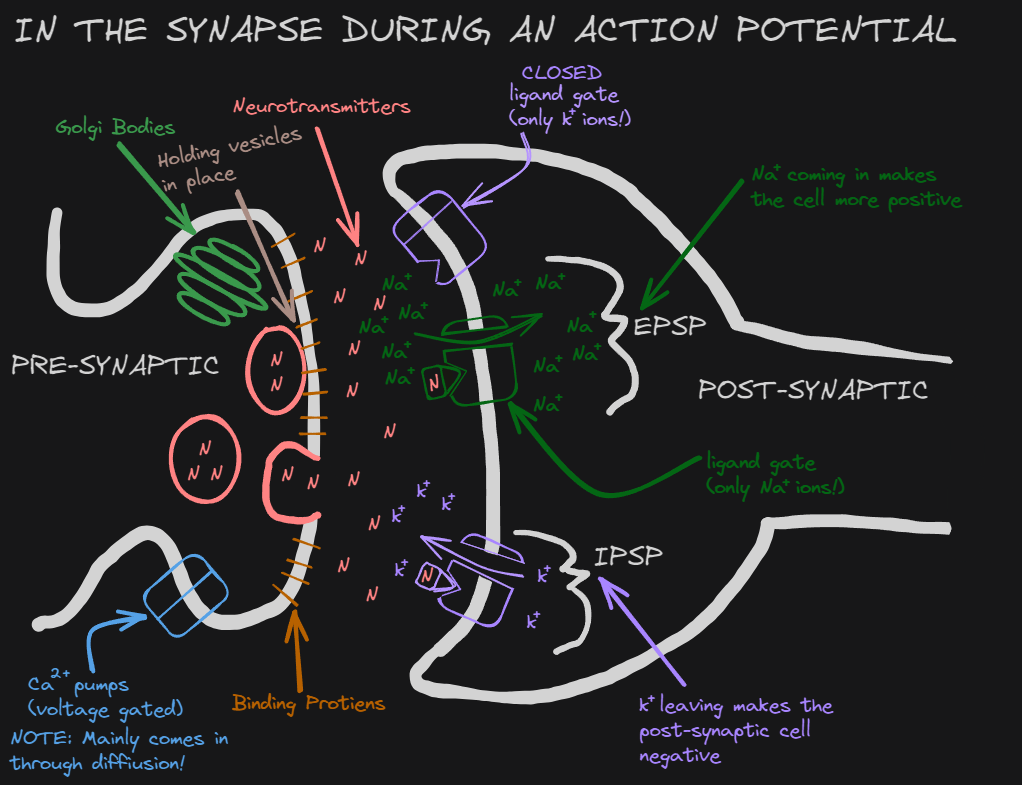
\includegraphics[width=.95\paperwidth,height=.95\paperheight,keepaspectratio]{excalidraw/neuron_synapse.png}
% \end{landscape}

% \begin{landscape}
%     \pagecolor{synapsebackground}
%     \pagestyle{plain}
%     \centering
%     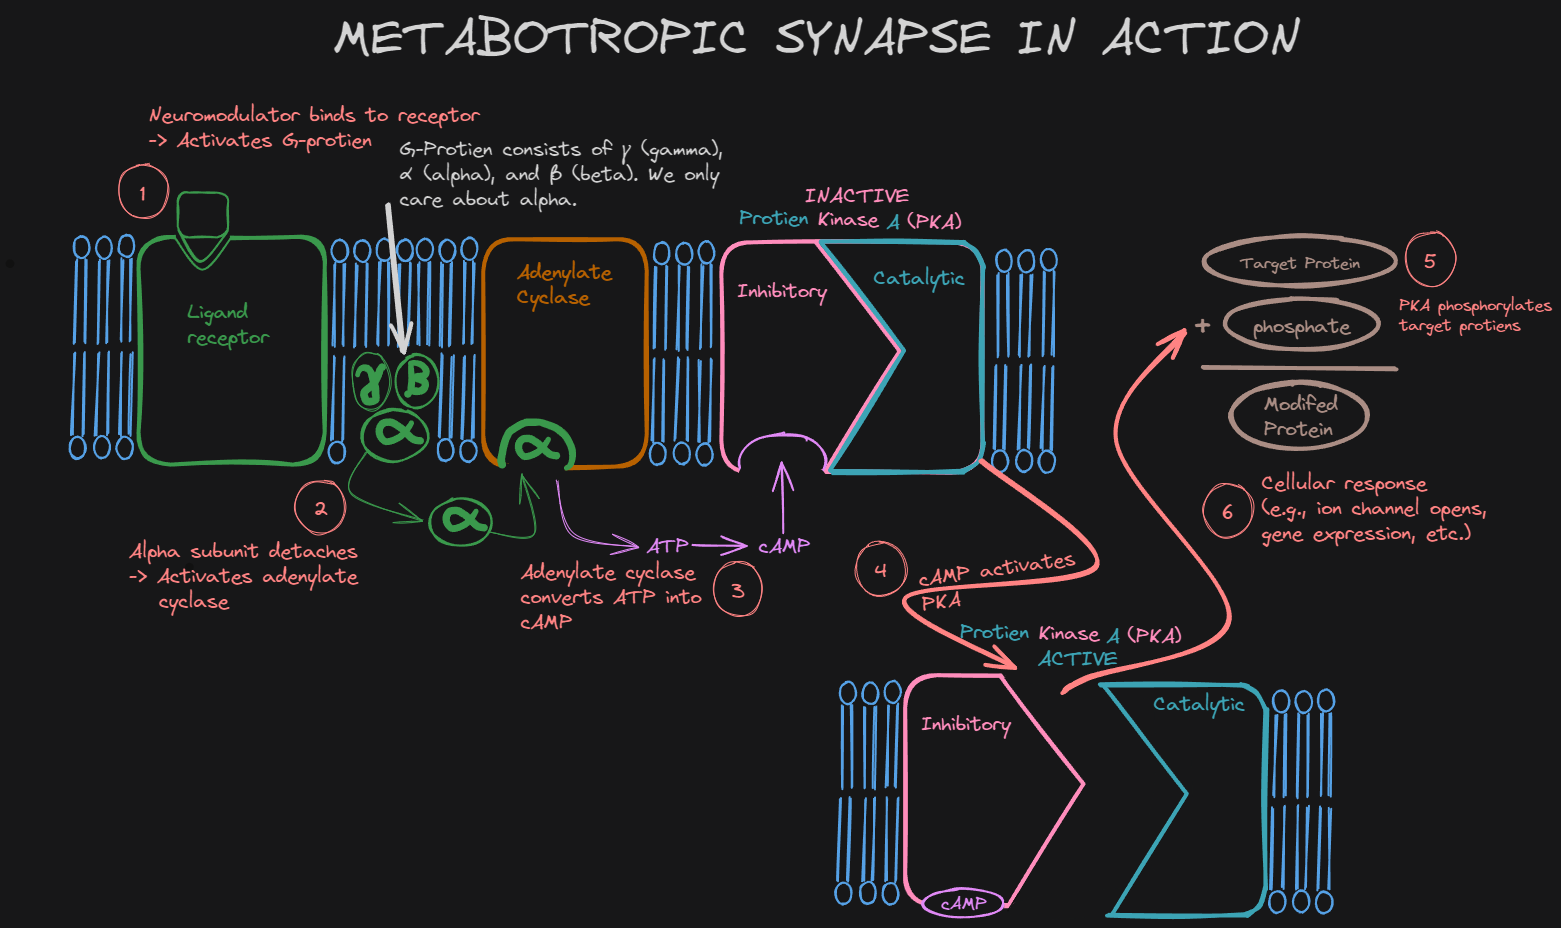
\includegraphics[width=.95\paperwidth,height=.95\paperheight,keepaspectratio]{excalidraw/metabotropic.png}
% \end{landscape}

% \pagecolor{draculabg}



\newpage
\begin{figure}[htbp]
    \centering
    \label{resting potential}
\begin{tikzpicture}
  % Labels for compartments
  \node at (-2,4.3) {\large \textbf{\underline{In}}};
  \node at (2,4.3) {\large \textbf{\underline{Out}}};
  \node at (-5.9,4.3) {\large \textbf{\underline{Permeability}}};

%   % Draw compartments as boxes
%   \draw (-5,-4) rectangle (-1,4); % Inside compartment
%   \draw (1,-4) rectangle (5,4);   % Outside compartment

  % Draw the membrane as a double line:
  % Left (solid) side denotes the negative (inside) and right (dotted) side the positive (outside)
  \draw[line width=1pt] (0.1,-4) -- (0.1,4);  
  \draw[dotted, line width=1pt] (-0.1,-4) -- (-0.1,4);

  % Place ion symbols on the "in" side (left) with relative sizes.
  % Here, potassium is large since it is more prevalent on the inside.
  \node (K_in) at (-3,2.5) {\huge \(\text{K}^{+}\)};
  \node (Na_in) at (-3,0) {\normalsize \(\text{Na}^{+}\)};
  \node (Cl_in) at (-3,-2.5) {\normalsize \(\text{Cl}^{-}\)};

  \node (P_K) at (-4.8,2.5) {\huge \(\text{P}\phantom{^{+}}\)};
  \node (P_K) at (-4.8,0) {\tiny \(\text{P}\phantom{^{+}}\)};
  \node (P_K) at (-4.8,-2.5) {\Large \(\text{P}\phantom{^{-}}\)};

  % Place ion symbols on the "out" side (right)
  % Here, sodium is made larger, etc.
  \node (K_out) at (3,2.5) {\normalsize \(\text{K}^{+}\)};
  \node (Na_out) at (3,0) {\huge \(\text{Na}^{+}\)};
  \node (Cl_out) at (3,-2.5) {\Large \(\text{Cl}^{-}\)};

  % Create nodes on the membrane for arrow connections
  \node (mem2_left) at (-0.5,0) {};
  \node (mem3_left) at (1.5,-2.5) {};
  \node (mem3_right) at (-1.5,-2.5) {};

  % Define arrow styles:
  \tikzset{
    diffusion/.style={->, >=Stealth, line width = 2pt, red},
    electric/.style={->, >=Stealth, line width = 2pt, blue}
  };

  % For each ion on the inside, draw two arrows (curved differently) going from the ion to the membrane.
  % The differences in the bending (and thus length) illustrate different magnitudes.
  % --- For K_in:
  \draw[electric, bend right=15] (K_in) to (K_out);
  \draw[diffusion, bend right=15, line width = 6pt] (K_out) to (K_in);
  % --- For Na_in:
  \draw[electric, bend left=15] (Na_out) to (mem2_left);
  \draw[diffusion, bend right=15] (Na_out) to (mem2_left);
  % --- For Cl_in:
  \draw[electric, bend right=15] (Cl_in) to (mem3_left);
  \draw[diffusion, bend right=15] (Cl_out) to (mem3_right);

  % Add a legend (key) to denote arrow styles.
  \node[draw, rectangle, right=1cm of K_out] (legend) {
    \begin{tabular}{ll}
      \textbf{Key:} & \\
      \tikz{\draw[diffusion, ->, >=Stealth, thick, red] (0,0) -- (1,0);} & Diffusion \\
      \tikz{\draw[electric, ->, >=Stealth, thick, blue] (0,0) -- (1,0);} & Electric \\
    \end{tabular}
  };
\end{tikzpicture}
\caption{The Resting Membrane Potential (RMP) of a Neuron}
\end{figure}

\begin{figure}[htbp]
    \centering
    \label{action potential}
\begin{tikzpicture}[scale=1.2]

    % Draw axes
    \draw[->, thick] (0,-4) -- (7,-4) node[right] {Time (ms)};
    \draw[->, thick] (0,-4) -- (0,3) node[above] {Voltage (mV)};

    % Draw threshold line at -55 mV and resting potential at -70 mV
    \draw[dashed] (0,-2.5) -- (7,-2.5) node[right] {Threshold (-55 mV)};
    \draw[dashed] (0,-3.5) -- (7,-3.5) node[right] {RMP (-70 mV)};
  
    % y-axis ticks and labels (scaling: 1 unit = 20 mV)
    \foreach \y/\label in {-3.5/{-70},-2.5/{-55}, -2/{-40}, -1/{-20}, 0/{0}, 1/{20}, 2/{40}} {
        \draw (0,\y) -- (-0.2,\y) node[left] {\label};
    }
    
    % x-axis ticks
    \foreach \x in {0,1,2,3,4,5,6} {
        \draw (\x,-4) -- (\x,-4.15) node[below] {\x};
    }
    
    % Draw action potential waveform using coordinates:
    % Points (x, y) where y = mV/20:
    % (0,-3.5):   Rest (-70 mV)
    % (1,-3.5):   Rest
    % (2,-2.75):  Threshold (-55 mV, since -55/20 = -2.75)
    % (3,2):      Peak depolarization (+40 mV, 40/20 = 2)
    % (4,-0.5):   Repolarization (-10 mV, -10/20 = -0.5)
    % (5,-4):     Hyperpolarization (-80 mV, -80/20 = -4)
    % (6,-3.5):   Return to rest (-70 mV)
    \draw[thick, horange] plot coordinates {
        (0,-3.5)
        (1,-3.5)
        (1.5,-3.5)
    };
    \draw[thick, horange, smooth] plot coordinates {
        (1.5,-3.5)
        (1.90,-2.55)
    };
    \draw[thick, horange] plot coordinates {
        (1.90,-2.55)
        (2,-2.5)
    };
    \draw[thick, horange, smooth] plot coordinates {
      (2,-2.5)
      (3,2)
      (4,-0.5)
      (5,-3.55)
      (6,-3.5)
    };

    % Add phase labels near the waveform
    \tikzset{
        circ/.style = {draw, circle, scale=0.7}
    };
    % Resting potential.
    \node[circ] at (1.3,-3.2) {1};
    % Opens sodium channels.
    \node[circ] at (1.75,-2.2) {2};
    % Potassium channels open.
    \node[circ] at (2.5,1.5) {3};
    % Sodium channels close.
    \node[circ] at (3.2,2.3) {4};
    % Potassium channels close.
    % \node[circ] at (6.1,-3.75) {5};
    
    \draw[decorate, decoration={brace, amplitude=5.5pt}]
    (5,-3.5) -- (6,-3.5);
    % Add text labels for phases
    \node at (2.2, 0) [rotate=78] {\textbf{Depolarization}};
    % The potassium is leaving the cell.
    \node at (4.2, 0) [rotate=287] {\textbf{Repolarization}};
    \node at (5.4, -3.1) {\textbf{Hyperpolarization}};

    % Arrow pointing hyperpolarization to -80 mv
    % \draw[->, thick] (7, -2) -- (4.93,-3.9) node[below] {};
  
  \end{tikzpicture}
    \caption{Action Potential Waveform}
\end{figure}



\setcounter{chapter}{6}
\chapter{Psychopharmacology}
\vspace*{-0.25in}
% \begin{center}
%     \textbf{NEW NOTES FOR 03/19/25} \\
%     \hrulefill
% \end{center}

\section{Overview -- Unit 3}

\begin{coloredlist}
    \item Neurotransmitters and Neuromodulators
    \begin{coloredlist}
        \item Psychopharmacology
        \item Disorders
        \item Pain
    \end{coloredlist}
\end{coloredlist}

\subsection{Psychopharmacology in Detail}

\begin{coloredlist}
    \item The scientific study of the effects of drugs on the nervous system and behavior.
    \item Psychopharmacology is the study of how drugs affect the mind and behavior.
    \begin{coloredlist}
        \item Psychotherapeutic drugs
        \item Better understanding of how things normally work.
    \end{coloredlist}
\end{coloredlist}

\subsubsection{Principles of Drug Action}

\begin{coloredlist}
    \item \cyanit{Selective Action} -- Drugs are selective in their action on the nervous system.
    \begin{coloredlist}
        \item \cyanit{Sites of Action} -- The location at which a drug interacts with the body to produce its effects.
        \item Side effects are often due to the drug acting on sites other than the intended target.
        \begin{coloredlist}
            \item Thus, side effects are relative to what our preferred site of action is.
        \end{coloredlist}
        \item \textit{Example}: Opioids primarily affect the opioid receptor system.
    \end{coloredlist}
    \item Drugs don't CREATE effects, they \textit{modulate} ongoing cellular activity.
    \begin{coloredlist}
        \item That is, they affect behavior by affecting neural transmission in some way.
        \item \cyanit{Agonist} -- A drug that mimics or enhances the \textbf{effects of a neurotransmitter}.
        \begin{coloredlist}
            \item Facilitates post synaptic effects.
            \item \textit{Example}: Morphine mimics endorphins, which are natural painkillers.
        \end{coloredlist}
        \item \cyanit{Antagonist} -- A drug that blocks or inhibits the effects of a neurotransmitter.
        \begin{coloredlist}
            \item Inhibits post synaptic effects.
            \item \textit{Example}: Naloxone blocks the effects of opioids, reversing their effects.
        \end{coloredlist}
        \item Agonistic effects can become antagonistic if the drug is taken in excess.
        \begin{coloredlist}
            \item \textit{Example}: I make a neuron fire a neurotransmitter, but I also block the reuptake of that neurotransmitter.
        \end{coloredlist}
    \end{coloredlist}
\end{coloredlist}

\subsubsection{Basic Process}

\begin{coloredlist}
    \item \cyanit{Precursor} -- A substance from which another substance is formed. AKA, the ingredients used to make a neurotransmitter.
    \item \[
        \text{Precursor} \xrightarrow{\text{Synthetic Enzyme}} \text{NT} \xrightarrow{\text{Metabolic Enzyme}} \text{Inactive Metabolite}
    \]
    \begin{coloredlist}
        \item \cyanit{Synthesis} -- The process of creating a neurotransmitter from its precursors.
        \item Sometimes, we break down the precursor to build the neurotransmitter.
        % \item \cyanit{Storage} -- The neurotransmitter is stored in vesicles until it is needed.
        % \item \cyanit{Release} -- The neurotransmitter is released into the synaptic cleft when an action potential arrives at the axon terminal.
        % \item \cyanit{Binding} -- The neurotransmitter binds to receptors on the post-synaptic neuron, causing a change in the neuron's activity.
        % \item \cyanit{Inactivation} -- The neurotransmitter is removed from the synaptic cleft by reuptake or enzymatic degradation.
    \end{coloredlist}
\end{coloredlist}

% \begin{center}
%     \textbf{NEW NOTES FOR 03/21/25} \\
%     \hrulefill
% \end{center}

\subsection{Other Ways of Agonist and Antagonist}

\begin{coloredlist}
    \item Block Ca\(^{2+}\) channels from opening (antagonist)
    \item \cyanit{Mimetic} -- Mimics the action of a neurotransmitter.
    \begin{coloredlist}
        \item \cyanit{Direct Agonist} -- Binds to the same receptor as the neurotransmitter and mimics its effects.
        \item \cyanit{Indirect Agonist} -- Binds to a different site on the receptor and enhances the effects of the neurotransmitter.
    \end{coloredlist}
    \item Blocking agent
    \begin{coloredlist}
        \item Competitive
        \begin{coloredlist}
            \item \cyanit{Direct Antagonist} -- Binds to the same receptor as the neurotransmitter and blocks its effects.
        \end{coloredlist}
        \item Non-competitive
        \begin{coloredlist}
            \item \cyanit{Indirect Antagonist} -- Binds to a different site on the receptor and blocks the effects of the neurotransmitter.
        \end{coloredlist}
        \item \cyanit{Inverse Agonist} -- Binds to the same receptor as the neurotransmitter and produces the opposite effect.
    \end{coloredlist}
    \item \cyanit{Depolarizing} or \cyanit{Desensitizing Agent} -- A drug that causes the AP to stay in a depolarized state; refusing to let the neuron go through another AP, and it stays in the absolute refractory period. (Antagonist)
    \item Interfere with vesicles (leaky or transporter proteins). (Antagonist)
    \item Interfere with docking proteins. (Antagonist)
    \item Selectively deactivate autoreceptors. (Agonist)
    \item Selectively activate autoreceptors. (Antagonist)
\end{coloredlist}

\section{What Do These Chemicals Between Neurons Do?}

\begin{coloredlist}
    \item Transmit information.
    \begin{coloredlist}
        \item Glutamate
        \item GABA
        \item Glycine
    \end{coloredlist}
    \item Modulate information.
    \begin{coloredlist}
        \item Every other neurotransmitter.
    \end{coloredlist}
\end{coloredlist}

\section{Classes of Neurotransmitters (Revisited from Lab)}

\begin{coloredlist}
    \item Amino Acids
    \begin{coloredlist}
        \item Glutamate, GABA, Glycine
        \begin{coloredlist}
            \item \cyanit{Glutamate} -- Synthesized from precursor glutamine by an enzyme called \cyanit{glutaminase}. It is the most common excitatory neurotransmitter in the brain.
            \begin{coloredlist}
                \item Related closely with the \cyanit{NMDA} receptor, which is a type of glutamate receptor that is important for synaptic plasticity and memory formation.
                \item One drug that binds to this site, \cyanit{Phencyclidine (PCP)} (direct antagonist), is a drug that blocks the NMDA receptor and causes hallucinations and dissociation. Another drug that is thought to bind here, \cyanit{Ketamine} (direct antagonist), is a dissociative anesthetic that is used in surgery and is also being studied as a treatment for depression.
                \item \textbf{Reuptake and Deactivation}
                \begin{coloredlist}
                    \item Reuptake is done by the \cyanit{excitatory amino acid transporters (EAATs)}. These are important because it reduces the change of excitotoxicity, which is believed to be involved in damage to the brain in stroke and amyotrophic later sclerosis (ALS, Lou Gehrig's disease).
                \end{coloredlist}
            \end{coloredlist}
            \item \cyanit{GABA} -- Synthesized from precursor glutamate by an enzyme called \cyanit{glutamic acid decarboxylase (GAD)}. It is the most common inhibitory neurotransmitter in the brain.
        \end{coloredlist}
    \end{coloredlist}
    \item \cyanit{Amines} (monoamines) -- Derived from amino acids
    \begin{coloredlist}
        \item Catecholamines
        \begin{coloredlist}
            \item Contain catechol and derived from the amino acid tyrosine.
            \item \cyanit{Tyrosine} -- Precursor for the catecholamines.
            \item Dopamine (DA), Norepinephrine (NE), Epinephrine (Adrenaline)
            \item Dopaminergic, Adrenergic, and Noradrenergic systems.
        \end{coloredlist}

        % \begin{center}
        %     \textbf{New Notes for 03/31/25} \\
        %     \hrulefill
        % \end{center}

        \item \cyanit{Indolamines} %-- Derived from the amino acid tryptophan.
        \begin{coloredlist}
            \item \cyanit{Serotonin} (5-HT) %-- Derived from the amino acid tryptophan.
            \item \cyanit{Melatonin} %-- Derived from serotonin.
        \end{coloredlist}
        \item Peptides (AKA: Neuropeptides)
        \begin{coloredlist}
            \item Endogenous Opioids
        \end{coloredlist}
        \item Acetylcholine (ACh)
        \item Lipids
        \begin{coloredlist}
            \item \cyanit{Anadamide} (Sanskrit for ``bliss'') -- Endogenous cannabinoid.
            \item These appear to be synthesized on demand; produced and released as needed and not stored in synaptic vesicles.
            \item Anadamide is deactivated by the enzyme \cyanit{fatty acid amide hydrolase (FAAH)}.
        \end{coloredlist}
        \item \textbf{Two Other Classes}
        \begin{coloredlist}
            \item Nucleosides
            \begin{coloredlist}
                \item Adenosine
            \end{coloredlist}
            \item Soluble Gases
            \begin{coloredlist}
                \item \cyanit{Nitric Oxide (NO)} -- Required for an erection.
            \end{coloredlist}
        \end{coloredlist}
    \end{coloredlist}
\end{coloredlist}

\section{Acetylcholine (ACh)}

\begin{coloredlist}
    \item First neurotransmitter discovered.
    \begin{coloredlist}
        \item Otto von Loewy -- Discovered ACh in 1921.
        \begin{coloredlist}
            \item This guy took a frog heart and put it in saline. Then, he took simulated the parasympathetic part of the vagus nerve, and saw that the heart slowed down.
            \item He then took the saline and put it in a different frog heart, and saw that the heart slowed down again.
            \item ``Vagusstoff'' (ACh) -- The chemical that was released from the vagus nerve that slowed the heart down.
            \item Cholinergic -- Referring to ACh.
        \end{coloredlist}
    \end{coloredlist}
    \item \textbf{\textit{Some} Functions}
    \begin{coloredlist}
        \item \textbf{Function in the ANS:}
        \begin{coloredlist}
            \item Sympathetic
            \begin{coloredlist}
                \item Spinal nerve leaves the cord and synapses in the paravertebral ganglion (ACh)
                \item Then makes neuromuscular junction with smooth muscles and glands (NE)
                \begin{coloredlist}
                    \item \cyanit{Neuromusclar Junction} -- The synapse between a motor neuron and a muscle fiber.
                    \item \cyanit{Paravertebral Ganglion} -- A ganglion located next to the spinal cord.
                \end{coloredlist}
                \begin{coloredlist}
                    \item Except sweat glands (ACh)
                \end{coloredlist}
                \item \cyanit{Sympathetic Chain} -- A chain of ganglia that runs parallel to the spinal cord. This is the reason for when you get anxious, ALL of your body gets anxious.
            \end{coloredlist}
            \item Parasympathetic
            \begin{coloredlist}
                \item Spinal nerve leaves the cord and synapse in the parasympathetic ganglion (ACh)
                \item Then makes neuromuscular junction with smooth muscles and glands (ACh)
            \end{coloredlist}
            \item The only NT in the parasympathetic branch.
            \item NT of the preganglionic sympathetic branch.
        \end{coloredlist}
        \item \textbf{Function in the Somatic NS}
        \begin{coloredlist}
            \item Excites the neuromusclar junction (ACh)
            \item So, ACh is important for getting motor messages out to all kinds of muscles and glands.
        \end{coloredlist}
        % \begin{center}
        %     \textbf{NEW NOTES FOR 04/02/25} \\
        %     \hrulefill
        % \end{center}
        \item \textbf{Function in the CNS}
        \begin{coloredlist}
            \item ACh is important in:
            \begin{coloredlist}
                \item Learning and alertness (\cyanit{Basal Forebrain})---activates the cortex and facilitates learning.
                \begin{coloredlist}
                    \item \cyanit{Nucleus Basalis} -- Projects to the cortex
                    \item \cyanit{Medial Septal Nucleus} and \cyanit{Nucleus of Diagonal Band} -- Projects to the hippocampus through the fornix.
                \end{coloredlist}
                \item Memory (\cyanit{medial septal nucleus})---modulate the hippocampus
                \item REM sleep generation (\cyanit{Pedunculopontine nucleus (PPT)} and \cyanit{Laterodorsal Tegmental Nucleus (LDT)})---projects to the pons and thalamus.
                \item Reward system.
            \end{coloredlist}
        \end{coloredlist}
    \end{coloredlist}
    \item \textbf{Synthesis and Metabolism}
    \item \textbf{Drugs and Disorders}
\end{coloredlist}

\subsection{ACh Synthesis and Metabolism}

\begin{coloredlist}
    \item \textbf{Synthesis}
    \begin{coloredlist}
        \item In a nutshell: A breakdown of lipids leads to Choline, which is the precursor for ACh. Acetate is the anion in vinegar (Acetic acid). Then, this is combined with Acetate to make ACh.
        \item In more detail:
        \begin{coloredlist}
            \item CoA attaches to an acetate ion (\cyanit{Acetylcoenzyme A (acetyl-CoA)}).
            \item Then, \cyanit{choline acetyltransferase (ChAT)} transfers the acetate from the acetyl-CoA to the choline molecule.
            \item Mnemonic: \textbf{ChAT}: From right to left: Transfers acetate to choline.
        \end{coloredlist}
    \end{coloredlist}
    \item \textbf{Metabolism}
    \begin{coloredlist}
        \item ACh is broken down by the enzyme \cyanit{acetylcholinesterase (AChE)} into acetate and choline. Nice and simple!
        \item The choline is taken back up by active transport and reused, and the acetate is broken down and eliminated.
    \end{coloredlist}
\end{coloredlist}

\subsection{Two Types of Cholinergic Receptors}

\begin{coloredlist}
    \item Nicotinic Receptors
    \begin{coloredlist}
        \item Agonist at low doses, but antagonist at high doses.
        \item Iontropic.
        \item Found at the Neuromusclar Function in the PNS.
        \item \cyanit{Curare} (direct antagonist) -- A drug that blocks nicotinic receptors, causing paralysis.
        \begin{coloredlist}
            \item Competitive blocking agent
            \item Paralysis, surgery
        \end{coloredlist}
    \end{coloredlist}
    \item Muscarinic Receptors
    \begin{coloredlist}
        \item Comes from a hallucinogenic mushroom (Amanita muscaria).
        \begin{coloredlist}
            \item \textbf{Don't confuse with Serotonin's Mescaline: Cactus; nor Psilocybin: Mushroom.}
        \end{coloredlist}
        \item Vikings (probably took this drug before raiding) and Koryaks (Nordic people who used this mushroom in religious practices).
        \item Metabotropic receptors.
        \item Predominates in the CNS (although, both types are found in the CNS).
        \item \cyanit{Atropine} (direct antagonist) -- A drug that blocks muscarinic receptors, causing pupil dilation and increased heart rate.
        \begin{coloredlist}
            \item Competitive blocking agent
            \item Belladonna alkaloids (deadly nightshade)
        \end{coloredlist}
    \end{coloredlist}
\end{coloredlist}

% \begin{center}
%     \textbf{NEW NOTES FOR 04/04/25} \\
%     \hrulefill
% \end{center}

\section{MORE Drugs and Toxins Affecting ACh}

\begin{coloredlist}
    \item \cyanit{Botulinum Toxin} -- A waste product of \textit{Clostridium botulinum}, which are bacteria who grows without oxygen.
    \begin{coloredlist}
        \item Interferes with Ca\(^{2+}\) influx channels, preventing the release of ACh.
        \item Because Botox causes paralysis, it can interfere with emotional \textit{expression} because it paralyzes muscles like the orbicularis oculi.
        \item Additionally, since we know that expression influences experience, when we paralyze these muscles, then the emotional \textit{experience} is also negatively affected.
        \item \textbf{Does Botox Decrease Emotional Experiences?}
        \begin{coloredlist}
            \item Population: Women who want wrinkles gone.
            \item One IV: two levels: Botox or restylane (dermal filler).
            \item Method: Everyone had wrinkle reduction. AND, Everyone watches some emotion evoking movies.
            \item Results: Botox group had less emotional experience than the restylane group.
            \item \textbf{Is this a good thing?}
            \begin{coloredlist}
                \item Another study takes a sample of depressed people and gives them either Botox or a placebo.
                \item Results: 15\% of placebo had a decrease in depression, while 52\% of the Botox group had a decrease in depression.
            \end{coloredlist}
        \end{coloredlist}
        \item Botox can also be used to treat migraines, cerebral palsy, and hyperhidrosis (excessive sweating).
    \end{coloredlist}
    \item \cyanit{Black Widow Spider Venom} -- A neurotoxin that causes the release of ACh at the neuromuscular junction, causing continual release of ACh and paralysis.
    \item \cyanit{Cobra and Krait Venom} -- A neurotoxin that blocks the binding of ACh to nicotinic receptors, causing paralysis.
    \item \cyanit{AchE Blockers} -- Comes into contact with the enzyme that breaks down ACh, causing an increase in ACh in the synaptic cleft.
    \begin{coloredlist}
        \item Irreversible
        % \begin{center}
        %     \textbf{NEW NOTES FOR 04/07/25} \\
        %     \hrulefill
        % \end{center}
        \begin{coloredlist}
            \item Insecticides (Parathion)
            \item Nerve gas: DFP (Diisopropylfluorophosphate (don't need to know the whole name)) and Sarin.
            \begin{coloredlist}
                \item Readily crosses the blood-brain barrier so PNS and CNS are affected.
                \item Antidote?
                \begin{coloredlist}
                    \item \cyanit{Atropine} -- A drug that blocks muscarinic receptors, preventing the effects of excess ACh.
                    \item \cyanit{Pralidoxime} -- A drug that reactivates AChE, allowing it to break down ACh again.
                \end{coloredlist}
            \end{coloredlist}
        \end{coloredlist}
        \item Reversible
        \begin{coloredlist}
            \item \cyanit{Neostgmine} (\textbf{Prostigmin}) and \cyanit{Physostigmine} (\textbf{Antilirum}) -- Drugs that inhibit AChE, increasing the amount of ACh in the synaptic cleft.
            \begin{coloredlist}
                \item Doesn't cross the blood-brain barrier, so it only affects the PNS.
                \item Used to treat \cyanit{myasthenia gravis} (a disease that causes muscle weakness and fatigue).
                \begin{coloredlist}
                    \item Autoimmune disease that attacks nicotinic receptors at the neuromuscular junction.
                \end{coloredlist}
            \end{coloredlist}
            \item \cyanit{Donepezil} (\textbf{Aricept}) and \cyanit{rivastigmine} (\textbf{Exelon}) -- These drugs do the same thing as the above drugs, but they cross the blood-brain barrier and are used to treat Alzheimer's disease and Parkinson's disease (only the cognitive part).
        \end{coloredlist}
    \end{coloredlist}
\end{coloredlist}

\section{New Drug for Schizophrenia}

\begin{coloredlist}
    \item We'll talk about dopamine drugs later in this unit.
    \item This new drug now:
    \begin{coloredlist}
        \item \cyanit{Xanomelne and trospium chloride} (\textbf{Cobenfy}) -- A drug that blocks the muscarinic receptors in the CNS, but not in the PNS.
        \item Dopamine but also Ach!
    \end{coloredlist}
\end{coloredlist}

\section{Catecholamines}

\begin{coloredlist}
    \item Dopamine (DA)
    \item Norepinephrine (NE)
    \item Epinephrine (Adrenaline)
\end{coloredlist}

\subsection{Dopamine (DA)}

\begin{coloredlist}
    \item Synthesis and Metabolism
    \item Function
    \item Drugs and Disorders
\end{coloredlist}

\subsubsection{Dopamine Synthesis}

\begin{coloredlist}
    \item Tyrosine was first discovered from cheese (tyrosine = cheese).
    \begin{coloredlist}
        \item Tyrosine is the precursor for DA, NE, and Epi.
        \item \cyanit{Tyrosine Hydroxylase} -- The rate-limiting enzyme in the synthesis of catecholamines.
        \begin{coloredlist}
            \item Converts tyrosine to L-DOPA.
            \item L-DOPA is the precursor for DA, NE, and Epi.
        \end{coloredlist}
        \item L-DOPA is converted to DA by the enzyme \cyanit{DOPA decarboxylase}.
        % \item DA is converted to NE by the enzyme \cyanit{Dopamine \(\beta\)-hydroxylase (DBH)}.
        % \item NE is converted to Epi by the enzyme \cyanit{Phenylethanolamine N-methyltransferase (PNMT)}.
    \end{coloredlist}
\end{coloredlist}

\subsubsection{Dopamine Metabolism}

\begin{coloredlist}
    \item DA is broken down by the enzyme \cyanit{Monoamine Oxidase (MAO)} into \cyanit{Dihydroxyphenylacetric acid (DOPAC)}.
    \item Then, \cyanit{Catechol-O-methyltransferase (COMT)} converts DOPAC into \cyanit{Homovanillic acid (HVA)}.
    \item Also, starting from DA, we can use COMT to convert it to 3-methoxytyramine (3-MT), then with MAO, we can convert it to HVA.
\end{coloredlist}

\subsubsection{DA Function}

\begin{coloredlist}
    \item \textbf{Movement/Motor systems}
    \begin{coloredlist}
        \item \cyanit{Nigrostriatal System} -- Starts in the substantia nigra and ends in the striatum (caudate nucleus and putamen).
        \item Here's the route: We start at the striatum, which then sends an inhibitory GABA signal to the substantia nigra, who sends a reciprocal inhibitory DOPA signal back to the striatum nerve that sends an inhibitory GABA signal to the globus pallidus. Then, the globus pallidus excites the thalamus, who then excites the primary motor cortex, who then excites movement.
        \begin{coloredlist}
            \item Note that if the inhibitory signal to the substantia nigra is limited, then the signal that the striatum sends to the globus pallidus is much stronger, which leads to a weaker signal to the thalamus, and thus to movements.
        \end{coloredlist}
        \item Parkinson's Disease symptoms:
        \begin{coloredlist}
            \item Weakness,
            \item Tremor at rest,
            \item Muscle rigidity,
            \item Problems with balance,
            \item Abnormal gait,
            \item Trouble learning
        \end{coloredlist}
        \item Treatment
        % \begin{center}
        %     \textbf{NEW NOTES FOR 04/09/25} \\
        %     \hrulefill
        % \end{center}
        \begin{coloredlist}
            \item \cyanit{Reserpine} (\textbf{Raudixin}) for \(\downarrow\) \textbf{BP} (Not in use anymore because it caused Parkinson's-like symptoms)
            \begin{coloredlist}
                \item 1960's
                \begin{coloredlist}
                    \item Blocks monoamine transporters
                    \begin{coloredlist}
                        \item Developed Parkinson's symptoms
                        \item Can't fill vesicles and DA is lowered
                    \end{coloredlist}
                \end{coloredlist}
                \item Then, discovered Substantia Nigra was pale.
            \end{coloredlist}
            \item L-DOPA can be a direct treatment for Parkinson's as well.
            \item \cyanit{MPTP} -- Neurotoxin for DA cells in the Nigrostriatal System (which is not endogenous).
            \item \textbf{History of MPTP -- or why you shouldn't use illicit drugs}
            \begin{coloredlist}
                \item 1982 -- young California heroin users
                \item Had used what they THOUGHT was synthetic heroin
                \begin{coloredlist}
                    \item \cyanit{MPPP} -- Opioid analgesic drug
                    \begin{coloredlist}
                        \item Not used clinically
                        \item Illegally manufactured for recreational drug use
                    \end{coloredlist}
                    \item INSTEAD it was MPTP (oh no!)
                    \begin{coloredlist}
                        \item They instantly developed Parkinson's-like symptoms
                        \item Bad for them, but good for us because we can study it.
                        \begin{coloredlist}
                            \item Led to animal model development and possible treatment ideas.
                        \end{coloredlist}
                    \end{coloredlist}
                \end{coloredlist}
                \item We don't know why Parkinson's patient's cells are dying, but maybe something similar.
                \item MPTP is converted to the chemical \cyanit{MPP+} by the enzyme MAO (which is what breaks down DA), which is what damaged the cells.
                \begin{coloredlist}
                    \item Question: Could MAO-I improve Parkinson's?
                    \item Yes!
                    \item \cyanit{Deprenyl}, also called \cyanit{selegiline} (\textbf{Eldepryl}, \textbf{Jumex}) -- A drug that inhibits MAO, can slow down progression of the disease.
                \end{coloredlist}
            \end{coloredlist}        
        \end{coloredlist}
        \item New treatment
        \begin{coloredlist}
            \item Molecule keeps proteins from misfolding
            \item \cyanit{Lewy Bodies} -- Misfolded proteins that are found in the brains of people with Parkinson's.
            \begin{coloredlist}
                \item These are toxic to DA cells
            \end{coloredlist}
        \end{coloredlist}
        \item \cyanit{Huntington's Chorea} -- A genetic disorder that leads to uncontrolled movements and cognitive decline.
        \begin{coloredlist}
            \item Too little GABA from the Striatum to the Substantia Nigra causes an increase in dopamine back to the Striatum which, in turn, lessens the signal to the Globus Palidus, which increases overall movements.
            \item \cyanit{Tetrabenazine} (\textbf{Xenazine}) -- Drug that inhibits the DA vesicle transporters.
            \item \cyanit{Pallidotomy} -- A surgery that affects the Globus Pallidus to inhibit movement.
        \end{coloredlist}
        \item \cyanit{Choreoathetotic Movements} -- too much movement
        \begin{coloredlist}
            \item \cyanit{Athetosis} -- Slow continually writing movements
            \item \cyanit{Choreic} (to dance) -- Rapid, purposeless, involvuntary movements
        \end{coloredlist}
        % \begin{center}
        %     \textbf{NEW NOTES FOR 04/11/25} \\
        %     \hrulefill
        % \end{center}
    \end{coloredlist}
    \item \textbf{Behavioral Arousal and Attention}
    \begin{coloredlist}
        \item Narcolepsy
        \begin{coloredlist}
            \item \cyanit{Methylphenidate} (\textbf{Ritalin}) -- A drug that increases DA and NE in the brain, used to treat ADHD, but can also be used for narcolepsy.
            \item \cyanit{Hypocretine} -- A neuropeptide that is involved in the regulation of sleep and wakefulness.
            \begin{coloredlist}
                \item Created by the lateral hypothalamus.
                \item Hypocretine: \textit{Hypo} for \textit{hypo}thalamus, \textit{cretine} for \textit{secretin} (a hormone).
                \item \cyanit{Orexin} -- Another name for hypocretine; makes you want to eat.
            \end{coloredlist}
            \item From hypocretine, researchers developed an antagonist for the orexin receptor, which is used to treat insomnia. This drug is called \cyanit{Suvorexant} (\textbf{Belsomra}).
            \item \textbf{Treatment}
            \begin{coloredlist}
                \item \cyanit{TAK-994} -- OX2R (Orexin-2 receptor) Agonist
                \item \cyanit{Hcrt-1} -- Intranasal hypocretine-1 (orexin-1) agonist
                \item Hypocretine Cell Transplant
                \item Gene Therapy: \textit{introduce} preprohypocretin gene into the brain to make more hypocretine.
                \item Opiates (exogenous) can increase the number of hypocretin-producing cells in the brain.
                \item Indirect role for opiate agonists in treating narcolepsy.
            \end{coloredlist}            
        \end{coloredlist}
        \item ADHD
        \begin{coloredlist}
            \item Uses Methylphenidate for selective attention.
        \end{coloredlist}
        \item \cyanit{Mesocortical System}
        \begin{coloredlist}
            \item From ventral tegmental nucleus to prefrontal cortex, limbic CORTEX, hippocampus, all frontal lobes, and association areas of parietal and temporal lobes in primates.
            \item Short-term memories, planning, and problem-solving are all associated with this system.
        \end{coloredlist}
    \end{coloredlist}
    \item \textbf{Reinforcement and Reward}
    \begin{coloredlist}
        \item \cyanit{Mesolimbic System (MLS)} -- Responsible for reward and reinforcement.
        \begin{coloredlist}
            \item From vental tegmental nucleus to limbic system
            \begin{coloredlist}
                \item Amygdala, hippocampus, and nucleus accumbens.
                \item Opioids cause the release of dopamine at the nucleus accumbens, which is the pleasure center of the brain.
            \end{coloredlist}
        \end{coloredlist}
        \item James Olds \& Peter Milner (1954)
        \begin{coloredlist}
            \item They asked: ``Does electrical stimulation of the reticular formation facilitate learning?''
            \item James Olds visits a conference and listens to Neal Miller, who says electrical stimulation is aversive, so it should be avoided.
            \item One lone rat was put in a box with a lever, and when the rat pressed the lever, it would get a shock to the reticular formation. He ended up pressing the level 700 times per hour.
        \end{coloredlist}
        \item More studies of this
        \begin{coloredlist}
            \item Skinner box
            \begin{coloredlist}
                \item Rats press 2000 times per hour for a shock to the MLS.
                \item Monkeys press 8000 times per hour for a shock to the MLS.
                \item Starving animals will choose the MLS over food 80\% of the time. 
                \item They also press the button for these conditions too:
                \begin{coloredlist}
                    \item Thirsty,
                    \item Getting shocked (at their feet),
                    \item Mother instincts.
                \end{coloredlist}
            \end{coloredlist}
        \end{coloredlist}
        \item Delgado (1969) -- For people who were getting their brain stimulated for seizures, this researcher also asked them about what they thought of the stimulation. They all thought that it was pleasurable.   
    \end{coloredlist}
\end{coloredlist}

\begin{center}
    \textbf{NEW NOTES FOR 04/16/25} \\
    \hrulefill
\end{center}

\section{Schizophrenia in Focus}

\subsection{General Description}

\begin{coloredlist}
    \item \cyanit{Dementia Praecox} -- A term used to describe a group of disorders characterized by a decline in cognitive function and emotional regulation. Found by Emil Kraepelin, a German psychiatrist (1887).
    \begin{coloredlist}
        \item Premature deterioration of the mind.
    \end{coloredlist}
    \item Age of onset: Late teens to mid 30s.
    \item \cyanit{Schizophrenia} -- Same definition as before, duh. Found by Eugen Bleuler, a Swiss psychiatrist (1911).
    \begin{coloredlist}
        \item Split of the mind from reality, not split personalities.
    \end{coloredlist}
\end{coloredlist}

\subsection{Theory behind Negative and Positive Symptoms**}
**(and Cognitive Symptoms)
\begin{coloredlist}
    \item ``Positive'' and ``Negative'' are not used in the traditional sense. Instead, they are used to describe the presence or absence of certain symptoms.
    \begin{coloredlist}
        \item Positive symptoms are the presence of abnormal behaviors, while negative symptoms are the diminution or absence of normal behaviors.
        \item Cognitive symptoms are the presence of cognitive deficits.
    \end{coloredlist}
\end{coloredlist}

\subsubsection{Positive Symptoms (Escalation over normal functioning)}

\begin{coloredlist}
    \item \cyanit{Hallucinations} -- Perception of something that does not have a basis in reality.
    \begin{coloredlist}
        \item Auditory (most common), visual, tactile, olfactory, and gustatory.
    \end{coloredlist}
    \item \cyanit{Delusions} -- A false belief that is resistant to reason or confrontation with actual fact. Actually built on reality, but misinterpreted.
    \begin{coloredlist}
        \item Patently unrealistic.
        \item For example:
        \begin{coloredlist}
            \item \cyanit{Referential} -- Believing that something is meant for you (e.g., the TV is talking to you).
            \item \cyanit{Persecutory} -- Believing that someone is out to get you (e.g., the government is watching you).
            \item \cyanit{Grandiose} -- Believing that you are more important than you are (e.g., you are the king of the world).
            \item \cyanit{Control} -- Believing that someone is controlling your thoughts or actions (e.g., the government is controlling your mind).
        \end{coloredlist}
        \item On the difference between an \textit{illusion} and a \textit{delusion} is that everyone can experience and illusion (not unique and based on manipulations of our nervous systems), whereas a delusion is unique to the person experiencing.
    \end{coloredlist}
    \item \cyanit{Disorganized Speech} -- A pattern of incoherent or illogical speech that is difficult to follow.
    \begin{coloredlist}
        \item \cyanit{Derailment} -- A pattern of speech in which the speaker jumps from one topic to another without any logical connection between them.
        \item \cyanit{Tangentiality} -- A pattern of speech in which the speaker goes off on tangents and does not return to the main topic.
        \item \cyanit{Word Salad} -- A pattern of speech in which the speaker uses words that are not related to each other in any meaningful way.
    \end{coloredlist}
    \item \cyanit{Grossly disorganized behavior} -- A pattern of behavior that is inappropriate for the situation or that is not goal-directed. It is unpredictable and unprovoked.
    \item \cyanit{Catatonic behavior} -- A pattern of behavior in which the person is unresponsive to the environment and does not move or speak.
    \begin{coloredlist}
        \item Maintaining a rigid or bizarre posture.
        \item Purposeless excessive motor activity.
        \begin{coloredlist}
            \item For example, continuously spinning your hair in circles or pacing back and forth.
        \end{coloredlist}
    \end{coloredlist}
\end{coloredlist}

\subsubsection{Negative Symptoms}

\begin{coloredlist}
    \item \cyanit{Affective Flattening} -- Restricted range of emotional expression, including facial expressions, voice tone, and body language.
    \item \cyanit{Alogia} -- A lack of speech or a decrease in the amount of thought, which is reflected in a decrease in speech produced.
    \item \cyanit{Avolition} -- A lack of motivation or a decrease in the ability to initiate and persist in activities.
    \item \cyanit{Anhedonia} -- A lack of pleasure or a decrease in the ability to experience pleasure from activities that are normally pleasurable.
    \item Notice that these negative symptoms are shared with a lot of other disorders, including depression and anxiety, or even brain damage.
\end{coloredlist}

\subsubsection{Positive versus Negative (Summary)}

\begin{coloredlist}
    \item Positive
    \begin{coloredlist}
        \item Relatively unique and historically easier to treat.
    \end{coloredlist}
    \item Negative
    \begin{coloredlist}
        \item Common in a number of disorders.
        \item Less responsible to treatment.
        \item Usually emerge first.
    \end{coloredlist}
\end{coloredlist}

\begin{center}
    \textbf{NEW NOTES FOR 04/18/25} \\
    \hrulefill
\end{center}

\subsection{Negative Symptoms and Brain Damage}

\begin{coloredlist}
    \item \cyanit{Discordant Twins} -- Twins that are discordant for a disorder, meaning that one twin has the disorder and the other does not. 
    \item Brain atrophy is larger than normal ventricles and cortical sulci.
    \item Abnormal neurological systems (physiological tests that are used to assess the function of the nervous system).
    \begin{coloredlist}
        \item Jerky or non-existent visual pursuit, and cannot do it without moving their head.
        \item Absence of a blink reflex.
        \item Poor pupillary light reactions.
        \item Unusual facial expressions.
        \item Continuous elevation of the eyebrows.
    \end{coloredlist}
    \item \cyanit{Cytoarchitectual Abnormalities} -- Abnormalities in the structure of the brain cells and their organization.
    \begin{coloredlist}
        \item \textbf{Hippocampus} -- Cell bodies are aligned with healthy people, but not aligned for people with schizophrenia. It indicates that this is a developmental disorder.
        \item List of reasons for why these abnormalities \textbf{MIGHT} occur:
        \begin{coloredlist}
            \item Exposure to a virus during pregnancy (e.g., influenza).
            \begin{coloredlist}
                \item Either the literal virus or the immune response to the virus from your mom.
                \item \cyanit{Seasonality Effect} -- The idea that people born in late winter/early spring months are more likely to develop schizophrenia than those born in the summer months.
                \begin{coloredlist}
                    \item 2nd trimester of pregnancy is important to brain development.
                    \begin{coloredlist}
                        \item In Finland 1957, there was a flu epidemic in the winter months
                        \item \textit{Note:} Flu is not the only virus that can cause this. Measles, polio, and chicken pox can also cause this.
                    \end{coloredlist}
                    \item The seasonality is more pronounced in cities.
                    \item Other disorders that are affected by this include autism, bipolar disorder, narcolepsy, and depression.
                \end{coloredlist}
            \end{coloredlist}
            \item Vitamin D deficits
            \begin{coloredlist}
                \item \cyanit{Latitude effect} -- The idea that people who live in higher latitudes (further from the equator) are more likely to develop schizophrenia than those who live closer to the equator.
            \end{coloredlist}
            \item Stress?
            \begin{coloredlist}
                \item Huttunen and Niskanen (1978) -- Studied people who were born in Finland during the war and found that they had a higher incidence of schizophrenia than those who were not born during the war.
                \begin{coloredlist}
                    \item When the mother's husbands were away, the mothers became much more stressed and their babies had a higher incidence of schizophrenia.
                \end{coloredlist}
            \end{coloredlist}
            \item Babies who have pre or perinatal complications (e.g., low birth weight, hypoxia, and obstetric complications) are more likely to develop schizophrenia than those who do not have these complications.
        \end{coloredlist}
    \end{coloredlist}
\end{coloredlist}

\subsection{Which Parts of the Brain are Affected?}

\begin{coloredlist}
    \item \cyanit{Dorsolateral Prefrontal Cortex (DLPFC)} -- The part of the brain that is responsible for organization, motor planning, regulation, self-reflection, directed thought, and attention.
    \begin{coloredlist}
        \item Activity here
        \begin{coloredlist}
            \item Low
            \begin{coloredlist}
                \item Blood flow and cerebral metabolism
            \end{coloredlist}
        \end{coloredlist}
        \item Post mortem studies
        \begin{coloredlist}
            \item Deterioration of DA neurons here
            \item Lower \(\text{D}_{1}\) receptors
            \begin{coloredlist}
                \item Correlated with severe negative symptoms
                \item \cyanit{D1 Receptors} -- A type of dopamine receptor that is involved in the regulation of movement and cognition.
            \end{coloredlist}
        \end{coloredlist}
        \item Destroy DA input for \(\text{D}_{1}\) receptors
        \begin{coloredlist}
            \item \cyanit{Hypofrontality} -- A decrease in metabolic activity in the prefrontal cortex, which is associated with negative symptoms of schizophrenia.
            \item Amphetamine?
            \begin{coloredlist}
                \item Increased blood blow and increased frontal lobe tasks.
            \end{coloredlist}
        \end{coloredlist}
        \item Why does it take so long to develop?
        \begin{coloredlist}
            \item Don't notice until synaptic pruning occurs (around 18-25 years old).
            \begin{center}
                \textbf{NEW NOTES FOR 04/21/25} \\
                \hrulefill
            \end{center}
            \item Something about hormone changes (estrogen and testosterone) that may be involved in the development of schizophrenia.
            \item Maybe not so long to develop, but rather a long time to be diagnosed.
            \begin{coloredlist}
                \item This could be due to the fact that parents do not think that their children have abnormal behavior until they reach teenage years. With the advent of cameras, we are able to video children when they are younger, and are able to see that people with schizophrenia have abnormal behavior when they are younger.
                \item Such as: more negative affect, poorer social adjustment, abnormal movements
            \end{coloredlist}
        \end{coloredlist}
    \end{coloredlist}
    \item Other places: Hippocampus (memory), amygdala (emotion), lateral temporal cortex (auditory processing), and thalamus (sensory processing).
\end{coloredlist}

\section{Positive Symptoms and Dopamine}

\begin{coloredlist}
    \item 1950s neuroleptics (antipsychotic drugs) were used to treat schizophrenia. (Old name: major tranquilizers)
    \begin{coloredlist}
        \item \cyanit{Chlorpromazine} (\textbf{Thorazine})
        \item \cyanit{Haloperidol} (\textbf{Haldol})
        \item Both of these drugs block post synatpic DA receptors and block the release of DA from presynaptic membrane.
        \item \cyanit{Dopamine Hypothesis} -- The idea that schizophrenia is caused by an overactivity of dopamine in the brain.
        \begin{coloredlist}
            \item \textbf{Strengths of DA Hypothesis}
            \begin{coloredlist}
                \item Better antagonists are more effective at treating symptoms.
                \item \cyanit{Amphetamine Psychosis} -- DA Agonists (e.g., amphetamines) can cause positive symptoms in healthy people.
                \begin{coloredlist}
                    \item Agonists include:
                    \begin{coloredlist}
                        \item Cocaine
                        \item Amphetamines
                        \item L-Dopa
                    \end{coloredlist}
                \end{coloredlist}
                \item Neurological symptoms in patients with Schizophrenia like excessive blinking led researchers to further believe that DA was involved in the disorder.
            \end{coloredlist}
            \item \textbf{Post Mortem Studies in HVA}
            \begin{coloredlist}
                \item Given the dopamine hypothesis, we would expect to see an increase in HVA in the brains of people with schizophrenia, but this is not the case.
                \begin{coloredlist}
                    \item \cyanit{The Revised Dopamine Hypothesis} -- Instead of an increase in dopamine, we see an increase in the number of dopamine receptors in the brains of people. However, this was also not true.
                \end{coloredlist}
                \item \cyanit{Modified Dopamine Hypothesis} -- The idea that schizophrenia is caused by an imbalance of dopamine in the brain, rather than an increase or decrease in dopamine levels.
                \begin{coloredlist}
                    \item What you need to know first:
                    \begin{coloredlist}
                        \item Prefrontal neurons inhibit subcortial DA activity.
                        \begin{coloredlist}
                            \item Lesion studies of the DLPFC result in an increase in HVA for mesolimbic areas.
                        \end{coloredlist}
                    \end{coloredlist}
                    \item The hypothesis:
                    \begin{coloredlist}
                        \item Loss of neurons in the brain leads to a decrease of dopamine input in the DLPFC, which leads to hypofrontality.
                        \begin{coloredlist}
                            \item This leads to negative symptoms.
                            \item And an increase in dopamine in the mesolimbic system, which leads to positive symptoms.
                        \end{coloredlist}
                        \item Overview: Too little dopamine in the mesocortial system leads to an increase in dopamine in the mesolimbic system, which leads to positive symptoms.
                    \end{coloredlist}
                \end{coloredlist}
            \end{coloredlist}
        \end{coloredlist}
    \end{coloredlist}
\end{coloredlist}

\subsection{New Drug Treatment}

\begin{coloredlist}
    \item From the prior section, we know that Schizophrenia needs
    \begin{coloredlist}
        \item An agonist in the mesocortical system (where there is too little dopamine)
        \item An antagonist in the mesolimbic system (where there is too much dopamine)
        \item \textbf{A partial agonist could do this.}
    \end{coloredlist}
\end{coloredlist}

\subsubsection{Atypical Antipsychotics}

\begin{coloredlist}
\begin{multicols}{2}
    \item \cyanit{Clozapine} (\textbf{Clozaril})
    \item \cyanit{Olanzapine} (\textbf{Zyprexa})
    \item \cyanit{Cariprazine} (\textbf{Vraylar})
    \item \cyanit{Risperidone} (\textbf{Risperdal})
    \item \cyanit{Arirpiprazole} (\textbf{Abilify})
    \item \cyanit{Brexpiprazole} (\textbf{Rexulti})
\end{multicols}
    \item These drugs are all used to treat schizophrenia and are partial agonists at the D2 receptor.
    \item An increase in treatment for positive and negative symptoms.
    \item Partial agonists are responsible for a decrease in dopamine in the mesolimbic system, and an increase in dopamine in the mesocortical system.
    \item A decrease in Tardive Dyskinesia
    \item \cyanit{Tardive Dyskinesia} -- Rapid involuntary movements of the tounge, jaw, trunk, or extremities developed in association with the use of neuroleptics (20\% - 30\% of long-term users).
    \item Drugs that impact serotonin receptors: Mescaline (from cactus) and Psilocybin (from mushrooms). 
    \item Also impact serotonin receptors (increase in 1A, decrease in 2A).
    \begin{coloredlist}
        \item \cyanit{Dopamine-Serotonin Interaction Hypothesis} -- 
    \end{coloredlist}
\end{coloredlist}

\begin{center}
    \textbf{NEW NOTES FOR 04/23/25} \\
    \hrulefill
\end{center}

\subsection{Phencyclidine Theory of Schizophrenia}

\begin{coloredlist}
    \item Deficit of Glutamate?
    \begin{coloredlist}
        \item People with Schizophrenia have 1/2 as much glutamate in their brains as healthy people.
        \item Then how are DA antagonists helping?
        \begin{coloredlist}
            \item Dopamine is a direct antagonistic to glutamate. That is, DA inhibits the release of Glutamate.
            \item Think: Major tranquilizers (antipsychotics) are antagonists of DA, which leads to an increase in glutamate.
        \end{coloredlist}
    \end{coloredlist}
    \item Evidence?
    \begin{coloredlist}
        \item \cyanit{PCP (Phencyclidine)} -- Glutmate antagonist that blocks NMDA receptors (a type of glutamate receptor).
        \begin{multicols}{2}
            \begin{coloredlist}
                \item Hallucinations
                \item Depersonalization
                \item Cognitive disorganization
                \item Negative and hostility
                \item Frontal lobe impairments
            \end{coloredlist}
        \end{multicols}
        \item Chronic PCP use leads to a decrease in DA and metabolic activity in the DLPFC.
        \item \cyanit{Ketamine (antagonist)} -- Anesthetic for children and nonhuman animals NOT adults.
        \begin{coloredlist}
            \item Causes psychotic reactions in adults (but not children).
        \end{coloredlist}
        \item Treatment possibility?
        \begin{coloredlist}
            \item Direct agonists cause seizures and brain damage, so we want to avoid those. 
            \item However, indirect agonists, such as gylcine leads to a decrease in symptomns.
            \item \cyanit{Lumateperone} (\textbf{Caplyta}) -- Though this drug is used to treat schizophrenia, the mechanism of action is not well understood. However, we do know that this drug DOES work on Serotonin, dopamine, and glutamate receptors.
        \end{coloredlist}
    \end{coloredlist}
\end{coloredlist}

\section{Norepinephrine}

\begin{coloredlist}
    \item Cell bodies in the pons, medulla, and some in the thalamus.
    \item \cyanit{Locus Coeruleus (LC)} -- The main source of norepinephrine in the brain. It is located in the pons and is involved in arousal, attention, and the sleep-wake cycle.
    \item The plan for this section is to go over:
    \begin{coloredlist}
        \item Receptors
        \item Functions
        \item Synthesis and metabolism
        \item Depression
    \end{coloredlist}
\end{coloredlist}

\subsection{Receptors}

\subsubsection{Adrenergic Receptors}

\begin{coloredlist}
    \item \cyanit{\(\alpha\) Receptors} (so far only found in the brain) -- Strong affinity for norepinephrine, but epinephrine can also bind to them.
    \item \cyanit{\(\beta\) Receptors} -- Strong affinity for epinephrine, but norepinephrine can also bind to them.
    \item Agonists increase BP
    \begin{coloredlist}
        \item \(\alpha\) agonist = vasoconstriction
        \item \(\beta\) agonist = force and rate of cardiac contractions
    \end{coloredlist}
    \item Inversely, \(\beta\)-blockers and \(\alpha\)-blockers decrease BP
\end{coloredlist}

% \part{Behavioral Neuroscience Lab Notes}

\chapter{Lab 1: History of Neuroscience}
\vspace{-0.25in}
\section{Prehistoric}

\begin{coloredlist}
    \item A million years or more, people have been interested in the brain. Archaeological evidence shows that skulls are bashed in (jagged, not precise). As a result, the person dies, and therefore the brain is vital to life.
\end{coloredlist}

\section{7000 Years Ago}

\begin{coloredlist}
    \item New holes in the brain, but these holes show signs of healing. Therefore, these new holes are intended to help the person who is suffering.
    The fancy name is trephination.
    \item The theory for these holes is that they were drilled to cure the person. In other words, to relieve a person of a wicked spirit.
\end{coloredlist}

\section{5000 Years Ago}

\begin{coloredlist}
    \item \cyanit{Egyptian} physicians show that they were aware of brain damage through their writings.
    \item Complications arise because they thought the heart contained the soul--you need it to live and emotions effect it.
\end{coloredlist}

\section{Ancient Greece--4th Century, BC}

\label{person:hippocrates}%
\subsection{\cyanit{Hippocrates}}

\begin{coloredlist}
    \item Ponder the correlation between structure and function. Now, extend this thought to the brain/head.
    \item The brain is the place where sensation and intelligence reside. Not the heart.
\end{coloredlist}

\label{person:aristotle}%
\subsection{\cyanit{Aristotle}}

\begin{coloredlist}
    \item Clung to the idea of the heart being the one in charge.
    \item Figured the brain was a radiator. That is, we would send heated blood to the brain for it to be cooled off. This ``heated blood'' arose from our emotions. Thus, humans are more rational because we have a lot of cooling when compared to other animals.
\end{coloredlist}
\label{person:galen}%
\section{Roman Empire--\cyanit{Galen} 2nd Century, AD}

\begin{coloredlist}
    \item Galen is a physician to gladiators.
    \item Thought the cerebellum was for motor control (because the cerebellum is hard, like muscles) and the cerebrum is for memory because it is soft, and you can ``write on it.''
    \item Noticed there were large spaces (called ``ventricles,'' or ``spaces'') that were filled with fluid.
    \item From here, we get the four humors (fluids).
    \item Galen thought that these fluids are what control the brain, NOT the brain structure itself. Think of the purpose of canned vegetables. The tin container does not actively contribute to the liquid / vegetables; rather, it is disposable.
    \item These ideas were jumpstarted by the invention of aqueducts. The movement of water was so important from aqueducts, so the idea this idea was extended to the brain.
\end{coloredlist}

\section{Analysis by Analogy--17th Century}

\begin{coloredlist}
    \item \cyanit{French} developed hydraulically controlled machines.
    \item Again, this is adding to the idea that liquids (which can flow through things and cause movements) are responsible for the brain's functionality.
\end{coloredlist}
\label{person:descartes}%
\section{\cyanit{René Descartes}--1596-1650}

\begin{coloredlist}
    \item Believed that non-humans---what he called animals---are controlled by fluid.
    \item From this, he posited that the human body is a material entity functioning as a machine (like animals)--these are known as reflexes.
    \item But, the mind is nonmaterial and free from the laws of the universe and was uniquely human.
    \item Question: How does the nonmaterial part of the body (the mind) communicate with the material part of the body? Through the pineal gland! This gland would move around like a joystick and would manipulate the fluid that came from the third ventricle.
\end{coloredlist}

\section{The Mind/Body Problem}

\begin{coloredlist}
    \item What is the basic relationship between mental events and physical events?
    \item \cyanit{Dualism}--The mind exists independently of the brain and exerts some control over it.
    \item Strengths: Commonsense view.
    \item Weaknesses: The universe is composed of matter or energy.
    \item Modern neuroscientific explanation: Everything the body does rests on the events taking place in specific, definable parts of the nervous system--the ``mind'' is the product of the nervous system activity.
\end{coloredlist}

\section{The Scientific Method--17th and 18th Century}

\begin{coloredlist}
    \item A new world view at the end of the Renaissance.
    \begin{coloredlist}
        \item Replace \cyanit{Rationalism} with \cyanit{Scientific Method}.
    \end{coloredlist}
    \item Closer look at the substance of the brain:
    \begin{coloredlist}
        \item Gray and white matter change the way we look at the brain. That is, why would these parts of the brain that are clearly different, be different if the brain is used just to move fluids around.
        \item Also, everyone has the same brain structure, so these bumps and groves must mean something.
    \end{coloredlist}
\end{coloredlist}

\section{Electricity}

\begin{coloredlist}
    \item \label{person:newton}\cyanit{Isaac Newton} showed it is possible to electrically stimulate nerves.
    \item Then, \label{{person:galvani}} \cyanit{Luigi Galvani} and \label{person:bois-reymond}\cyanit{Emil du Bois-Reymond} showed that electricity can make muscles contract.
    \item Later on, \cyanit{Hermann von Helmholtz} showed that the speed of nerve conduction is not instantaneous.
    \item This important distinction shows that these nerves are not like wires--such as \cyanit{Luigi Galvani} and \cyanit{Emil du Bois-Reymond} thought.
    \item \cyanit{Bell} and \cyanit{Magendie} showed that the dorsal nerve root and the ventral nerve root are different.
    \begin{coloredlist}
        \item Specifically, Bell showed that the ventral nerve root is for motor information, and Magendie showed that the dorsal nerve root is for sensory information.
    \end{coloredlist}
    \item The dorsal nerve root is for sensory information, and the ventral nerve root is for motor information.
    \item \cyanit{Dorsal} = \cyanit{Sensory}: Think of the dorsal fin of a shark sensing vibrations in the water.
    \item \cyanit{Ventral} = \cyanit{Motor}: Think of a vent (like a car exhaust) pushing out movement.
    \item \hypertarget{person:Muller}{}\cyanit{Johannes M\"uller} came up with the doctrine of \cyanit{Specific Nerve Energies}.
    \begin{coloredlist}
        \item This doctrine states that the nature of a sensation depends on which nerve is stimulated, not on how the nerve is stimulated.
        \item For example, if you stimulate the optic nerve, you will see something. If you stimulate the auditory nerve, you will hear something.
    \end{coloredlist}
    \item Spawned the \cyanit{Great Debate}: Is the brain a homogenous mass or is it made up of different parts?
\end{coloredlist}

\section{The Great Debate}

\begin{coloredlist}
    \item \cyanit{Franz Joseph Gall} and \cyanit{Johann Spurzheim} thought the bumps and groves on the head were due to the size of the brain parts.
    \item They concluded that the size of the brain parts was correlated to the use of that part.
    \item This is known as \cyanit{phrenology}.
    \item \cyanit{Localization of Functions}--brain function can be localized to regions, pathways, or neurons.
    \begin{coloredlist}
        \item Basically, if you cut out a piece of brain, and the animal (a pigeon) is no longer able to do a specific task, then that part of the brain is responsible for that task.
        \item However, it turns out that these pigeons were able to relearn the task, so the brain is not as localized as we thought (this research is from Flourens).
    \end{coloredlist}
    \item \cyanit{Aggregate Field Theory}--the brain is a homogenous mass.
    \begin{coloredlist}
        \item Complex brain functions emerge from the collective interactions of numerous simple neuronal activities.
        \item Unlike localizationist models, this theory emphasizes the distributed nature of cognitive processes across neural networks.
    \end{coloredlist}
    \item \cyanit{Pierre Flourens} (1794--1867)
    \begin{coloredlist}
        \item Studied the effect of brain damage with pigeons and supported the Aggregate Field Theory.
    \end{coloredlist}
    \item \cyanit{Paul Broca} (1824--1880)
    \begin{coloredlist}
        \item Found a patient who \cyanit{could speak} but could \cyanit{not understand language}.
        \item After the patient died, Broca found a lesion in the \cyanit{left frontal lobe}.
        \item This area is now known as \cyanit{Broca's area}.
        \item This area is responsible for \cyanit{speech production}.
        \item These results put us back into the realm of Localization of Function.
    \end{coloredlist}
    \item In comes \cyanit{Carl Wernicke} (1874)
    \begin{coloredlist}
        \item Found a patient who \cyanit{could understand language} but could \cyanit{not produce language}.
        \item After the patient died, Wernicke found a lesion in the \cyanit{left temporal lobe}.
        \item This area is now known as \cyanit{Wernicke's area}.
        \item This area is responsible for \cyanit{language comprehension}.
    \end{coloredlist}
    \item Then, we have \cyanit{Gustav Fritsch} and \cyanit{Eduard Hitzig} (1870)
    \begin{coloredlist}
        \item Similarly to \cyanit{Luigi Galvani} and \cyanit{Emil du Bois-Reymond}, they electrically stimulated the brain.
        \item They found that the \cyanit{motor cortex} is responsible for \cyanit{movement}.
    \end{coloredlist}
    \item \cyanit{Shepherd Ivory Franz} (in D.C. from 1907--1924)
    \begin{coloredlist}
        \item Found that people are able to relearn tasks after brain damage.
    \end{coloredlist}
\end{coloredlist}

\section{Same Resolution?}

\begin{coloredlist}
    \item \cyanit{Modified Aggregate Field Theory}
    \begin{coloredlist}
        \item \cyanit{Karl S. Lashley} (1890-1958)
        \begin{coloredlist}
            \item \cyanit{The Principles of Mass Action}
            \begin{coloredlist}
                \item Complex behavior--such as learning--is dependent on the total mass of the brain.
            \end{coloredlist}
            \item \cyanit{Equipotentiality}
            \begin{coloredlist}
                \item Specialization of function is not tied to specific brain regions.
                \item All parts of the cortex contribute equally to complex behavior.
            \end{coloredlist}
            \item \cyanit{Vicarious functioning}
            \begin{coloredlist}
                \item If one part of the brain is damaged, another part can take over.
            \end{coloredlist}
        \end{coloredlist}
    \end{coloredlist}
\end{coloredlist}

\section{Analysis}

\begin{enumerate}
    \item \textbf{Prehistoric}: Recognition of the brain's vital role in life through skull injuries. No scientific theories yet.

    \item \textbf{7000 Years Ago}: Trephination (skull drilling) practiced to release ``evil spirits,'' indicating early medical intervention.

    \item \textbf{5000 Years Ago}: Egyptians documented brain damage but prioritized the heart as the seat of the soul.

    \item \textbf{Ancient Greece—Hippocrates (4th Century BCE)}: Proposed the brain as the center of sensation/intelligence, countering heart-centric views.

    \item \textbf{Ancient Greece—Aristotle}: Defended the heart as the command center, viewing the brain as a blood-cooling ``radiator.''

    \item \textbf{Roman Empire—Galen (2nd Century CE)}: Linked cerebellum to motor control and cerebrum to memory; emphasized ventricular fluids (humors) over brain structure.

    \item \textbf{17th Century (Analysis by Analogy)}: Hydraulic systems inspired fluid-based brain theories.

    \item \textbf{René Descartes (1596–1650)}: Dualism (mind vs. body); proposed pineal gland as the mind-body interface.

    \item \textbf{17th–18th Century (Scientific Method)}: Shift to empirical study; recognition of gray/white matter differences.

    \item \textbf{Electricity Discoveries}: Newton (nerve stimulation), Galvani/du Bois-Reymond (muscle contraction via electricity), Helmholtz (nerve conduction speed), Bell/Magendie (sensory/motor nerve roots), Müller (specific nerve energies).

    \item \textbf{The Great Debate}:
          \begin{table}[h]
              \centering
              \caption{Key Figures in the Great Debate: Localization vs.\ Aggregate Theory}
              \label{tab:great_debate}
              \begin{tabular}{@{}ll@{}}
                  \toprule
                  \textbf{Localization} & \textbf{Aggregate Theory} \\
                  \midrule
                  Johannes Müller       & Pierre Flourens           \\
                  Franz Joseph Gall     & Shepherd Ivory Franz      \\
                  Paul Broca            &                           \\
                  Carl Wernicke         &                           \\
                  Gustav Fritsch        &                           \\
                  Eduard Hitzig         &                           \\
                  \bottomrule
              \end{tabular}
          \end{table}

    \item \textbf{Modified Aggregate Theory}: Karl Lashley emphasized mass action and equipotentiality.
\end{enumerate}

\begin{landscape}
    \pagestyle{plain}
    \vfill
    \begin{table}[h]
        \centering
        \caption{Key Scientists and Contributions}
        \label{tab:neuroscientists}
        \begin{tabular}{p{5.2cm}p{9.5cm}}
            \toprule
            \textbf{Scientist}    & \textbf{Contributions}                              \\
            \midrule
            Hippocrates           & Brains as seat of sensation/intelligence                                   \\
            Aristotle             & Heart as command center; brain as radiator                                 \\
            Galen                 & Cerebellum (motor), cerebrum (memory); humors                              \\
            René Descartes        & Mind-body dualism; pineal gland                                            \\
            Isaac Newton          & Early nerve stimulation via electricity                                    \\
            Luigi Galvani         & Electricity-induced muscle contraction                                     \\
            Emil du Bois-Reymond  & Same as Galvani                                                            \\
            Hermann von Helmholtz & Measured nerve conduction speed                                            \\
            Charles Bell          & Ventral nerve = motor                                                      \\
            François Magendie     & Dorsal nerve = sensory                                                     \\
            Johannes Müller       & Doctrine of specific nerve energies                                        \\
            Franz Joseph Gall     & Phrenology (brain localization)                                            \\
            Johann Spurzheim      & Promoted phrenology                                                        \\
            Pierre Flourens       & Aggregate theory                                                           \\
            Paul Broca            & Localized speech production (Broca's area)                                 \\
            Carl Wernicke         & Localized language comprehension (Wernicke's area)                         \\
            Gustav Fritsch        & Mapped motor cortex                                                        \\
            Eduard Hitzig         & Same as Fritsch                                                            \\
            Shepherd Ivory Franz  & Relearning post-brain damage                                               \\
            Karl S. Lashley       & Mass action, equipotentiality                                              \\
            \bottomrule
        \end{tabular}

    \end{table}
    \vfill

\end{landscape}

% \chapter{Lab 2: Psychophysiology}
% \vspace*{-0.25in}
% \begin{center}
    \textbf{We're starting with three studies:}
\end{center}

\begin{enumerate}
    \item \textbf{Study 1:} Blinking:
    \begin{coloredlist}
        \item Three levels of blinking:
        \begin{coloredlist}
            \item Reflexive blinking. Ex: When a puff of air is directed at the eye.
            \item Voluntary blinking. Ex: When you're asked to blink.
            \item Endogenous blinking. Meaning: ``originating from or due to internal causes.''
        \end{coloredlist}
        \item \cyanit{Endogenous blinking} is the focus of this study.
        \begin{coloredlist}
            \item Endogenous blinks occur during reading or speaking and reflect changes of attention and changes in thought processes. The more attention required by a visual task; the fewer endogenous blinks occur.
            \item More attention required is associated with fewer endogenous blinks. Especially for visual tasks.
            \item \textbf{The harder the tasks \(\rightarrow\) the fewer the blinks.}
            \item Even when a task is not visual, there is a decrease in endogenous blink rate (EBR) during a difficult task followed by flurry of blinks when task is over.
            \item \textbf{But wait!}
            \begin{coloredlist}
                \item EBR has been shown to increase when a cognitive secondary task is performed concurrently, and the cognitive task does not involve visual attention.
            \end{coloredlist}
            \item \textbf{WHY?}
            \begin{coloredlist}
                \item EB is a dopaminergic activity.
                \item Dopamine plays a big role in selective attention.
            \end{coloredlist}
        \end{coloredlist} 
        \item Through this study, we learned that endogenous blinking (DV) is affected by cognitive load (IV)
    \end{coloredlist}
    \item \textbf{Study 2:} Cartoon Judgement:
    \begin{coloredlist}
        \item Group 1 and 2 membership.
        \item Follow group instructions then rate the 3 cartoons that follow on scale from 1-10.
        \begin{coloredlist}
            \item 1 is NOT funny
            \item 10 is VERY funny
            \item Answers (Lips = Pen in lips; Teeth = Pen in teeth):

            \begin{tabular}[htbp]{ccccc}
                \toprule
                \textbf{Groups} & \textbf{Pics 1} & \textbf{Pics 2} & \textbf{Pics 3} & \textbf{Average} \\ \midrule
                \textbf{Lips} & 3 & 3 & 4 & \(3\frac{1}{3}\) \\ \midrule
                \textbf{Teeth} & 4 & 4 & 3 & \(3\frac{2}{3}\) \\ \midrule
                \textbf{Stretch} & 4 & 5 & 6 & 5 \\ \midrule
                \textbf{J. Jacks} & 4 & 2 & 3 & 3 \\ \bottomrule
            \end{tabular}

        \end{coloredlist}
        \item \textbf{Facial Feedback Hypothesis}
        \begin{coloredlist}
            \item Selective activation or inhibition of facial muscles has a strong impact on emotional responses to stimuli.
            \item Zygomatic major muscle.
            \begin{coloredlist}
                \item When we had the pen in our teeth, we were activating the zygomatic major muscle.
                \item This muscle is responsible for smiling.
            \end{coloredlist}
            \item Our data supported this hypothesis with a probability of \(p < 0.02\).
        \end{coloredlist}
        \item \textbf{Arousal}
        \begin{coloredlist}
            \item Increased heart rate in many emotions.
            \item Heart rate and attraction
            \begin{coloredlist}
                \item 1973 Dutton and Aron
                \begin{coloredlist}
                    \item Shaky high bridge vs. low stable bridge.
                    \item Woman on the other side who is asking questionnaire questions (faux DV).
                    \item She gave her phone number to the guys once they got done answering the questions.
                    \item The actual DV was the amount of phone calls she received and the sexual content in questionnaire answers.
                    \item The high bridge group had more sexual content in their messages.
                \end{coloredlist}
                \item 15 minutes of physical activity, then rate attractiveness of potential mates.
            \end{coloredlist}
        \end{coloredlist}
    \end{coloredlist}
\end{enumerate}

\cyanit{Psychophysiology:} Behavioral, cognitive, emotional, and social events are all mirrored in physiological processes. \\

The idea is that we can get a peep into your psychology by looking at what your biology is doing. \\

\textbf{Sleep:} EEG (Electroencephalogram; measuring brain activity), EOG (Electrooculogram; measuring eye movement), EMG (Electromyography; measuring muscle movement), ERP (Event-Related Potential; measuring electrical activity in the brain in response to a stimulus). \\ 

When your brain is hooked up to the ERP and you are asked either task relevant-stimulus, important stimulus, or surprising stimulus, it will produce a higher \(p\)\textemdash300 amplitude compared to otherwise. Think about how this would be used for interrogating a suspect, for example. \\ 

Then, there are \(n\)\textemdash350 amplitudes which are activated when we are asleep, and we hear our name, for example. \\

Notice the implications of this with sleeping: the more tired you are (or closer to falling asleep), the harder it will be to find the \(p\)\textemdash300 amplitude. \\

\cyanit{Omitted Stimulus Paradigm} -- Given a constant stimulus, this is the phenomena wherein there is a gap in the pattern. This will result in a higher \(p\)\textemdash300 amplitude. \\

\textbf{Polygraph:} Respiration, GSR (EDA), Blood flow, Blood pressure, and heart rate. \\

With a polygraph, we're looking at all the components of the peripheral nervous system. That is, when we're ``looking at  '' a polygraph, we're not measuring lying, but all the physiological responses that are associated with lying. \\



\section*{EDA}

\begin{coloredlist}
    \item \cyanit{Electrodermal Activity}
    \begin{coloredlist}
        \item Old name: Galvanic Skin Response
        \item Measuring sympathetic nervous system activity by detecting sweat gland activity by measuring the conductance of an electrical signal from one electrode to another.
        \item More rapid conductance with more activity.
        \item Particularly good for emotion.
        \item Maybe attention.
        \item This also is a good measure for the sympathetic nervous system because it is the only one that can enervate the sweat glands.
    \end{coloredlist}
\end{coloredlist}

\subsection*{What if I Want to Know}

\begin{coloredlist}
    \item If you're lying
    \item Cognitive or emotional states when you're sleeping
    \item If you're attending to stimuli I'm presenting
\end{coloredlist}

\textbf{Psychophysiology is different from Physiological Psychology}. Note that Psychophysiology is where mind/behavior is the IV, and physiology is the DV. Similarly, Physiological Psychology uses the same IVs and DVs, but notice that we are manipulating the physiological psychology to measure psychology. Remember the independent variable is first (mnemonic). \\

\subsubsection*{Examples}

\begin{coloredlist}
    \item Present snake photo or not. Then measure effects on physiology that evidence fear.
    \item Presenting in-group and out-group photographs. Then measure effects on physiology that evidence prejudicial cognition.
    \item Drugs: Measure effects on psychology (behavior/aggression)
    \item Lesion: Measure effects on psychology (cognition/memory)
    \item Manipulate heart rate: (behavior/attractiveness ratings)
    \item Electrical Stim of Brain [tDCS (transcranial direct current stimulation)]: Measure effects on psychology (mood/emotion/depression)
\end{coloredlist}

\section*{EEG}

\begin{coloredlist}
    \item Activity in large groups of neurons.
    \item Difference in electrical activity at a reference point and site of interest.
    \item You get: Wavelike patterns.
    \item \cyanit{International 10-20 system}.
    \begin{coloredlist}
        \item Fz, Fp1, Fp2, F7, F8, F3, F4, T3, T4, Cz, C3, C4, T5, T6, Pz, P3, P4, O1, O2.
        \begin{multicols}{2}
            \begin{coloredlist}
                \item F = Frontal
                \item T = Temporal
                \item C = Central
                \item P = Parietal
                \item O = Occipital
                \item Odd numbers = left hemisphere.
                \item Even numbers = right hemisphere.
                \item Z = Midline
            \end{coloredlist}
        \end{multicols}
    \end{coloredlist}
    \item Researchers use \cyanit{visual inspection} to look at the EEG data.
    \item Measurements
    \begin{coloredlist}
        \item \cyanit{Frequency} -- \(\frac{1}{\text{time}}\) (in Hz)
        \item \cyanit{Amplitude} -- Height of wave (in \(\mu \text{V}\))
    \end{coloredlist}
\end{coloredlist}

\section*{Neurofeedback}

\begin{coloredlist}
    \item Learn to control your brain activity.
    \begin{coloredlist}
        \item See the activity
        \item Get reinforcement or punishment
        \item Make changes
        \item Even if you don't ``know'' what you're doing, you can still learn to control your brain activity.
    \end{coloredlist}
\end{coloredlist}

\begin{center}
    \textbf{NEW NOTES FOR 03/20/25} \\
    \hrulefill
\end{center}

\section{Physiological Psychology (Video Lab) Experiment}

Research Question: \cyanit{Do opioids play a role in social behavior?}

\begin{coloredlist}
    \item Pros of videoing:
    \begin{coloredlist}
        \item Minimizes the effect of the experimenter.
        \begin{coloredlist}
            \item Called ``reactivity''
        \end{coloredlist}
        \item Permanent data record
        \item Double blind procedures
        \begin{coloredlist}
            \item Observer bias/experimenter effect
        \end{coloredlist}
    \end{coloredlist}
\end{coloredlist}

\subsection{Good Introductions}

\begin{coloredlist}
    \item \cyanit{Rationale} -- Why is this study important?
    \begin{coloredlist}
        \item 
    \end{coloredlist}
    \item \cyanit{Questions} -- What are you trying to answer?
    \item \cyanit{Hypothesis} -- What do you think will happen?
    \item \cyanit{Support for Hypotheses} -- Why do you think this will happen?
    \item 
\end{coloredlist}

\section{Classes of Neurotransmitters}

\begin{coloredlist}
    \item Peptides (AKA: Neuropeptides)
    \begin{coloredlist}
        \item Endogenous opioids
    \end{coloredlist}
\end{coloredlist}

\subsection{Peptides---Opioids}

\begin{coloredlist}
    \item \cyanit{Peptides} -- Short chain of amino acids.
    \item \textbf{Opioid vs. Opiates:}
    \begin{coloredlist}
        \item \cyanit{Opioid}: Endogenous (from inside the body).
        \item \cyanit{Opiate}: Exogenous (from outside the body) morphine, codeine, heroin, percodan (\textit{levorphanol}), opium, OxyCotin, fentanyl, etc.
        \begin{coloredlist}
            \item All agonists.
        \end{coloredlist}
        \item Richard Deyo, the guy whose data we're going to be using says opiates are the ones derived by plants.
    \end{coloredlist}
\end{coloredlist}

\subsection{Antagonists}

\begin{coloredlist}
    \item NARCAN (Naloxone) -- Opioid antagonist.
    \begin{coloredlist}
        \item Reverses opiate intoxication.
    \end{coloredlist}
    \item Vivitrol (Naltrexone) -- Opioid antagonist.
    \begin{coloredlist}
        \item Blocks euphoric effects but may not work that well on addiction because doesn't get rid of cravings.
    \end{coloredlist}
\end{coloredlist}

\subsection{New NonOpioid Pain Relievers}

\begin{coloredlist}
    \item VX-548 (January 2024---Late stage trials)
    \begin{coloredlist}
        \item Acute post-surgical pain.
        \item No addiction risk.
    \end{coloredlist}
    \item Blocks Na\(^{+}\) channels in peripheral (not CNS) pain pathways.
    \item Better than placebo but not as good as hydrocodone + acetaminophen.
\end{coloredlist}

\section{Opioid Receptors}

\begin{coloredlist}
    \item 3 Kinds:
    \begin{coloredlist}
        \item \cyanit{Mu} (\(\mu\)) -- Analgesia and euphoria.
        \item \cyanit{Delta} (\(\delta\)) -- Analgesia
        \item \cyanit{Kappa} (\(\kappa\)) -- \textit{Colocalized} with certain \textit{catecholamines}, learning and memory, emotional control, stress response and analgesia.
        \begin{coloredlist}
            \item \cyanit{Colocalized} -- When two or more neurotransmitters are released from the same neuron.
            \item \cyanit{Catecholamines} -- Dopamine, norepinephrine, and epinephrine.
        \end{coloredlist}        
    \end{coloredlist}
    \item\ [The process was] Discovered in early 1970s.
    \item Mid 1970s endogenous opioids were discovered.
    \begin{coloredlist}
        \item \cyanit{Endorphins} -- Binds to mu receptors the most.
        \item \cyanit{Enkephalins} -- Binds to delta receptors the most.
        \item \cyanit{Dynorphins} -- Binds to kappa receptors the most.
    \end{coloredlist}
\end{coloredlist}

\section{Functions of Opioids}

\begin{coloredlist}
    \item Prevents diarrhea.
    \item Euphoria.
    \item Analgesia.
    \item Stress response, body temperature, emotions, feeding  motivation, sexual behavior, learning (reinforcement), drowsiness.
    \item Social behavior?
\end{coloredlist}

\subsection{Pain is Good}

\begin{coloredlist}
    \item Unpleasant sensory and emotional experience associated with actual or potential tissue damage.
\end{coloredlist}

\subsubsection{Pain Pathway}

\begin{coloredlist}
    \item From face
    \begin{coloredlist}
        \item Comes in via cranial nerve V (trigeminal nerve).
    \end{coloredlist}
    \item From neck down
    \begin{coloredlist}
        \item Cones in via a spinal nerve in one of 2 pathways:
        \begin{coloredlist}
            \item Direct (fast pain pathway)
            \begin{coloredlist}
                \item Sharp and well localized pain.
                \item Immediate and brief.
                \item \cyanit{A-delta fibers} (myelinated) -- Fast conducting fibers.
                \item Mechanical (strong) and thermal (extreme temperature).
            \end{coloredlist}
            \item Indirect (slow pain pathway)
            \begin{coloredlist}
                \item Slow pain.
                \item Throbbing, aching and dull pain.
                \item Takes longer, but lingers.
                \item \cyanit{C-fibers} (unmyelinated) -- Slow conducting fibers.
                \item Chemical (inflammatory) pain.
                \item Receptors are sensitive to chemical simulation.
                \item \cyanit{Prostaglandins} -- Inactive until tissue damage occurs.
                \begin{coloredlist}
                    \item \cyanit{Cyclooxygenase} (COX) -- Enzyme that converts inactive prostaglandins to active prostaglandins.
                \end{coloredlist}         
                \item Pain arrives at the brain stem reticular formation (BSRF)
                \item After the BSRF:
                \begin{coloredlist}
                    \item Thalamus (Arousal) 
                    \item Limbic system: Anterior Cingulate Cortex (ACC) (emotional)
                    \item Periaqueductal gray region (Opioids)
                    \begin{coloredlist}
                        \item This is activated when there is too much pain.
                        \item For example, a person gets their finger cut off; instead of incapacitating the person, the periaqueductal gray region will activate and release opioids to help the person get away from whatever is causing the pain.
                    \end{coloredlist}
                    \item Frontal lobes (Association)
                    \item and others.
                \end{coloredlist}       
            \end{coloredlist}
        \end{coloredlist}
    \end{coloredlist}    
\end{coloredlist}

\section{NSAIDs}

\begin{coloredlist}
    \item 2 Classes:
    \begin{coloredlist}
        \item \cyanit{Proprionic Acid Derivatives} -- Ibuprofen, naproxen, ketoprofen.
        \item \cyanit{Salicylates} -- Aspirin, diflunisal, salsalate.
    \end{coloredlist}
    \item Block cyclooxygenase
    \item \cyanit{COX-2 Inhibitors} -- \textit{celecoxib} (Celebrex), \textit{rofecoxib} (Vioxx) (removed from market because heart attack and stroke).
\end{coloredlist}

\section{Opioid Systems at Work?}

\begin{coloredlist}
    \item Acupuncture
    \item The placebo effect activates the opioid system.
    \item For example, if I were to give you a pill, and said it was going to relieve your pain, but it was actually just a sugar pill, you would still feel relief from the pain. However, if I gave you a pill, such as Nalaxone (which is an opioid antagonist), you would not feel relief from the pain. 
\end{coloredlist}

\begin{center}
    \textbf{New Notes for 04/03/25} \\
    \hrulefill
\end{center}

\section{Carefully Plan Some Hypotheses}

\begin{coloredlist}
    \item \cyanit{Conceptual Hypothesis} -- A statement of the expected relationship between the IV and DV.
    \item \cyanit{Statistical Hypothesis} -- A statement of the expected relationship between the IV and DV in statistical terms.
    \item Consider the example ``Does technology use disrupt sleep quality.''
    \begin{coloredlist}
        \item Conceptual: 
        \begin{coloredlist}
            \item Null: TU (tech users) do NOT have lower sleep quality than NTU (non-tech users).
            \item Alternative: TU have lower sleep quality than NTU.
        \end{coloredlist} 
        \item Statistical:
        \begin{coloredlist}
            \item Null: \(\mu_{TU} \geq \mu_{NTU}\)
            \item Alternative: \(\mu_{TU} < \mu_{NTU}\)
        \end{coloredlist}
        \item For the test that we would use to test this hypothesis, we would use a paired t-test.
    \end{coloredlist}
    \item Consider another example ``Does too little vitamin D lead to depressed mood?''
    \begin{coloredlist}
        \item Conceptual:
        \begin{coloredlist}
            \item Null: Adequate VD (vitamin D) participants do NOT have lower mood than inadequate IVD (inadequate vitamin D) participants.
            \item Alternative: Adequate VD participants have lower mood than IVD participants.  
        \end{coloredlist}
        \item Alternative:
        \begin{coloredlist}
            \item Null: \(\mu_{VD} \leq \mu_{IVD}\)
            \item Alternative: \(\mu_{VD} > \mu_{IVD}\)
        \end{coloredlist}
    \end{coloredlist}
    \item For our question, ``Does nalaxone increase play?'' we need to be careful how we operationalize play.
    \item For rats, they play by:
    \begin{coloredlist}
        \item Boxing, chasing, dorsal contact, PINNING, and social proximity. But these are not sufficient enough.
    \end{coloredlist}
\end{coloredlist}

\subsection{Nonspecific Effects}

\begin{coloredlist}
    \item The IV produces changes in the DV by acting on a system not directly related to the system in question.
    \item For example, I sleep deprive people and they have less sex. Thus, does sleep deprivation interfere with sex OR maybe, sleep deprivation reduces motivation and that leads to sex declines along with lots of other things indirectly.
    \item \textbf{Could the effect we see on play be due to something else?}
    \begin{coloredlist}
        \item Level of behavior
        \begin{coloredlist}
            \item Spontaneous activity
            \item Crossing
        \end{coloredlist}
        \item Motivation
        \begin{coloredlist}
            \item Exploratory behavior
            \item Rearing
        \end{coloredlist}
        \item Fear of emotionality
        \begin{coloredlist}
            \item If no food is available, grooming
        \end{coloredlist}
    \end{coloredlist}
\end{coloredlist}

\subsection{Results}

\begin{coloredlist}
    \item IRR
    \begin{coloredlist}
        \item For play and nonspecific effect (crossing)
        \item Descriptive (includes graph)
    \end{coloredlist}
    \item Play
    \begin{coloredlist}
        \item Descriptive (includes graph)
        \item Inferential
    \end{coloredlist}
    \item Nonspecific effect
    \begin{coloredlist}
        \item Descriptive (includes graph)
        \item Inferential
    \end{coloredlist}
    \item Play and nonspecific effect separately
    \item How can I show the relationship between rater 1 and rater 2's ratings?
    \begin{coloredlist}
        \item Graph?
        \begin{coloredlist}
            \item Scatterplot
        \end{coloredlist}
        \item Statistic?
        \begin{coloredlist}
            \item Perason's Correlation coefficient (r)
        \end{coloredlist}
        \item Jamovi Variables?
        \begin{coloredlist}
            \item Rater1\_pins, Rater2\_pins, Rater1\_ns, Rater2\_ns
        \end{coloredlist}
    \end{coloredlist}
\end{coloredlist}

\chapter{Lab 3: Sleep Lab}
\vspace*{-0.25in}
\begin{center}
    \textbf{NEW NOTES FOR 04/10/25} \\
    \hrulefill
\end{center}

\section{What Do We Know About Sleep?}

\begin{coloredlist}
    \item Sleep is an active process.
    \item Sleepiness and alertness are controlled in part by a biological clock.
    \item Things can go wrong
    \begin{coloredlist}
        \item There are whole books that discuss sleep disorders.
    \end{coloredlist}
    \item \cyanit{Suprachiasmatic nucleus (SCN)} is the master clock of the body.
    \begin{coloredlist}
        \item The SCN is located in the hypothalamus and is responsible for regulating circadian rhythms.
        \item Note the name of the SCN, it is \textit{above} the \textit{chiasm} of the optic nerve.
    \end{coloredlist}
    \item Three kinds of rhythms:
    \begin{coloredlist}
        \item \cyanit{Ultradian} rhythms: cycles shorter than 24 hours (e.g., heart rate, respiration).
        \item \cyanit{Circadian} rhythms: cycles of about 24 hours (e.g., sleep-wake cycle, body temperature).
        \begin{coloredlist}
            \item Our circadian rhythm is an endogenous clock that is influenced by exogenous factors.
            \item \cyanit{Free-running} is when the circadian rhythm is not influenced by external cues (e.g., light, temperature).
            \item It is about 24.2 hours in humans.
        \end{coloredlist}
        \item \cyanit{Infradian} rhythms: cycles longer than 24 hours (e.g., menstrual cycle, seasonal changes).
    \end{coloredlist}
    \item \cyanit{Zeitgeber} is a stimulus that helps to regulate the biological clock (e.g., light, temperature).
    \item Human clocks run long when left free running. Rats are short.
\end{coloredlist}

\section{What is Sleep?}

\begin{coloredlist}
    \item For regular people, sleep is behaviorally defined as a state of reduced movement, species specific posture, reduced response to stimuli, and reversibility.
    \item For sleep researchers, they take a more physiological definition of sleep.
    \begin{coloredlist}
        \item \cyanit{Polysomnography (PSG)} is a method of recording various physiological signals during sleep, including:
        \begin{coloredlist}
            \item \textbf{Electroencephalography (EEG):} measures electrical activity in the brain.
            \item \textbf{Electromyogram (EMG):} measures muscle activity.
            \item \textbf{Electrooculogram (EOG):} measures eye movements.
            \item Rechtschaffen and Kales (1968) defined sleep stages based on EEG patterns.
            \item In 2007, the American Academy of Sleep Medicine (AASM) updated the sleep stage criteria.
        \end{coloredlist}
    \end{coloredlist}
\end{coloredlist}

\begin{table}[htbp]
    \centering
    \begin{tabular}{cp{2cm}p{2.5cm}p{3cm}p{4cm}}
        \toprule
         & \textbf{Frequency} & \textbf{Amplitude} & \textbf{Description} & \textbf{State} \\ \midrule
        \textbf{Beta \(\beta\)} & 12 - 50 Hz (variable) & Lower and Variable & Desynchronous & Awake and Paying Attention \\ \midrule
        \textbf{Alpha \(\alpha\)} & 8 - 12 Hz & 50 Microvolts & Synchronous & Relaxed Wakefulness (Eye closed, not fully attending, and usually using biggest occipitally). \\ \midrule
        \textbf{Theta \(\theta\)} & 3.5 - 7.5 Hz & Low in voltage Microvolts & Synchronous & Drowsy, Light Sleep (Stage 1) \\ \midrule
        \textbf{Delta \(\delta\)} & 1 - 3.5 Hz & 20 - 200 Microvolts & Synchronous & Deep Sleep (Stage 3 and 4) \\
        \bottomrule
    \end{tabular}
    \caption{}\label{tab:}
\end{table}


% \part{Behavioral Neuroscience Practice Exams}

\renewcommand{\cyanit}[1]{\textit{#1}}

% \chapter*{Lab Practical 1}
% \addcontentsline{toc}{chapter}{Lab Practical 1}
% \vspace*{-0.25in}
% \section*{External Surface Structures}
\begin{itemize}
    \item \cyanit{Ansate Sulcus / Cruciate Fissure} - Located on the dorsal surface, separating frontal and parietal lobes.
    \item \cyanit{Medial Longitudinal Fissure} - Runs along the midline, separating the two cerebral hemispheres.
    \item \cyanit{Cerebellum} - Located at the posterior base of the brain.
    \item \cyanit{Coronal Sulcus / Superior Frontal Sulcus} - Found on the dorsal aspect, part of the frontal lobe.
    \item \cyanit{Transverse Fissure} - Separates the cerebellum from the cerebrum.
    \item \cyanit{Anterior / Rostral} - Toward the front of the brain.
    \item \cyanit{Posterior / Caudal} - Toward the back of the brain.
    \item \cyanit{Medial} - Toward the midline of the brain.
    \item \cyanit{Lateral} - Away from the midline.
\end{itemize}

\section*{Ventral Structures}
\begin{itemize}
    \item \cyanit{Olfactory Bulb} - Located at the most anterior portion of the ventral side.
    \item \cyanit{Cerebral Peduncle} - Found on the ventral midbrain, connects the cerebrum to the brainstem.
    \item \cyanit{Pons} - Bulging structure on the brainstem, anterior to the medulla.
    \item \cyanit{Pyramids on the Medulla} - Located on the ventral surface of the medulla oblongata.
    \item \cyanit{Spinal Cord} - Extends from the medulla caudally.
    \item \cyanit{Optic Chiasm} - X-shaped structure where optic nerves partially cross.
    \item \cyanit{Median Eminence / Tuber Cinereum} - Located at the base of the hypothalamus.
    \item \cyanit{Mammillary Body} - Small round structures part of the limbic system, posterior to the hypothalamus.
    \item \cyanit{Periamygdaloid Cortex / Uncus} - Located in the medial temporal lobe, part of the piriform cortex.
    \item \cyanit{Entorhinal Cortex} - Medial portion of the temporal lobe, key in memory processing.
    \item \cyanit{Lateral Olfactory Tract} - Extends from the olfactory bulb along the ventral surface.
    \item \cyanit{Rhinal Fissure} - Separates the neocortex from the piriform cortex.
    \item \cyanit{Insula / Island of Reil} - Located deep within the lateral sulcus.
    \item \cyanit{Sylvian Fissure} - Separates the temporal lobe from the frontal and parietal lobes.
\end{itemize}

\section*{Midbrain and Hindbrain Structures}
\begin{itemize}
    \item \cyanit{Superior Colliculus} - Dorsal midbrain, involved in visual processing.
    \item \cyanit{Inferior Colliculus} - Below the superior colliculus, involved in auditory processing.
    \item \cyanit{Pineal Body} - Small endocrine gland, located dorsally near the thalamus.
    \item \cyanit{Hypothalamus} - Located below the thalamus, controls endocrine functions.
    \item \cyanit{Corpus Callosum} - Large fiber bundle connecting the two cerebral hemispheres.
    \item \cyanit{Cingulate Gyrus} - Located superior to the corpus callosum, involved in emotion regulation.
    \item \cyanit{Cerebral Aqueduct} - Connects the third and fourth ventricles, running through the midbrain.
    \item \cyanit{Tegmentum} - Ventral part of the midbrain, involved in motor control.
    \item \cyanit{Massa Intermedia of the Thalamus} - Connects the two halves of the thalamus.
    \item \cyanit{Fornix} - White matter tract connecting the hippocampus to the hypothalamus.
\end{itemize}

\section*{Limbic System and Deep Brain Structures}
\begin{itemize}
    \item \cyanit{Hippocampus} - Located in the medial temporal lobe, essential for memory formation.
    \item \cyanit{Amygdala} - Anterior to the hippocampus, involved in emotion processing.
    \item \cyanit{Fimbria} - White matter tract leading from the hippocampus.
    \item \cyanit{Caudate Nucleus} - Part of the basal ganglia, involved in motor control.
    \item \cyanit{Lateral Ventricle} - Space within the corpus callosum, part of the ventricular system.
    \item \cyanit{Third Ventricle} - Space located between the two halves of the diencephalon.
\end{itemize}

% \begin{landscape}
%     \pagestyle{plain}
%     % \pagecolor{brainbackground}
%     \centering
%     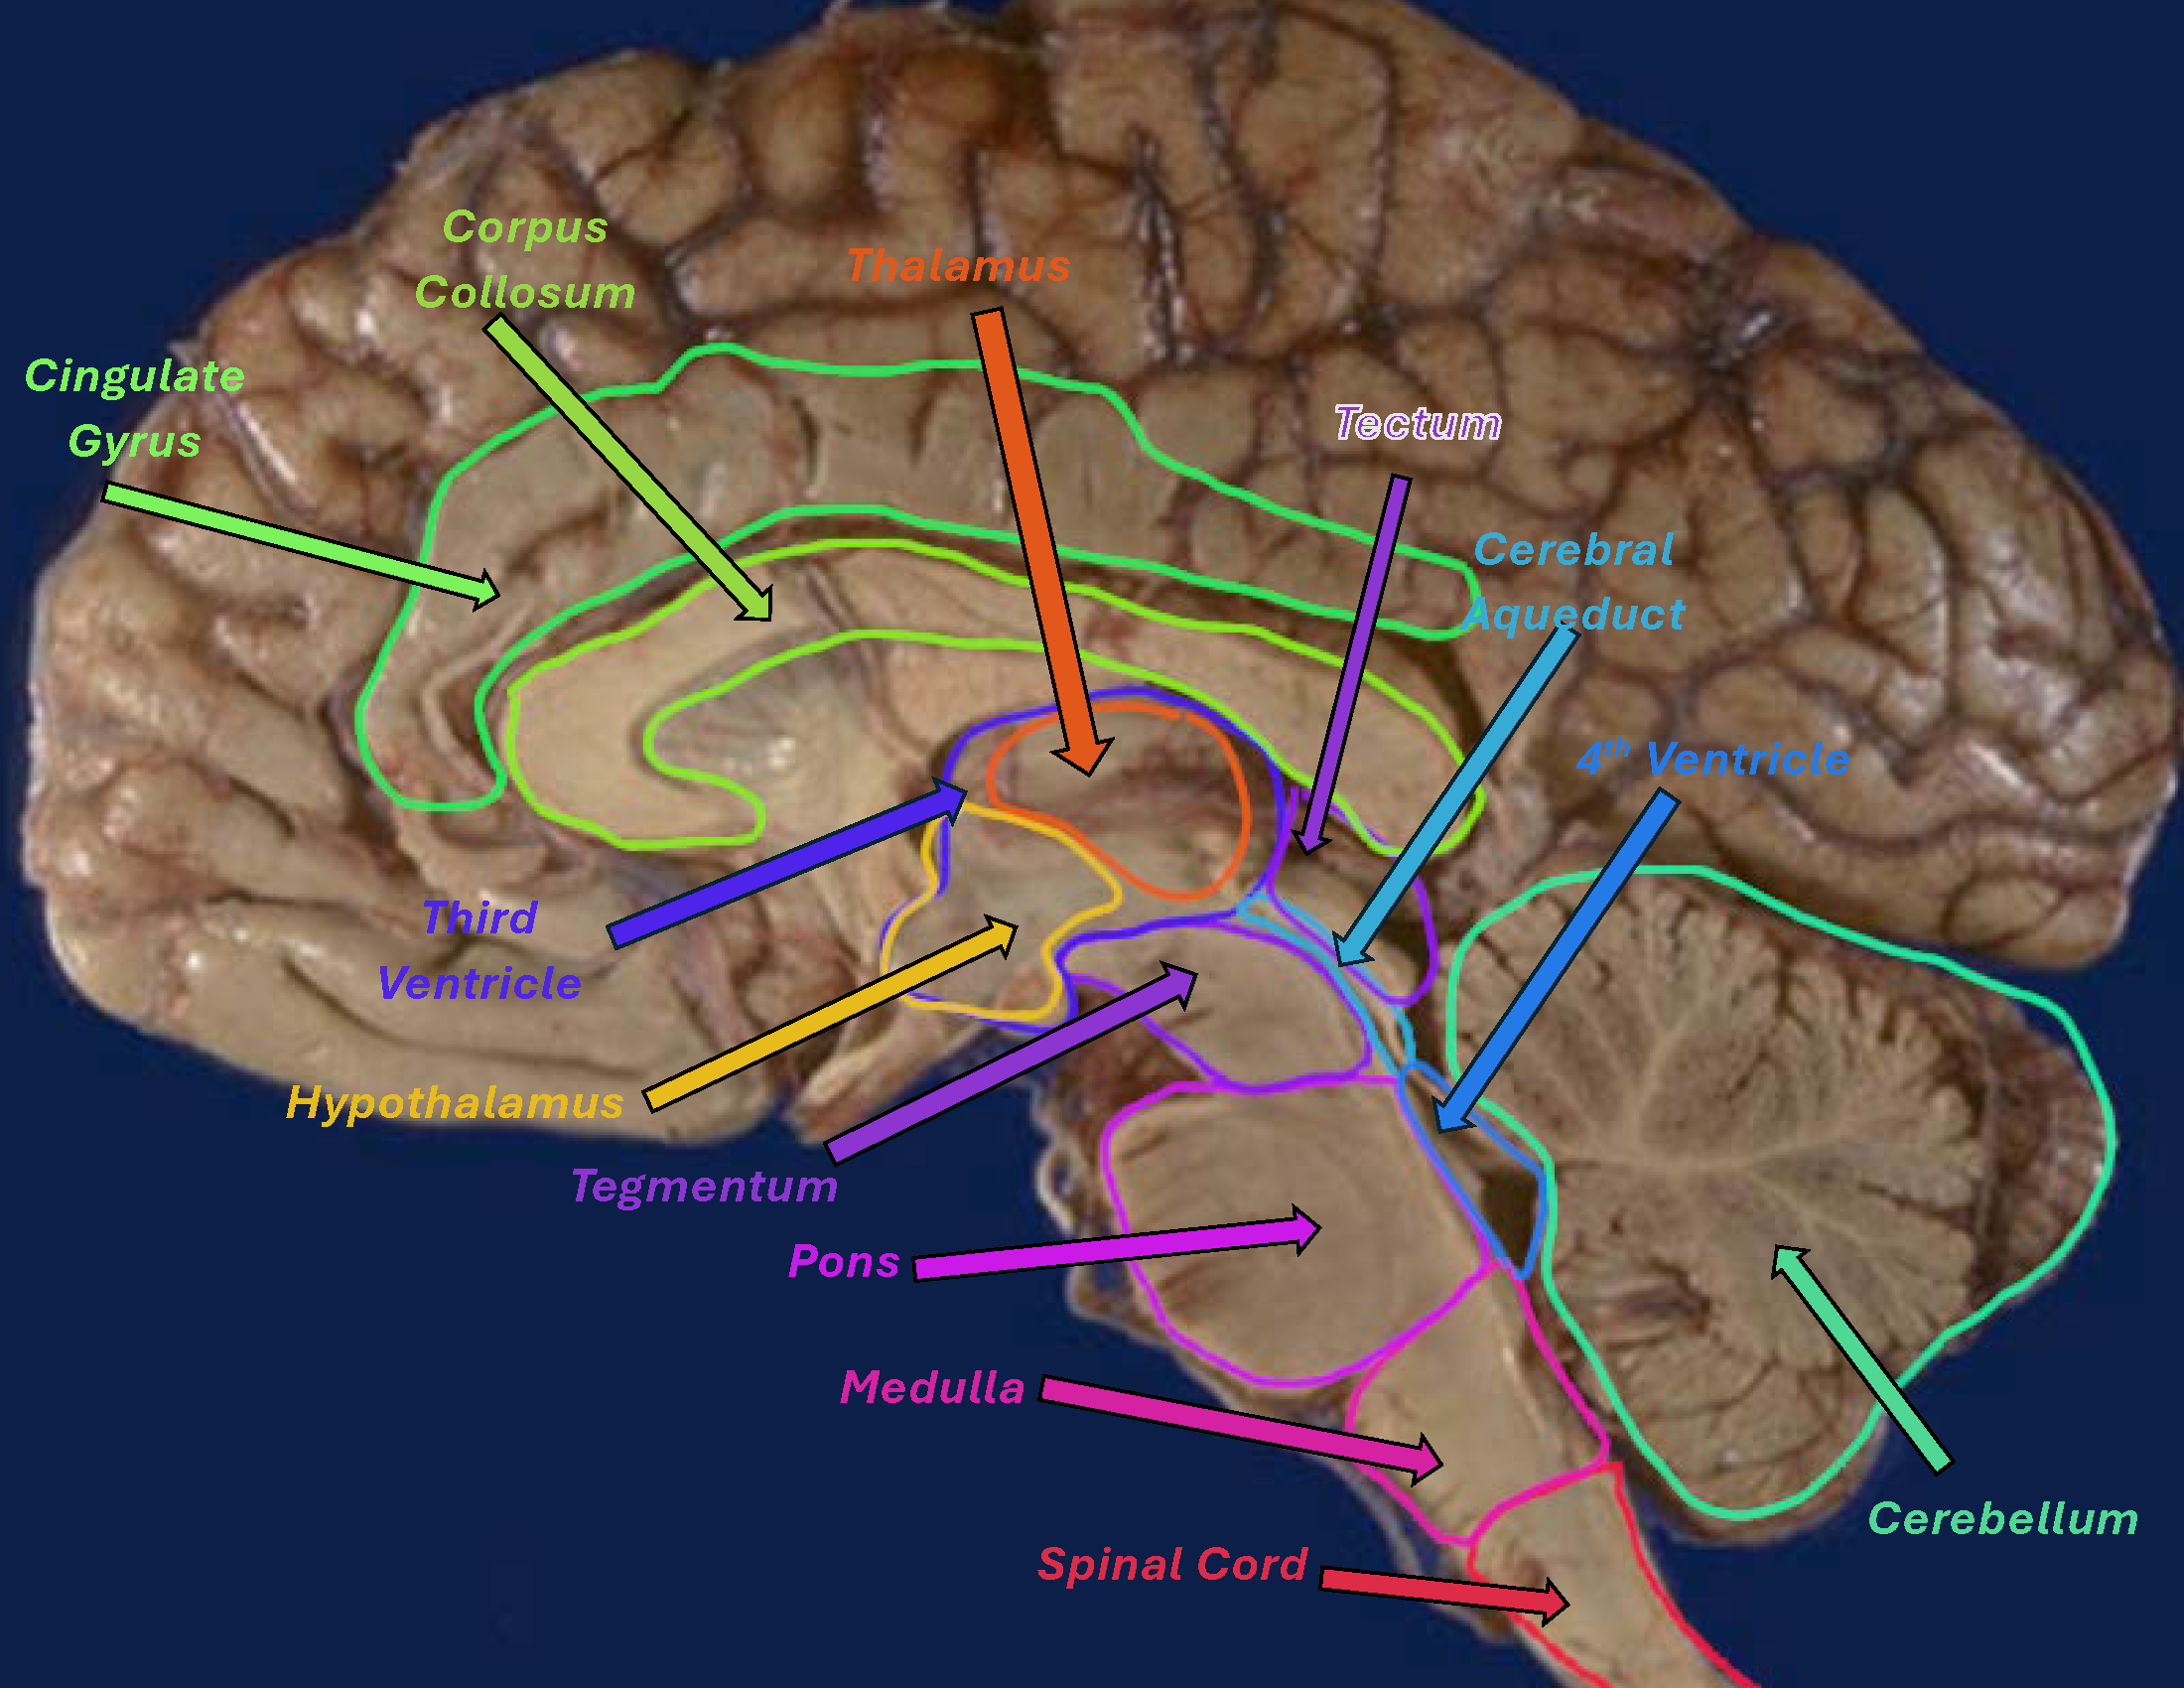
\includegraphics[width=.95\paperwidth,height=.95\paperheight,keepaspectratio]{images/midsagital_labeled.png}
%   \end{landscape}

\chapter*{Exam 1b}
\fancyhead[R]{Exam 1b}
\addcontentsline{toc}{chapter}{Exam 1b}
\vspace*{-0.25in}
% ===========================
% Section 1.1: Neuroanatomy \& Nervous System Structure
% ===========================
\section*{1.1 \squigglyline}

\textbf{Directions:} For short answer questions, write your response in the space provided. Most of the short answer questions should be only a sentence or two long. For multiple choice questions, circle the letter of the correct response. For fill-in-the-blank questions, write your response in the space provided. For matching questions, write the letter of the correct response in the space to the right. For true or false questions, write ``True'' if the statement is true, and if the statement is false, \textit{explain why} the statement is false. Lastly, the sections (1.1, 1.2, etc.) are provided to break the exam into smaller parts. Good luck!

\begin{enumerate}[label=\textbf{Q1.1.\arabic*}]
      % Short answer question
      \item \textbf{Short Answer:} Define neuroscience. \\
            \textit{Answer:} \\%The study of the nervous system.

            % T/F question
      \item \textbf{True or False:} Behavioral neuroscience involves understanding the nervous system’s underlying behavior. \\
            \textit{Answer:} %True.

% Change this question
            % Fill in the blank
      \item \textbf{Fill in the Blank:} The Central Nervous System (CNS) is composed of the \underline{\hspace{2cm}} and the \underline{\hspace{2cm}}.
            \\
            %\textit{Answer:} Brain; spinal cord.

            % Matching question
      \item \textbf{Matching:} Match the following systems with their primary functions.
            \begin{wordbox}
                  \begin{enumerate}[label=(\roman*)]
                        \item Voluntary motor control and sensory input.
                        \item Involuntary control of the gastrointestinal system.
                        \item Involuntary control of smooth muscle and glands.
                  \end{enumerate}
            \end{wordbox}
            \begin{enumerate}[label=(\alph*)]
                  \item Somatic Nervous System \quad \dotfill \quad \underline{\hspace{3cm}}\\[0.5em]
                  \item Autonomic Nervous System \quad \dotfill \quad \underline{\hspace{3cm}}\\[0.5em]
                  \item Enteric Nervous System \quad \dotfill \quad \underline{\hspace{3cm}}
            \end{enumerate}
            %\textit{Answer:} (a) Voluntary motor control and sensory input; (b) Involuntary control of smooth muscle and glands; (c) Involuntary control of the gastrointestinal system.

% Change this question
      \item \textbf{Fill in the Blank} The autonomic nervous system regulates the body's \underline{\hspace{3cm}} AND \underline{\hspace{3cm}} response. \\
            %\textit{Answer} Fight or flight; rest and digest. OR Sympathetic; parasympathetic.

% Change this question
      \item \textbf{Short Answer:} How does the flight-or-flight response affect your body? \\
            \textit{Answer:} \\%Increases Heart rate, blood pressure, respiration, and alertness.

% Change this question
      \item \textbf{Fill in the Blank:} In the fecal microbiota transplant study, researchers found that the microbiota change the \underline{\hspace{3cm}} of the mice. \\
            %\textit{Answer:} Behavior.

% Change this question
      \item \textbf{Fill in the Blank:} In the elevated plus maze study, researchers found that the anxious mice were more willing to \underline{\hspace{3cm}} after the fecal microbiota transplant. \\
            %\textit{Answer:} Walk on the open arms.
\end{enumerate}

% ===========================
% Section 1.2: Meninges
% ===========================
\section*{1.2 \squigglyline}
\begin{enumerate}[label=\textbf{Q1.2.\arabic*}]
      \item \textbf{Short Answer:} What is the primary function of the meninges? \\
            \textit{Answer:} \\%To cover and protect the nervous system.

      \item \textbf{Multiple Choice:} Which of the following is the middle meningeal layer?
            \begin{tasks}[label=(\Alph*), label-width=1.5em, item-indent=1.7em](2) % two columns 
                  \task Arachnoid Membrane
                  \task Dura Mater
                  \task Pia Mater
                  \task Subarachnoid Space
            \end{tasks}
            %\textit{Answer:} A.

% Change this question. This is too easy.
      \item \textbf{Short Answer:} Why did early anatomists call the outermost meningeal layer ``pachymenginges''? \\
            \textit{Answer:} \\%Because it was similar to elephant skin.

      \item \textbf{Fill in the Blank} The Peripheral Nervous System uses \underline{\hspace{3cm}} layer(s) of the meninges. \\
            %\textit{Answer:} Two.

      \item \textbf{Fill in the Blank:} Arachnoid \underline{\hspace{3cm}} are web-like structures that connect the Arachnoid Membrane to the \textit{pia mater}
            %\textit{Answer:} trabeculae.

% Change this question
      \item \textbf{Fill in the Blank:} The subarachnoid space is filled with \underline{\hspace{3cm}}. \\
            %\textit{Answer:} Cerebrospinal fluid.

      \item \textbf{Short Answer:} What is meningitis? \\
            \textit{Answer:} \\%Inflammation of the meninges.

% Change this question
      % Changed question: Making the question more challenging by evaluating symptom combinations.
      \item \textbf{Multiple Choice:} Which combination of symptoms is LEAST consistent with a diagnosis of acute bacterial meningitis?
            \begin{tasks}[label=(\Alph*), label-width=1.5em, item-indent=1.7em](2)
                  \task Fever, headache, and nuchal rigidity.
                  \task Photophobia, vomiting, and altered mental status.
                  \task None of the above
            \end{tasks}
            %\textit{Answer:} D.
\end{enumerate}

% ===========================
% Section 1.3: Cerebrospinal Fluid (CSF)
% ===========================
\section*{1.3 \squigglyline}
\begin{enumerate}[label=\textbf{Q1.3.\arabic*}]
      \item \textbf{Short Answer:} List two functions of CSF. \\
            \textit{Answer:} \\%Protection, transportation of neurotransmitters, waste, hormones, and nutrients.

% Change this question
      \item \textbf{True or False:} CSF is similar in composition to blood plasma. \\
            \textit{Answer:} %True.

      \item \textbf{Fill in the Blank:} CSF is produced by the \underline{\hspace{3cm}} cells lining the lateral ventricles.
            %\textit{Answer:} ependymal.

      \item \textbf{Fill in the Blank:} A contra-coup injury is an injury that occurs on the \underline{\hspace{3cm}} side of the brain from the impact site.
            %\textit{Answer:} opposite.
\end{enumerate}

% ===========================
% Section 1.4: Flow of CSF
% ===========================
\section*{1.4 \squigglyline}
\begin{enumerate}[label=\textbf{Q1.4.\arabic*}]
      \item \textbf{Matching:} Match the location with its description.
            \begin{wordbox}
                  \begin{enumerate}[label=(\roman*)]
                        \item Connected to the pituitary gland via the infundibulum.
                        \item Production of CSF and connection to the third ventricle via the interventricular foramen.
                        \item Connects the third and fourth ventricles.
                  \end{enumerate}
            \end{wordbox}
            \begin{enumerate}[label=(\alph*)]
                  \item Lateral Ventricles \quad \dotfill \quad \underline{\hspace{3cm}}\\[0.5em]
                  \item Third Ventricle \quad \dotfill \quad \underline{\hspace{3cm}}\\[0.5em]
                  \item Cerebral Aqueduct \quad \dotfill \quad \underline{\hspace{3cm}}
            \end{enumerate}
            %\textit{Answer:} (a) Production of CSF and connection to the third ventricle via the interventricular foramen; (b) Connected to the pituitary gland via the infundibulum; (c) Connects the third and fourth ventricles.

      \item \textbf{True or False:} The central canal connects the fourth ventricle to the spinal cord. \\
            \textit{Answer:} %True.
\end{enumerate}

% ===========================
% Section 1.5: Dumping of CSF
% ===========================
\section*{1.5 \squigglyline}
\begin{enumerate}[label=\textbf{Q1.5.\arabic*}]
      \item \textbf{Short Answer:} Where is CSF absorbed into the bloodstream? \\
            \textit{Answer:} \\%Through the arachnoid villi/granulations into the superior sagittal sinus.

      \item \textbf{Fill in the Blank:} \underline{\hspace{3cm}} is caused by swelling of the brain due to a blockage in the CSF flow. \\
            %\textit{Answer:} Hydrocephalus.

% Change this question to a fill in the blank or multiple choice.
      \item \textbf{True or False:} The \textit{Interventricular Foramen} connects the lateral ventricles to the third ventricle. \\
            \textit{Answer:} %True.
\end{enumerate}

% ===========================
% Section 1.6: Getting Some CSF Out -- or -- Putting Something Into It
% ===========================
\section*{1.6 \squigglyline}

\begin{enumerate}[label=\textbf{Q1.6.\arabic*}]
      
% Change this question
      \item \textbf{Fill in the Blank:} The term ``\textit{epi}'' means \underline{\hspace{3cm}} and the term ``\textit{tap}'' means \underline{\hspace{3cm}}. \\
            %\textit{Answer:} %Something in; Taking something out.

      \item \textbf{Multiple Choice:} A lumbar puncture is sometimes called a:
            \begin{tasks}[label=(\Alph*), label-width=1.5em, item-indent=1.7em](2) % two columns 
                  \task Brain Tap
                  \task Spinal Tap
                  \task CSF Drain
                  \task Ventricular Tap
            \end{tasks}
            %\textit{Answer:} %B.

      \item \textbf{Fill in the Blank:} The needle for a lumbar puncture is typically inserted into the \underline{\hspace{3cm}} sac in the lumbar region.
            \\
            %\textit{Answer:} dural.
\end{enumerate}

% ===========================
% Section 1.7: Cranial Nerves
% ===========================
\section*{1.7 \squigglyline}
\begin{enumerate}[label=\textbf{Q1.7.\arabic*}]

      \item \textbf{Matching:} Match the cranial nerve number with its function.
            \begin{wordbox}
                  \begin{enumerate}[label=(\roman*)]
                        \item Facial sensation or motor control of the mandible
                        \item Vision
                        \item Smell
                  \end{enumerate}
            \end{wordbox}
            \begin{enumerate}[label=(\alph*)]
                  \item I \quad \dotfill \quad \underline{\hspace{3cm}}\\[0.5em]
                  \item II \quad \dotfill \quad \underline{\hspace{3cm}}\\[0.5em]
                  \item V \quad \dotfill \quad \underline{\hspace{3cm}}
            \end{enumerate}
            %\textit{Answer:} (a) Olfaction (smell); (b) Vision; (c) Facial sensation or motor control of the mandible.

      \item \textbf{True or False:} Cranial nerve IV controls pupil constriction and eye movement. \\
            \textit{Answer:} %False. (It only controls eye movement. OR, the statement is true if you're talking about cranial nerve III.)

      \item \textbf{Short Answer:} What is the function of cranial nerve X? \\
            \textit{Answer:} \\ %Taste and sensation from neck, thorax, abdomen, swallowing, control of laryx, parasympathetic nerves to heart and viscera.

% Change this question
      \item \textbf{Fill in the Blank:} There are \underline{\hspace{3cm}} cranial nerve(s) that modulate eye movements, and \underline{\hspace{3cm}} cranial nerve(s) that control the sense of vision. \\
            %\textit{Answer:} %Three; one.

      \item \textbf{True or False:} The term ``\textit{glossal}'' means ``taste''. \\
            \textit{Answer:} %False. (It means tongue.)

      \item \textbf{Fill in the Blank:} For the following table, fill in the blanks with the correct name.

% Add in sensory or motor or both column.
            \begin{multicols}{2}
                  \begin{tabular}{cc}
                        \toprule
                        \textbf{Cranial Nerve} & \textbf{Name}            \\ \midrule
                        I                      & \underline{\hspace{3cm}} \\[0.5em]
                        II                     & \underline{\hspace{3cm}} \\[0.5em]
                        III                    & \underline{\hspace{3cm}} \\[0.5em]
                        IV                     & \underline{\hspace{3cm}} \\[0.5em]
                        V                      & \underline{\hspace{3cm}} \\[0.5em]
                        VI                     & \underline{\hspace{3cm}} \\[0.5em]
                        \bottomrule
                  \end{tabular}
                  \begin{tabular}{cc}
                        \toprule
                        \textbf{Cranial Nerve} & \textbf{Name}            \\ \midrule
                        VII                    & \underline{\hspace{3cm}} \\[0.5em]
                        VIII                   & \underline{\hspace{3cm}} \\[0.5em]
                        IX                     & \underline{\hspace{3cm}} \\[0.5em]
                        X                      & \underline{\hspace{3cm}} \\[0.5em]
                        XI                     & \underline{\hspace{3cm}} \\[0.5em]
                        XII                    & \underline{\hspace{3cm}} \\[0.5em]
                        \bottomrule
                  \end{tabular}
            \end{multicols}

\end{enumerate}

% ===========================
% Section 1.8: Terms
% ===========================
\section*{1.8 \squigglyline}
\begin{enumerate}[label=\textbf{Q1.8.\arabic*}]

      \item \textbf{Short Answer:} What does the term \textit{Soma} refer to? \\
            \textit{Answer:}% The cell body of a neuron.

      \item \textbf{True or False:} The term ``\textit{nucleus}'' refers to a collection of cell bodies in the PNS. \\
            \textit{Answer:} %False. (It refers to a collection of cell bodies in the CNS.)

      \item \textbf{Fill in the Blank:} Fill in the following table for the terms that match its definition. \\

            \begin{tabular}[htbp]{cc}
                  \toprule
                  \textbf{Term}            & \textbf{Definition}                           \\ \midrule
                  Tract                    & \underline{\hspace{10cm}}                     \\[0.5em]
                  \underline{\hspace{3cm}} & The ends of the neuron that send information. \\[0.5em]
                  \underline{\hspace{3cm}} & Extends surface area of the neuron.           \\[0.5em]
                  \underline{\hspace{3cm}} & A collection of axons in the PNS.             \\        \bottomrule
            \end{tabular}
            %\textit{Answer:} %A collection of axons in the CNS; axonal buttons; dendrites; nerve.

      \item \textbf{True or False:} \textit{Ganglion} are collections of axons. \\
            \textit{Answer:} %False. (They are collections of cell bodies.)

      \item \textbf{Short Answer:} What is the function of the myelin sheath? \\
            \textit{Answer:} %To insulate the axon and speed up the transmission of the action potential.
\end{enumerate}

% ===========================
% Section 1.9: Brainstem --- Hindbrain and Midbrain
% ===========================
\section*{1.9 \squigglyline}
\begin{enumerate}[label=\textbf{Q1.9.\arabic*}]
      \item \textbf{Short Answer:} Name two principal structures of the hindbrain. \\
            \textit{Answer:} \\%Medulla Oblongata and Pons (or Cerebellum).

      \item \textbf{Short Answer:} What vital functions are regulated by the Reticular Formation in the Medulla Oblongata? \\
            \textit{Answer:} \\ % Heart rate, blood pressure, respiration.

      \item \textbf{Short Answer:} Describe the role of the Pons in the brainstem. \\
            \textit{Answer:} % Acts as a bridge connecting various brain regions and houses the Locus Coeruleus.

      \item \textbf{Fill in the Blank:} Pons directly translates to \underline{\hspace{3cm}} in Latin. \\
            %\textit{Answer:} %Bridge.

      \item \textbf{Fill in the Blank:} The \underline{\hspace{3cm}} (specific) is a structure in the pons that produces norepinephrine. \\
            %\textit{Answer:} %Locus Coeruleus.

% Change this question. It directly answers the question before it.
      \item \textbf{True or False:} The norepinephrine produced by the Locus Coeruleus is sent primarily to the hind brain. \\
            \textit{Answer:} %False. (It is sent to the forebrain.)

      \item \textbf{Short Answer:} What is the primary function of the cerebellum? \\
            \textit{Answer:} %Coordination of movement and balance.

      \item \textbf{\textit{Bonus} Short Answer:} Can you name every function of the cerebellum? (There's 8!) \\
            \textit{Answer:} \\[0.5em]%Balance, hand-eye coordination, soothes movements, shifts attention between vision and hearing, sensory timing (judging rhythm), language, emotional control, and reward valuation.

      \item \textbf{Fill in the Blank:} The rare malformation wherein the cerebellum is not developed is called \underline{\hspace{3cm}}. \\
            %\textit{Answer:} %Cerebellar agenesis.

% Change this question. It is answered by a later question.
      \item \textbf{Multiple Choice:} Which of the following midbrain structures is primarily responsible for visual reflexes? \\
            (A) Olives \quad (B) Pyramids \quad (C) Superior Colliculus \quad (D) Substantia Nigra \\
            %\textit{Answer:} %C.

      \item \textbf{Fill in the Blank:} The \underline{\hspace{3cm}} in the midbrain is critical for motor coordination. \\
            %\textit{Answer:} %Red nucleus.

      \item \textbf{Short Answer:} What does the \textit{periaqueductal gray area} produce? \\
            \textit{Answer:} \\%Opioiods

% Change this question to fill in the blank.
      \item \textbf{True or False:} The medulla oblongata contains the reticular formation which regulates vital functions like heart rate and respiration. \\
            \textit{Answer:} %True.

% Change this question. It answers the question referenced before.
      \item \textbf{Fill in the Blank:} The midbrain’s \underline{\hspace{3cm}} Colliculus is important for visual reflexes, while the \underline{\hspace{3cm}} Colliculus is involved in auditory reflexes.
            % \textit{Answer:} Superior; Inferior.

      \item \textbf{Multiple Choice:} The \textit{substantia nigra} is known for its role in:
            \begin{enumerate}[label=(\Alph*)]
                  \item Serotonin production
                  \item Dopamine production
                  \item GABA production
                  \item Acetylcholine production
            \end{enumerate}
            %\textit{Answer:} %B.
\end{enumerate}

% ===========================
% Section 1.10: Forebrain --- Diencephalon and Telencephalon
% ===========================
\section*{1.10 \squigglyline}
\begin{enumerate}[label=\textbf{Q1.10.\arabic*}]
      \item \textbf{Short Answer:} What is the role of the thalamus in the brain? \\
            \textit{Answer:} %It relays sensory and motor signals

      \item \textbf{Fill in the Blank:} Fill in the following table with the correct terms.
            \begin{table}[htbp]
                  \centering
                  \begin{tabular}{cc}
                        \toprule
                        \textbf{Thalamic Relay Nuclei} & \textbf{Description} \\ \midrule
                        \underline{\hspace{3cm}}       & Vision               \\
                        \underline{\hspace{3cm}}       & Pain                 \\
                        \underline{\hspace{3cm}}       & Promotes wakefulness \\
                        \bottomrule
                  \end{tabular}
            \end{table}
            %\textit{Answer:} %Lateral Geniculate Nucleus; Dorsal Medial Nucleus; Nucleus Reticularis

% Change this question
      \item \textbf{Short Answer:} What does it mean to be a non-specific relay nuclei? \\
            \textit{Answer:} %It means that the thalamic nuclei do not have a specific function.

      \item \textbf{Multiple Choice:} The thalamic nucleus responsible for pain routing sends those signals to the:
            \begin{tasks}[label=(\Alph*), label-width=1.5em, item-indent=1.7em](2) % two columns 
                  \task Prefrontal Cortex
                  \task Primary Somatosensory Cortex
                  \task Primary Motor Cortex
                  \task Amygdala
            \end{tasks}
            %\textit{Answer:} %A.

% Either move this question to a different spot or change it.
      \item \textbf{Fill in the Blank:} The \textit{Massa Intermedia} connects the left \underline{\hspace{3cm}} half with the right half. \\
            %\textit{Answer:} %Thalamus.

      \item \textbf{Multiple Choice:} Which of the following is NOT a function of the hypothalamus?
            \begin{enumerate}[label=(\Alph*)]
                  \item Survival of the individual
                  \item Survival of the species
                  \item Regulation of endocrine system
                  \item Integration of information
            \end{enumerate}
            %\textit{Answer:} %C.



% Change this question
      \item \textbf{True or False:} The hypothalamus is involved in both individual survival functions (like eating and drinking) and species survival functions (such as reproduction). \\
            \textit{Answer:} %True.


% Change this question. Possibly multiple choice instead.
      \item \textbf{True or False:} The \textit{Suprachiasmatic Nucleus} is responsible for circadian rhythms. \\
            \textit{Answer:} %True.

% Change this question. Too easy with process of elimination.   
      \item \textbf{Matching:} Match the following telencephalic structures with their functions.
            \begin{wordbox}
                  \begin{enumerate}[label=(\roman*)]
                        \item Sensory integration and spatial awareness.
                        \item Executive functions, motor control, language production.
                        \item Memory, hearing, language comprehension.
                        \item Vision
                  \end{enumerate}
            \end{wordbox}
            \begin{enumerate}[label=(\alph*)]
                  \item Frontal Lobe \quad \dotfill \quad \underline{\hspace{3cm}}\\[0.5em]
                  \item Temporal Lobe \quad \dotfill \quad \underline{\hspace{3cm}}\\[0.5em]
                  \item Parietal Lobe \quad \dotfill \quad \underline{\hspace{3cm}}\\[0.5em]
                  \item Occipital Lobe \quad \dotfill \quad \underline{\hspace{3cm}}
            \end{enumerate}
            %\textit{Answer:} (a) Executive functions, motor control, language production; (b) Memory, hearing, language comprehension; (c) Sensory integration and spatial awareness. (d) Vision.

      \item \textbf{Fill in the Blank:} The \textit{Corpus Callosum}'s neurons go from \underline{\hspace{3cm}} to \underline{\hspace{3cm}} and not from \underline{\hspace{3cm}} to \underline{\hspace{3cm}}. (Your answers should directions.) \\
            %\textit{Answer:} %Lateral to lateral; dorsal to ventral.

      \item \textbf{Multiple Choice:} Which of the following is NOT a symptom of Callosal Agenesis?
            \begin{tasks}[label=(\Alph*), label-width=1.5em, item-indent=1.7em](2) % two columns 
                  \task Impaired motor coordination
                  \task Impaired language comprehension
                  \task Impaired spatial awareness
                  \task Impaired executive functions
            \end{tasks}
            %\textit{Answer:} %B.

      \item \textbf{Fill in the Blank:} The \underline{\hspace{3cm}} is involved in the regulation of voluntary motor control. \\
            %\textit{Answer:} %Basal Ganglia.

      \item \textbf{Fill in the Blank:} The \textit{Striatum} consists of the \underline{\hspace{3cm}}, \underline{\hspace{3cm}}, and the \underline{\hspace{3cm}}. (\textit{Note:} The \textit{Globus Pallidus} is not a viable answer here.) \\
            %\textit{Answer:} %Caudate Nucleus; Putamen, Nucleus accumbens.

      \item \textbf{True or False:} When people mention the Nucleus Accumbens and the Globus Pallidus, they call it the lentiform nucleus. \\
            \textit{Answer:} %False. (The putamen and the globus pallidus are called the lentiform nucleus.)

      \item \textbf{Fill in the Blank:} Participants in Rees et al.'s (2011) study showed extreme conservatives had a larger \underline{\hspace{3cm}} \\
            %\textit{Answer:} %Amygdala.

      \item \textbf{Short Answer:} How does the hippocampus have an impact upon memory? \\
            \textit{Answer:} %Moves memories from short-term to long-term storage.

      \item \textbf{Short Answer:} What is the left hemisphere of the brain responsible for? And the right hemisphere? (2 each.) \\
            \textit{Answer:} \\%Left: Language, serial events; Right: Creativity, synthesis of information. 

      \item \textbf{Matching:} Arrange the following structures in the brain in the right order.
      \begin{wordbox}
            \begin{enumerate}[label=(\roman*)]
                  \item Tectum
                  \item Medulla Oblogata
                  \item Limbic System
                  \item Hypothalamus
            \end{enumerate}
      \end{wordbox}
      \begin{enumerate}[label=(\alph*)]
            \item Myelencephalon \quad \dotfill \quad \underline{\hspace{3cm}}\\[0.5em]
            \item Diencephalon \quad \dotfill \quad \underline{\hspace{3cm}}\\[0.5em]
            \item Telencephalon \quad \dotfill \quad \underline{\hspace{3cm}}\\[0.5em]
            \item Mesencephalon \quad \dotfill \quad \underline{\hspace{3cm}}\\
      \end{enumerate}
      %\textit{Answer:} %B, D, C, A.

      \item \textbf{Short Answer:} What is \textit{Kluver-Bucy Syndrome}? \\
            \textit{Answer:} %A condition where the amygdala is damaged, leading to loss of normal fear and anger responses.

      \item \textbf{Fill in the Blank:} The \underline{\hspace{3cm}} is involved in the regulation of emotions, memory, and motivation. \\
            %\textit{Answer:} %Limbic System.

      \item \textbf{Fill in the Blank:} Selective attention, love, and pain are all functions of the \underline{\hspace{3cm}}. \\
            %\textit{Answer:} %Cingulate gyrus.

      \item \textbf{Short Answer:} What lobes make up the \textit{Cerebral Cortex}? \\
            \textit{Answer:} \\%Frontal, Parietal, Temporal, Occipital.

      \item \textbf{Short Answer:} We learned that the \textit{Temporal Lobe} is responsible for language comprehension. Who was the scientist that discovered this? Similarly, we learned that the \textit{Frontal Lobe} is responsible for language production. Who was the scientist that discovered this? \\
            \textit{Answer:} \\%Wernicke; Broca.

      \item \textbf{Multiple Choice:} In a study by Eisenberger (1990) called the Cyberball study, participants who were excluded from the game showed increased activity in the:
            \begin{tasks}[label=(\Alph*), label-width=1.5em, item-indent=1.7em](2) % two columns 
                  \task Amygdala
                  \task Hippocampus
                  \task Anterior Cingulate Cortex
                  \task Septal Nucleus
            \end{tasks}
            %\textit{Answer:} %C.

      \item \textbf{Fill in the Blank:} Fill out the following table with the correct terms.
\end{enumerate}

\begin{table}[ht]
      \centering
      \begin{tabular}{l l l l}
            \toprule
            \textbf{Major Divisions} & \textbf{Ventricle}                                       & \textbf{Subdivision}          & \textbf{Principal Structures} \\
            \midrule

            %--- Forebrain Block ----------------------------------
            \multirow{7}{*}{Forebrain}
                                     & \multirow{5}{*}{\underline{\hspace{3cm}}}
                                     & \multirow{4}{*}{\underline{\hspace{3cm}}}
                                     & \underline{\hspace{3cm}}                                                                                   \\
                                     &                                                          &
                                     & \underline{\hspace{3cm}}                                                                                   \\
                                     &                                                          &
                                     & \underline{\hspace{3cm}}                                                                                     \\
                                     &                                                          &
                                     & \underline{\hspace{3cm}}                                                                                     \\[0.5em]
            \cline{3-4}                                                                                                                                         \\[-0.5em]
                                     & \multirow{2}{*}{\underline{\hspace{3cm}}}             & \multirow{2}{*}{\underline{\hspace{3cm}}}
                                     & \underline{\hspace{3cm}}                                                                                          \\
                                     &                                                          &
                                     & \underline{\hspace{3cm}}                                                                                      \\
            \midrule

            %--- Midbrain Block ------------------------------------
            \multirow{4}{*}{Midbrain}
                                     & \multirow{4}{*}{\underline{\hspace{3cm}}}
                                     & \multirow{4}{*}{\underline{\hspace{3cm}}}
                                     & \underline{\hspace{3cm}}                                                                                             \\
                                     &                                                          &
                                     & \underline{\hspace{3cm}}                                                                                         \\
                                     &                                                          &
                                     & \underline{\hspace{3cm}}                                                                               \\
                                     &                                                          &
                                     & \underline{\hspace{3cm}}                                                                               \\
            \midrule

            %--- Hindbrain Block -----------------------------------
            \multirow{4}{*}{Hindbrain}
                                     & \multirow{4}{*}{\underline{\hspace{3cm}}}
                                     & \multirow{2}{*}{\underline{\hspace{3cm}}}
                                     & \underline{\hspace{3cm}}                                                                                        \\
                                     &                                                          &
                                     & \underline{\hspace{3cm}}                                                                                               \\[0.5em]
            \cline{3-4}                                                                                                                                         \\[-0.5em]
                                     &                                                          & \underline{\hspace{3cm}}
                                     & \underline{\hspace{3cm}}                                                                                 \\
            \bottomrule
      \end{tabular}
      \label{tab:brain-divisions}
\end{table}

% ===========================
% Section 1.11: Parkinson's and Alzheimer's Disease
% ===========================
\section*{1.11 \squigglyline}
\begin{enumerate}[label=\textbf{Q1.11.\arabic*}]
      \item \textbf{Multiple Choice:} Which of the following is NOT a typical symptom of Parkinson's Disease? \\
            (A) Bradykinesia \quad (B) Rigidity \quad (C) Tremors \quad (D) Hyperactivity
            %\textit{Answer:} %D

      \item \textbf{Short Answer:} Name one symptom associated with Alzheimer's Disease. \\
            \textit{Answer:} %Progressive memory loss.

      \item \textbf{True or False:} Only retrograde amnesia is observed in Alzheimer's Disease. \\
            \textit{Answer:} %False. (Both retrograde and anterograde amnesia are observed.)
\end{enumerate}


% \chapter*{Exam 2}
% \fancyhead[R]{Exam 2}
% \addcontentsline{toc}{chapter}{Exam 2}
% \vspace*{-0.25in}
% % ===========================
% Section 2.1 -- The Neuron
% ===========================
\section*{2.1}
\begin{enumerate}[label=\textbf{Q2.1.\arabic*}]
      \item \textbf{Short Answer:} Define a neuron. \\
            % \textit{Answer:} Basic information processing unit of the nervous system.
      \item \textbf{Multiple Choice:} Which cell type forms the myelin sheath in the CNS?
            \begin{tasks}[label=\textcolor{draculafg}{(\Alph*)}, item-format=\color{draculafg}, label-width=1.5em, item-indent=1.7em](2)
                  \task Oligodendrocytes
                  \task Schwann Cells
                  \task Astrocytes
                  \task Satellite Cells
            \end{tasks}
            % \textit{Answer:} A
      \item \textbf{Fill in the Blank:} The process by which glial cells remove debris is called \underline{\hspace{3cm}}. \\
            % \textit{Answer:} Phagocytosis.
      \item \textbf{Short Answer:} Name two functions of astrocytes. \\
            % \textit{Answer:} Provide structural support and deliver nutrients to neurons.
      \item \textbf{Fill in the Blank:} \underline{\hspace{3cm}} are responsible for myelination in the PNS. \\
            % \textit{Answer:} Schwann Cells.
      \item \textbf{Multiple Choice:} What is one function of myelin?
            \begin{tasks}[label=\textcolor{draculafg}{(\Alph*)}, item-format=\color{draculafg}, label-width=1.5em, item-indent=1.7em](2)
                  \task Insulate axons
                  \task Synthesize proteins
                  \task Produce neurotransmitters
                  \task Break down debris
            \end{tasks}
            % \textit{Answer:} A.
      \item \textbf{Fill in the Blank:} Glial cells compose about half of nervous tissue volume, but are approximately \underline{\hspace{3cm}} times more numerous than neurons. \\
            % \textit{Answer:} 10-50.

      \item \textbf{Short Answer:} What are two similarities between neurons and other animal cells? \\
            % \textit{Answer:} They have a cell membrane, a nucleus, and a variety of organelles.
      \item \textbf{Short Answer:} In neurons, what is the primary role of mitochondria? \\
            % \textit{Answer:} Producing energy for the cell.
      \item \textbf{Fill in the Blank:} The organelle responsible for protein synthesis in neurons is the \underline{\hspace{3cm}}. \\
            % \textit{Answer:} Endoplasmic Reticulum.
      \item \textbf{Fill in the Blank:} The \underline{\hspace{3cm}} packages neurotransmitters for transport. \\
            % \textit{Answer:} Golgi Apparatus.
      \item \textbf{Fill in the Blank:} Organelles that break down waste products in neurons are called \underline{\hspace{3cm}}. \\
            % \textit{Answer:} Lysosomes.
      \item \textbf{Short Answer:} What distinguishes the morphology of neurons from typical animal cells? \\
            % \textit{Answer:} Neurons have long processes (axons and dendrites) specialized for signal transmission.
      \item \textbf{Fill in the Blank:} Neurons communicate via an \underline{\hspace{3cm}} process. \\
            % \textit{Answer:} electrochemical.
      \item \textbf{Multiple Choice:} Which cell type is primarily responsible for debris removal in the CNS?
            \begin{tasks}[label=\textcolor{draculafg}{(\Alph*)}, item-format=\color{draculafg}, label-width=1.5em, item-indent=1.7em](2)
                  \task Microglia
                  \task Astrocytes
                  \task Oligodendrocytes
                  \task Satellite Cells
            \end{tasks}
            % \textit{Answer:} A.
      \item \textbf{Multiple Choice:} Which cells line the ventricles and help form CSF?
            \begin{tasks}[label=\textcolor{draculafg}{(\Alph*)}, item-format=\color{draculafg}, label-width=1.5em, item-indent=1.7em](2)
                  \task Astrocytes
                  \task Ependymal Glia
                  \task Schwann Cells
                  \task Microglia
            \end{tasks}
            % \textit{Answer:} B.
      \item \textbf{Short Answer:} What is the function of satellite cells in the PNS? \\
            % \textit{Answer:} They provide nutrients and physical support to neurons.

      \item \textbf{Multiple Choice:} Which glial cell in the PNS is notably associated with neuronal regeneration?
            \begin{tasks}[label=\textcolor{draculafg}{(\Alph*)}, item-format=\color{draculafg}, label-width=1.5em, item-indent=1.7em](2)
                  \task Oligodendrocytes
                  \task Microglia
                  \task Satellite Cells
                  \task Schwann Cells
            \end{tasks}
            % \textit{Answer:} D.

      \item \textbf{Multiple Choice:} What happens during maintenance of internal consistency?
            \begin{tasks}[label=\textcolor{draculafg}{(\Alph*)}, item-format=\color{draculafg}, label-width=1.5em, item-indent=1.7em](1)
                  \task Microglia remove cellular debris.
                  \task Oligodendrocytes myelinate axons.
                  \task Astrocytes absorb excess potassium ions.
                  \task Schwann cells provide nutrients to neurons.
            \end{tasks}
            % \textit{Answer:} C.
      \item \textbf{Long Answer:} What evidence supports the notion that glial cells' malfunctioning may be contributing to Alzheimer's Disease? (Your answer must include beta amyloid, Tau, and the possible cause of Alzheimer's Disease.) \\
            % \textit{Answer:} Glial cells normally remove beta amyloid plaques, but if it builds up too much outside the cell, Tau builds up inside the cell. This leads to inflammation, which may be the problem of Alzheimer's Disease.

\end{enumerate}
\newpage
\squigglyline
% ===========================
% Section 2.2 Different Kinds of Neurons
% ===========================

\section*{2.2}
\begin{enumerate}[label=\textbf{Q2.2.\arabic*}]

      \item \textbf{Fill in the Blank:} The three structural classifications of neurons are \underline{\hspace{3cm}}, \underline{\hspace{3cm}}, and \underline{\hspace{3cm}}. \\
            % \textit{Answer:} Unipolar; Bipolar; Multipolar.



      \item \textbf{Fill in the Blank:} Neurons are based on \underline{\hspace{3cm}} and \underline{\hspace{3cm}}. \\
            % \textit{Answer:} Structure; function.


      \item \textbf{Fill in the Blank:} Sensory neurons carry information from the \underline{\hspace{3cm}} to the \underline{\hspace{3cm}}. \\
            % \textit{Answer:} PNS; CNS.

      \item \textbf{Short Answer:} What is the primary function of motor neurons? \\
            % \textit{Answer:} To carry information from the CNS to muscles and glands.

      \item \textbf{Multiple Choice:} What does ``Efferent'' mean?
            \begin{tasks}[label=\textcolor{draculafg}{(\Alph*)}, item-format=\color{draculafg}, label-width=1.5em, item-indent=1.7em](4)
                  \task Incoming
                  \task Sensory
                  \task Motor
                  \task Outgoing
            \end{tasks}
            % \textit{Answer:} D.

\end{enumerate}
\squigglyline

% ===========================
% Section 2.3 Neural Communication
% ===========================

\section*{2.3}
\begin{enumerate}[label=\textbf{Q2.3.\arabic*}]


      \item \textbf{Short Answer:} What are the 2 systems of neuronal communication? \\
            % \textit{Answer:} Binary and analogue

      \item \textbf{Fill in the Blank:} A stronger-than-normal stimulus is required to cause another action potential during the \underline{\hspace{3cm}} because of hyperpolarization. \\
            % \textit{Answer:} Relative refractory period.

      \item \textbf{Fill in the Blank:} The \textit{phospholipid bilayer} is made up of \underline{\hspace{3cm}} and \underline{\hspace{3cm}}. \\
            % \textit{Answer:} Hydrophilic heads; hydrophobic tails.

      \item \textbf{Fill in the Blank:} The period during which no amount of stimulation can cause another action potential is called the \underline{\hspace{3cm}}. \\
            % \textit{Answer:} Absolute refractory period.

      \item \textbf{Short Answer:} What is \textit{diffusion}? What else is it also known as? \\
            % \textit{Answer:} The movement of ions from high to low concentration; also known as the concentration gradient.

      \item \textbf{Short Answer:} What is the threshold of excitation, and what happens when it is reached? \\
            % \textit{Answer:} The threshold of excitation is +15 mV. When it is reached, an action potential is generated.

\newpage

      \item \textbf{Matching:} Match the following terms with their definitions.
            \begin{wordbox}
                  \begin{enumerate}
                        \item Ions move toward the opposing charge.
                        \item The charge the ion ``prefers'' to be at.
                        \item Cell is resistant to reexciation for some time after AP.
                        \item The cell membrane is more open to some ions than others.
                        \item \(-70\) mV (relative to outside).
                        \item The overshoot of negative voltage after an AP.
                        \item Costs 1 ATP. 
                        \item The phase where there is a jump in voltage after \(+15\) mV is reached.
                        \item The minimum amount needed to generate an action potential. (\(+15\) mV)
                        \item \underline{\hspace{10cm}} \\
                        \textit{Answer:} (for repolarization) the cell's charge declines. 
                  \end{enumerate}
            \end{wordbox}
            \begin{enumerate}[label=(\arabic*)]
                  \item Differential Permeability \quad \dotfill \quad \underline{\hspace{1cm}} \\
                  \item Resting Membrane Potential \quad \dotfill \quad \underline{\hspace{1cm}}\\
                  \item Threshold of Excitation \quad \dotfill \quad \underline{\hspace{1cm}}\\
                  \item Depolarization \quad \dotfill \quad \underline{\hspace{1cm}}\\
                  \item Repolarization \quad \dotfill \quad \underline{\hspace{1cm}}\\
                  \item Hyperpolarization \quad \dotfill \quad \underline{\hspace{1cm}}\\
                  \item Electrostatic Pressure \quad \dotfill \quad \underline{\hspace{1cm}}\\
                  \item Equilibrium Potential \quad \dotfill \quad \underline{\hspace{1cm}}\\
                  \item Sodium Potassium Pump \quad \dotfill \quad \underline{\hspace{1cm}}\\
                  \item Refractory Period \quad \dotfill \quad \underline{\hspace{1cm}}
            \end{enumerate}
            % \textit{Answers:} 1. d; 2. e; 3. i; 4. h; 5. j; 6. f; 7. a; 8. b; 9. g; 10. c. 
      \newpage

      

      \item \textbf{Fill in the Blank:} Fill out the following diagram of the resting membrane potential of a neuron. Draw the size of each and permeability ion to ``scale'', and draw the diffusion and electric arrows with the appropriate directions. \\

      % \begin{tikzpicture}
      %       % Labels for compartments
      %       \node at (-3,4.3) {\large \textbf{\underline{In}}};
      %       \node at (3,4.3) {\large \textbf{\underline{Out}}};
      %       \node at (-5.9,4.3) {\large \textbf{\underline{Permeability}}};
          
      %     %   % Draw compartments as boxes
      %     %   \draw (-5,-4) rectangle (-1,4); % Inside compartment
      %     %   \draw (1,-4) rectangle (5,4);   % Outside compartment
          
      %       % Draw the membrane as a double line:
      %       % Left (solid) side denotes the negative (inside) and right (dotted) side the positive (outside)
      %       \draw[line width=1pt] (0.1,-4) -- (0.1,4);  
      %       \draw[dotted, line width=1pt] (-0.1,-4) -- (-0.1,4);
          
      %       % Place ion symbols on the "in" side (left) with relative sizes.
      %       % Here, potassium is large since it is more prevalent on the inside.
      %       \node (K_in) at (-3,2.5) {\huge \(\text{K}^{+}\)};
      %       \node (Na_in) at (-3,0) {\normalsize \(\text{Na}^{+}\)};
      %       \node (Cl_in) at (-3,-2.5) {\normalsize \(\text{Cl}^{-}\)};
          
      %       \node (P_K) at (-5.9,2.5) {\huge \(\text{P}\phantom{^{+}}\)};
      %       \node (P_K) at (-5.9,0) {\tiny \(\text{P}\phantom{^{+}}\)};
      %       \node (P_K) at (-5.9,-2.5) {\Large \(\text{P}\phantom{^{-}}\)};
          
      %       % Place ion symbols on the "out" side (right)
      %       % Here, sodium is made larger, etc.
      %       \node (K_out) at (3,2.5) {\normalsize \(\text{K}^{+}\)};
      %       \node (Na_out) at (3,0) {\huge \(\text{Na}^{+}\)};
      %       \node (Cl_out) at (3,-2.5) {\Large \(\text{Cl}^{-}\)};
          
      %       % Create nodes on the membrane for arrow connections
      %       \node (mem2_left) at (-0.5,0) {};
      %       \node (mem3_left) at (1.5,-2.5) {};
      %       \node (mem3_right) at (-1.5,-2.5) {};
          
      %       % Define arrow styles:
      %       \tikzset{
      %         diffusion/.style={->, >=Stealth, line width = 2pt, red},
      %         electric/.style={->, >=Stealth, line width = 2pt, blue}
      %       };
          
      %       % For each ion on the inside, draw two arrows (curved differently) going from the ion to the membrane.
      %       % The differences in the bending (and thus length) illustrate different magnitudes.
      %       % --- For K_in:
      %       \draw[electric, bend right=15] (K_in) to (K_out);
      %       \draw[diffusion, bend right=15, line width = 6pt] (K_out) to (K_in);
      %       % --- For Na_in:
      %       \draw[electric, bend left=15] (Na_out) to (mem2_left);
      %       \draw[diffusion, bend right=15] (Na_out) to (mem2_left);
      %       % --- For Cl_in:
      %       \draw[electric, bend right=15] (Cl_in) to (mem3_left);
      %       \draw[diffusion, bend right=15] (Cl_out) to (mem3_right);
          
      %       % Add a legend (key) to denote arrow styles.
      %       \node[draw, rectangle, right=1cm of K_out] (legend) {
      %         \begin{tabular}{ll}
      %           \textbf{Key:} & \\
      %           \tikz{\draw[diffusion, ->, >=Stealth, thick, red] (0,0) -- (1,0);} & Diffusion \\
      %           \tikz{\draw[electric, ->, >=Stealth, thick, blue] (0,0) -- (1,0);} & Electric \\
      %         \end{tabular}
      %       };
      % \end{tikzpicture}
            
            \begin{tikzpicture}
                  % Labels for compartments
                  \node at (-2,4.3) {\large \textbf{\underline{In}}};
                  \node at (2,4.3) {\large \textbf{\underline{Out}}};
                  \node at (-5.9,4.3) {\large \textbf{\underline{Permeability}}};

                  %   % Draw compartments as boxes
                  %   \draw (-5,-4) rectangle (-1,4); % Inside compartment
                  %   \draw (1,-4) rectangle (5,4);   % Outside compartment

                  % Draw the membrane as a double line:
                  % Left (solid) side denotes the negative (inside) and right (dotted) side the positive (outside)
                  \draw[line width=1pt] (0.1,-4) -- (0.1,4);
                  \draw[dotted, line width=1pt] (-0.1,-4) -- (-0.1,4);

                  % Place ion symbols on the "in" side (left) with relative sizes.
                  % Here, potassium is large since it is more prevalent on the inside.
                  \node (K_in) at (-2,2.5) {\huge \underline{\phantom{K}}};
                  \node (Na_in) at (-2,0) {\huge \underline{\phantom{K}}};
                  \node (Cl_in) at (-2,-2.5) {\huge \underline{\phantom{K}}};

                  \node (P_K) at (-5.9,2.5) {\huge \underline{\phantom{K}}};
                  \node (P_K) at (-5.9,0) {\huge \underline{\phantom{K}}};
                  \node (P_K) at (-5.9,-2.5) {\huge \underline{\phantom{K}}};

                  % Place ion symbols on the "out" side (right)
                  % Here, sodium is made larger, etc.
                  \node (K_out) at (2,2.5) {\huge \underline{\phantom{K}}};
                  \node (Na_out) at (2,0) {\huge \underline{\phantom{K}}};
                  \node (Cl_out) at (2,-2.5) {\huge \underline{\phantom{K}}};

                  % Create nodes on the membrane for arrow connections
                  \node (mem2_left) at (-0.5,0) {};
                  \node (mem3_left) at (1.5,-2.5) {};
                  \node (mem3_right) at (-1.5,-2.5) {};

                  % Define arrow styles:
                  \tikzset{
                        diffusion/.style={->, >=Stealth, line width = 2pt, red},
                        electric/.style={->, >=Stealth, line width = 2pt, blue}
                  };

                  % Add a legend (key) to denote arrow styles.
                  \node[draw, rectangle, right=1cm of K_out] (legend) {
                        \begin{tabular}{ll}
                              \textbf{Key:} &           \\
                                            & Diffusion \\
                                            & Electric  \\
                        \end{tabular}
                  };
            \end{tikzpicture}

      \item \textbf{Short Answer:} Why don't the \(\text{Na}^{+}\) channels reopen during repolarization? (Question directly from notes.) \\
            % \textit{Answer:} Because of the refractory period.

      \item \textbf{Multiple Choice:} During which phase of the action potential is a neuron unable to fire another action potential, no matter how strong the stimulus?
            \begin{tasks}[label=\textcolor{draculafg}{(\Alph*)}, item-format=\color{draculafg}, label-width=1.5em, item-indent=1.7em](2)
                  \task Depolarization
                  \task Repolarization
                  \task Absolute refractory period
                  \task Relative refractory period
            \end{tasks}
            % \textit{Answer:} C.

      \item \textbf{Multiple Choice:} How can an all-or-none action potential signal convey information about stimulus intensity?
            \begin{tasks}[label=\textcolor{draculafg}{(\Alph*)}, item-format=\color{draculafg}, label-width=1.5em, item-indent=1.7em](1)
                  \task By increasing the amplitude of the action potentials
                  \task By decreasing the duration of action potentials
                  \task By changing the direction of action potentials
                  \task By increasing the frequency of action potentials
            \end{tasks}
            % \textit{Answer:} D.

      \item \textbf{Short Answer:} What are equilibrium values? \\
            % \textit{Answer:} It is the voltage at which the ion’s driving force in equals the driving force out.

      \item \textbf{Fill in the Blank:} The ratio of Na\(^{+}\) to K\(^{+}\) for the sodium-potassium pump is \underline{\hspace{0.5cm}} out for \underline{\hspace{0.5cm}} in. \\
            % \textit{Answer:} 3:2.

      \item \textbf{Short Answer:} What happens in a failed attempt at an action potential? \\
            % \textit{Answer:} The threshold is not reached; the membrane potential may change slightly but returns to -70 mV.

      \item \textbf{Short Answer:} What role does electrostatic pressure play in neuronal membrane potential? \\
            % \textit{Answer:} It drives ions toward the opposing charge, aiding in establishing the RMP.
% Make this multiple choice
      \item \textbf{Fill in the Blank:} The equilibrium values for K\(^{+}\) and Na\(^{+}\) are \underline{\hspace{0.5cm}} mV and \underline{\hspace{0.5cm}} mV, respectively. \\
            % \textit{Answer:} -80 mV; +55 mV. (I found a \href{https://www.ncbi.nlm.nih.gov/books/NBK538338/#:~:text=Since%20the%20plasma%20membrane%20at%20rest%20has,than%20it%20is%20for%20Na+%20(+65%20mV).}{paper online} that said -90 mV and +65 mV, respectively, so I don't know if these are correct.)

      \item \textbf{Short Answer:} \textit{Saltatory conduction} is the process of action potentials ``jumping'' from node to node. Why do people describe this process as ``jumping''? \\
            % \textit{Answer:} Because the action potential is regenerated only at each node, so it appears to jump along the axon. 

      \item \textbf{Short Answer:} What is the resting membrane potential (RMP) of a neuron and what does it represent? \\ 
            % \textit{Answer:} \(-70\) mV; it represents the voltage difference between the inside and outside of the cell at rest.

      \item \textbf{Short Answer:} What is meant by semipermeability in the context of the cell membrane? \\
            % \textit{Answer:} Only molecules that are lipid, lipid soluble, small, and neutral can cross the membrane.

      \item \textbf{Short Answer:} List the four main functions of embedded proteins in the cell membrane. \\
            % \textit{Answer:} They function as receptors, channels (including gated channels), pumps, and enzymes.

      \item \textbf{Multiple Choice:} Differential permeability says that this ion is more permeable than others. 
      \begin{tasks}[label=\textcolor{draculafg}{(\Alph*)}, item-format=\color{draculafg}, label-width=1.5em, item-indent=1.7em](4)
            \task Na\(^{+}\)
            \task K\(^{+}\)
            \task Cl\(^{-}\)
            \task Ca\(^{2+}\)
      \end{tasks}
      % \textit{Answer: B.}

      \item \textbf{Short Answer:} How does diffusion contribute to the RMP? \\
      % \textit{Answer:} Ions move from high to low concentration across the membrane.

      \item \textbf{Multiple Choice:} What is the rate law? 
            \begin{tasks}[label=\textcolor{draculafg}{(\Alph*)}, item-format=\color{draculafg}, label-width=1.5em, item-indent=1.7em](1)
                  \task The speed at which a neuron conducts an action potential along its axon.
                  \task The time delay between the onset of a stimulus and the initiation of an action potential.
                  \task The relationship between the amplitude of an action potential and the strength of the stimulus.
                  \task Variations in the intensity of a stimulus are represented by the rate of action potentials.
                  \task None of the above.
            \end{tasks}
            % \textit{Answer: D.}


      \newpage 

      \item \textbf{Matching:} For the diagram below, identify the processes of an action potential at each labeled phase.


            \begin{tikzpicture}[scale=1.2]

                  % Draw axes
                  \draw[->, thick] (0,-4) -- (7,-4) node[right] {Time (ms)};
                  \draw[->, thick] (0,-4) -- (0,3) node[above] {Voltage (mV)};

                  % y-axis ticks and labels (scaling: 1 unit = 20 mV)
                  \foreach \y/\label in {-3.5/{-70},-2.5/{-55}, -2/{-40}, -1/{-20}, 0/{0}, 1/{20}, 2/{40}} {
                  \draw (0,\y) -- (-0.2,\y) node[left] {\label};
                  }

                  % x-axis ticks
                  \foreach \x in {0,1,2,3,4,5,6} {
                              \draw (\x,-4) -- (\x,-4.15) node[below] {\x};
                        }

                  % Draw action potential waveform using coordinates:
                  % Points (x, y) where y = mV/20:
                  % (0,-3.5):   Rest (-70 mV)
                  % (1,-3.5):   Rest
                  % (2,-2.75):  Threshold (-55 mV, since -55/20 = -2.75)
                  % (3,2):      Peak depolarization (+40 mV, 40/20 = 2)
                  % (4,-0.5):   Repolarization (-10 mV, -10/20 = -0.5)
                  % (5,-4):     Hyperpolarization (-80 mV, -80/20 = -4)
                  % (6,-3.5):   Return to rest (-70 mV)
                  \draw[thick, horange] plot coordinates {
                              (0,-3.5)
                              (1,-3.5)
                              (1.5,-3.5)
                        };
                  \draw[thick, horange, smooth] plot coordinates {
                              (1.5,-3.5)
                              (1.90,-2.55)
                        };
                  \draw[thick, horange] plot coordinates {
                              (1.90,-2.55)
                              (2,-2.5)
                        };
                  \draw[thick, horange, smooth] plot coordinates {
                              (2,-2.5)
                              (3,2)
                              (4,-0.5)
                              (5,-3.55)
                              (6,-3.5)
                        };
                  \draw[thick, horange] plot coordinates {
                              (6,-3.5)
                              (7,-3.5)
                        };

                  % Add phase labels near the waveform
                  \tikzset{
                        circ/.style = {draw, circle, scale=0.7}
                  };
                  % Receives stimulus.
                  \node[circ] at (1.3,-3.2) {1};
                  % Opens sodium channels.
                  \node[circ] at (1.75,-2.2) {2};
                  % Potassium channels open.
                  \node[circ] at (2.5,1.5) {3};
                  % Sodium channels close.
                  \node[circ] at (3.2,2.3) {4};
                  % Potassium channels close.
                  \node[circ] at (4.7,-3.75) {5};

                  % \draw[decorate, decoration={brace, amplitude=5.5pt}]
                  % (5,-3.5) -- (6,-3.5);
                  % Add text labels for phases
                  % \node at (2.2, 0) [rotate=78] {\textbf{Depolarization}};
                  % % The potassium is leaving the cell.
                  % \node at (4.2, 0) [rotate=287] {\textbf{Repolarization}};
                  % \node at (5.4, -3.1) {\textbf{Hyperpolarization}};

                  % Arrow pointing hyperpolarization to -80 mv
                  % \draw[->, thick] (7, -2) -- (4.93,-3.9) node[below] {};

            \end{tikzpicture}


            \begin{wordbox}
                  \begin{enumerate}[label=(\alph*)]
                        \item Potassium channels close.
                        \item Resting potential.
                        \item Potassium channels open.
                        \item Opens sodium channels.
                        \item Sodium channels close.
                  \end{enumerate}
            \end{wordbox}
            \begin{enumerate}[label=(\arabic*)]
                  \item \(-70\) mV \quad \dotfill \quad \underline{\hspace{1cm}}\\
                  \item \(-55\) mV \quad \dotfill \quad \underline{\hspace{1cm}}\\
                  \item \(+35\) mV \quad \dotfill \quad \underline{\hspace{1cm}}\\
                  \item \(+40\) mV \quad \dotfill \quad \underline{\hspace{1cm}}\\
                  \item \(-75\) mV \quad \dotfill \quad \underline{\hspace{1cm}}
            \end{enumerate}

\newpage
      



            \item \textbf{Multiple Choice:} What is the main advantage of saltatory conduction in myelinated axons?
            \begin{tasks}[label=\textcolor{draculafg}{(\Alph*)}, item-format=\color{draculafg}, label-width=1.5em, item-indent=1.7em](1)
                  \task It eliminates the need for Na\(^+\) channels.
                  \task It increases conduction speed and reduces energy expenditure.
                  \task It allows action potentials to travel in both directions.
                  \task It prevents action potentials from occurring at all.
            \end{tasks}
            % \textit{Answer:} B. 
            
      \item \textbf{Fill in the Blank:} The \underline{\hspace{3cm}} is the site of action potential initiation in a neuron. \\
            % \textit{Answer:} Axon hillock.

      \item \textbf{Short Answer:} What is decremental conduction, and why does it occur? \\
            % \textit{Answer:} Decremental conduction is the gradual weakening of a signal as it travels due to resistance and leakage.

      \item \textbf{Short Answer:} Why does the action potential require active regeneration in unmyelinated axons? \\
            % \textit{Answer:} Because it is regenerated at each point along the axon to prevent signal loss.

      \item \textbf{Short Answer:} Why can't myelin sheaths extend indefinitely without nodes? \\
            % \textit{Answer:} Because the decremental conduction would cause the action potential to weaken too much before reaching the end.

      \item \textbf{Short Answer:} Explain multiple sclerosis in terms of saltatory conduction. \\
            % \textit{Answer:} Because saltatory conduction is what neurons that have myelin sheaths use to conduct action potentials, multiple sclerosis, which destroys myelin, disrupts this process.

\end{enumerate}

\squigglyline
% ===========================
% Section 2.4 Conversion from Electrical to Chemical Signals
% ===========================

\section*{2.4}
\begin{enumerate}[label=\textbf{Q2.4.\arabic*}]
      
      \item \textbf{Multiple Choice:} An \textit{angstrom} (\AA) is a unit of measurement equivalent to
      \begin{tasks}[label=\textcolor{draculafg}{(\Alph*)}, item-format=\color{draculafg}, label-width=1.5em, item-indent=1.7em](4)
            \task \(10^{-6}\) mm
            \task \(10^{-5}\) mm
            \task \(10^{-7}\) mm
            \task \(10^{-9}\) mm
      \end{tasks}
      % \textit{Answer:} C.
      
      \item \textbf{Fill in the Blank:} The synaptic cleft is about \underline{\hspace{3cm}} angstroms wide. \\
            % \textit{Answer:} 20 \AA. (I have 200 \AA \ in my notes, but I think it's a typo. I Googled it, and it said 20 \AA.)

      \item \textbf{Multiple Choice:} What happens FIRST when an action potential reaches the presynaptic terminal?
            \begin{tasks}[label=\textcolor{draculafg}{(\Alph*)}, item-format=\color{draculafg}, label-width=1.5em, item-indent=1.7em](1)
                  \task The Na\(^+\)/K\(^+\) pump is activated.
                  \task The postsynaptic neuron immediately fires an action potential.
                  \task Voltage-gated Ca\(^{2+}\) channels open.
                  \task The synaptic vesicles dissolve.
            \end{tasks}
            % \textit{Answer:} C.

      \item \textbf{Fill in the Blank:} Neurotransmitters are released into the \underline{\hspace{3cm}} when synaptic vesicles fuse with the presynaptic membrane. \\
            % \textit{Answer:} Synaptic cleft.

      \item \textbf{Short Answer:} What is the function of docking proteins at the presynaptic membrane? \\
            % \textit{Answer:} They hold synaptic vesicles in place until an action potential triggers neurotransmitter release.

            
            

\end{enumerate}

\squigglyline
% ===========================
% Section 2.5 Conversion from Chemical Back to Electrical Signals
% ===========================

\section*{2.5}
\begin{enumerate}[label=\textbf{Q2.5.\arabic*}]
      
      \item \textbf{Multiple Choice:} Which of the following is an excitatory postsynaptic potential (EPSP)?
            \begin{tasks}[label=\textcolor{draculafg}{(\Alph*)}, item-format=\color{draculafg}, label-width=1.5em, item-indent=1.7em](1)
                  \task Opening of K\(^+\) channels
                  \task Binding of neurotransmitters to autoreceptors
                  \task Metabolism of neurotransmitters
                  \task Opening of Na\(^+\) channels
            \end{tasks}
            % \textit{Answer:} D.

      \item \textbf{Fill in the Blank:} The three possible fates of neurotransmitters after release are \underline{\hspace{3cm}}, \underline{\hspace{3cm}}, and \underline{\hspace{3cm}}. \\
            % \textit{Answer:} Active reuptake, metabolism, binding to autoreceptors.

      \item \textbf{Fill in the Blank:} When a neurotransmitter causes the opening of Na\(^+\) channels, this creates a(n) \underline{\hspace{3cm}} post-synaptic potential. \\
            % \textit{Answer:} Excitatory.
      
      \item \textbf{Multiple Choice:} What occurs during an inhibitory post-synaptic potential (IPSP)? 
            \begin{tasks}[label=\textcolor{draculafg}{(\Alph*)}, item-format=\color{draculafg}, label-width=1.5em, item-indent=1.7em](1)
                  \task Opening of K\(^+\) channels, allowing potassium to enter the cell
                  \task Opening of Na\(^+\) channels, bringing the cell closer to threshold
                  \task Opening of K\(^+\) channels, allowing potassium to leave the cell
                  \task Closing of all ion channels
            \end{tasks}
            % \textit{Answer:} C.
      
      \item \textbf{Short Answer:} Where does the summation of EPSPs and IPSPs occur in a neuron? \\
            % \textit{Answer:} At the axon hillock.

      \item \textbf{Multiple Choice:} What is the primary difference between ionotropic and metabotropic synapses?
            \begin{tasks}[label=\textcolor{draculafg}{(\Alph*)}, item-format=\color{draculafg}, label-width=1.5em, item-indent=1.7em](1)
                  \task Ionotropic causes direct ion exchange, metabotropic uses secondary messengers
                  \task Ionotropic uses ATP, metabotropic doesn't
                  \task Ionotropic is slower, metabotropic is faster
                  \task Ionotropic uses multiple neurotransmitters, metabotropic uses only one
            \end{tasks}
            % \textit{Answer:} A.
            
      \item \textbf{Short Answer:} How does binding to autoreceptors affect neurotransmitter release? \\
            % \textit{Answer:} It inhibits the release of more neurotransmitters.
            
      \item \textbf{Fill in the Blank:} The enzyme that breaks down neurotransmitters as part of their post-release fate is involved in \underline{\hspace{3cm}}. \\
            % \textit{Answer:} Metabolism.


      \item \textbf{Short Answer:} How do ionotropic and metabotropic synapses differ in terms of speed and duration? \\
            % \textit{Answer:} Ionotropic synapses produce rapid and short effects by directly opening ion channels, while metabotropic synapses have slower, longer-lasting effects through secondary messenger pathways.

      \item \textbf{Multiple Choice:} What role does cAMP play in metabotropic synapses?
            \begin{tasks}[label=\textcolor{draculafg}{(\Alph*)}, item-format=\color{draculafg}, label-width=1.5em, item-indent=1.7em](1)
                  \task It binds directly to ion channels to open them.
                  \task It activates Protein Kinase A, which leads to phosphorylation.
                  \task It metabolizes excess neurotransmitters.
                  \task It breaks down ATP into ADP.
            \end{tasks}
            % \textit{Answer:} B.

      \item \textbf{Fill in the Blank:} The enzyme \underline{\hspace{3cm}} converts ATP into cAMP in metabotropic signaling. \\
            % \textit{Answer:} Adenylate cyclase.

      \item \textbf{Fill in the Blank:} The enzyme that metabolizes residual cAMP is called \underline{\hspace{3cm}}. \\
            % \textit{Answer:} Phosphodiesterase.
            
      \item \textbf{Fill in the Blank:} \underline{\hspace{3cm}} removes the phosphate and resets the channel in the metabotropic pathway. \\
            % \textit{Answer:} Phosphoprotein phosphatase.

      \item \textbf{Fill in the Blank:} The fine tuning of electrical signals is accomplished through presynaptic \underline{\hspace{3cm}} and \underline{\hspace{3cm}}. \\
            % \textit{Answer:} inhibition; facilitation.

      \item \textbf{Fill in the Blank:} In the metabotropic signaling pathway, the \underline{\hspace{3cm}} subunit of the G-protein binds to adenylate cyclase. \\
            % \textit{Answer:} Alpha.
            
      \item \textbf{Multiple Choice:} What is the function of Protein Kinase A in metabotropic signaling?
            \begin{tasks}[label=\textcolor{draculafg}{(\Alph*)}, item-format=\color{draculafg}, label-width=1.5em, item-indent=1.7em](1)
                  \task It causes subunits to dissociate and converts ATP to ADP
                  \task It converts ATP to cAMP
                  \task It opens ion channels directly
                  \task It breaks down excess neurotransmitters
            \end{tasks}
            % \textit{Answer:} A.
            
\newpage
      
      \item \textbf{Matching:} Match each characteristic with either ionotropic or metabotropic synapses.
            \begin{wordbox}
                  \begin{enumerate}[label=(\alph*)]
                        \item No change in metabolism
                        \item Variable duration (can be very long)
                        \item At least 2 neuromodulator molecules bind to receptor
                        \item Fixed duration (rapid and short)
                        \item Direct change of ions
                        \item Indirect exchange of ions
                        \item 1 neurotransmitter binds to 1 receptor
                        \item Actual change in cellular metabolism
                  \end{enumerate}
            \end{wordbox}
            \begin{enumerate}[label=(\arabic*)]
                  \item Ionotropic \quad \dotfill \quad \underline{\hspace{3cm}} \\ 
                  \item Metabotropic \quad \dotfill \quad \underline{\hspace{3cm}} \\
            \end{enumerate}
                        
      \item \textbf{Short Answer:} How does presynaptic facilitation affect neurotransmitter release? \\
            % \textit{Answer:} It increases the amount of neurotransmitters released.
            
      \item \textbf{Multiple Choice:} In gap junctions, what crosses between neurons?
            \begin{tasks}[label=\textcolor{draculafg}{(\Alph*)}, item-format=\color{draculafg}, label-width=1.5em, item-indent=1.7em](1)
                  \task Neurotransmitters
                  \task Channels that allow direct electrical transmission
                  \task Neuromodulators
                  \task The \(G_{\beta\gamma}\) complex from the G-protein
            \end{tasks}
            % \textit{Answer:} B.
            
      \item \textbf{Multiple Choice:} Which of the following is NOT a characteristic of electrical synapses?
            \begin{tasks}[label=\textcolor{draculafg}{(\Alph*)}, item-format=\color{draculafg}, label-width=1.5em, item-indent=1.7em](1)
                  \task They are very fast
                  \task They lack neurotransmitters
                  \task They cannot be facilitated or inhibited
                  \task They are common in the mammalian brain
            \end{tasks}
            % \textit{Answer:} D.
            
      \item \textbf{Short Answer:} Give an example of where electrical synapses are more common than in mammals. \\
            % \textit{Answer:} Fish with simpler CNS.
\end{enumerate}
\newpage
\squigglyline

% ===========================
% Section 2.6 Somatic vs. Autonomic Nervous Systems
% ===========================

\section*{2.6}

\begin{enumerate}[label=\textbf{Q2.6.\arabic*}]
      \item \textbf{Matching:} Match each characteristic with either the somatic or autonomic nervous system.
            \begin{wordbox}
                  \begin{enumerate}[label=(\alph*)]
                        \item Innervates striated muscles
                        \item Functions as a whole
                        \item Contains both sensory and motor neurons
                        \item More differentiated
                        \item Purely motor
                        \item Relatively involuntary
                        \item Innervates smooth muscle, cardiac muscle, glands
                        \item Voluntary control
                  \end{enumerate}
            \end{wordbox}
            \begin{enumerate}[label=(\arabic*)]
                  \item Somatic \quad \dotfill \quad \underline{\hspace{3cm}} \\
                  \item Autonomic \quad \dotfill \quad \underline{\hspace{3cm}}
            \end{enumerate}
            % \textit{Answers:} 1. a, c, d, h; 2. b, e, f, g. 
\end{enumerate}
\squigglyline

% ===========================
% Section 2.7 Sensory Systems
% ===========================

\section*{2.7}

\begin{enumerate}[label=\textbf{Q2.7.\arabic*}]

      \item \textbf{Short Answer:} Where are photoreceptors located in the visual system? \\
            % \textit{Answer:} In the retina.
            
      \item \textbf{Short Answer:} Where are hair cells found in the auditory system? \\
            % \textit{Answer:} In the cochlea.

      \item \textbf{Multiple Choice:} Which of the following is NOT a component of the somatosensory system?
            \begin{tasks}[label=\textcolor{draculafg}{(\Alph*)}, item-format=\color{draculafg}, label-width=1.5em, item-indent=1.7em](2)
                  \task Proprioception
                  \task Cutaneous senses
                  \task Gustation
                  \task Vestibular sensation
            \end{tasks}
            % \textit{Answer:} C.

      \item \textbf{Matching:} Match each sensory system with its receptor or mechanism.
            \begin{wordbox}
                  \begin{enumerate}[label=(\alph*)]
                        \item Light waves hit photoreceptors
                        \item Chemicals bind to receptors (in the nose)
                        \item Sound waves vibrate hair cells
                        \item Sense of body position
                        \item Chemicals bind to receptors (in the mouth)
                        \item Sense of movement
                        \item Balance
                        \item Touch, temperature, pain
                  \end{enumerate}
            \end{wordbox}
            \begin{enumerate}[label=(\arabic*)]
                  \item Vision \quad \dotfill \quad \underline{\hspace{1cm}} \\
                  \item Vestibular Sensation \quad \dotfill \quad \underline{\hspace{1cm}} \\
                  \item Audition \quad \dotfill \quad \underline{\hspace{1cm}} \\
                  \item Kinesthesis \quad \dotfill \quad \underline{\hspace{1cm}} \\
                  \item Olfaction \quad \dotfill \quad \underline{\hspace{1cm}} \\
                  \item Gustation \quad \dotfill \quad \underline{\hspace{1cm}} \\
                  \item Proprioception \quad \dotfill \quad \underline{\hspace{1cm}} \\
                  \item Cutaneous \quad \dotfill \quad \underline{\hspace{1cm}} 
            \end{enumerate}
            
      
            

            
      \item \textbf{Fill in the Blank:} The difference between a physicist and psychologist studying sensory systems is that the physicist measures \underline{\hspace{3cm}} while the psychologist measures \underline{\hspace{3cm}}. \\
            % \textit{Answer:} stimulus, perceptions.
            
      \item \textbf{Short Answer:} According to the notes, why is it important to understand that perceptions don't exactly match stimuli? \\
            % \textit{Answer:} Because perceptions (not actual stimuli) form the basis of behavior, such as when someone drives through a red light believing it was green.
\end{enumerate}

\newpage

\squigglyline

% ===========================
% Section 2.8 Comprehensive Review
% ===========================

\section*{2.8}

\begin{enumerate}[label=\textbf{Q2.8.\arabic*}]
      \item \textbf{Multiple Choice:} What process might affect calcium channels during presynaptic inhibition?
            \begin{tasks}[label=\textcolor{draculafg}{(\Alph*)}, item-format=\color{draculafg}, label-width=1.5em, item-indent=1.7em](1)
                  \task Some Ca\(^{2+}\) channels that would normally open remain closed
                  \task More Ca\(^{2+}\) channels open than usual
                  \task Ca\(^{2+}\) is pumped out of the cell more quickly
                  \task Ca\(^{2+}\) channels are replaced with Na\(^{+}\) channels
            \end{tasks}
            % \textit{Answer:} A.
            
      \item \textbf{Fill in the Blank:} In an analogy explaining presynaptic facilitation, instead of 3 APs, the effect would seem like \underline{\hspace{3cm}} APs. \\
            % \textit{Answer:} 4 or 5.

      \item \textbf{Multiple Choice:} Which of these statements best explains why sensory systems are important in psychology?
            \begin{tasks}[label=\textcolor{draculafg}{(\Alph*)}, item-format=\color{draculafg}, label-width=1.5em, item-indent=1.7em](1)
                  \task Sensory systems are the only way to measure brain activity
                  \task All psychological disorders involve sensory system dysfunction
                  \task Perceptions from sensory systems form the basis for behavior
                  \task Sensory systems are the most complex part of the nervous system
            \end{tasks}
            % \textit{Answer:} C.
            
      \item \textbf{Long Answer:} Describe the complete sequence of events in a metabotropic synapse, from neuromodulator binding to the resetting of the channel. \\[1in]
            % \textit{Answer:} The neuromodulator binds to a receptor initiating the process. This activates a G-protein, causing its alpha subunit to bind to adenylate cyclase. Adenylate cyclase converts ATP to cAMP, which activates Protein Kinase A. This causes 2 subunits to dissociate, removing inhibition from the catalytic portion and allowing it to convert ATP to ADP, producing a phosphate group. The process ends when the neuromodulator dissociates, stopping cAMP production. Then phosphodiesterase metabolizes residual cAMP and phosphoprotein phosphatase removes the phosphate and resets the channel.
\end{enumerate}

\squigglyline

% ===========================
% Section 2.9 Vision and Color
% ===========================

\section*{2.9}

\begin{enumerate}[label=\textbf{Q2.9.\arabic*}]
      \item \textbf{Multiple Choice:} What is the range of the Electromagnetic Spectrum?
            \begin{tasks}[label=\textcolor{draculafg}{(\Alph*)}, item-format=\color{draculafg}, label-width=1.5em, item-indent=1.7em](1)
                  \task 380-760 \(\mu\)m
                  \task 380-760 nm
                  \task 380-760 mm
                  \task 420-690 \AA
            \end{tasks}
            % \textit{Answer:} B.

      \item \textbf{Short Answer:} What are the 3 types of cones in the retina? What colors do they respond to? \\
            % \textit{Answer:} S-cones (Blue), M-cones (medium wavelengths), L-cones (long wavelengths).

      \item \textbf{Multiple Choice:} Rods are sensitive to \underline{\hspace{3cm}} light levels, whereas cones are sensitive to \underline{\hspace{3cm}}. 
            \begin{tasks}[label=\textcolor{draculafg}{(\Alph*)}, item-format=\color{draculafg}, label-width=1.5em, item-indent=1.7em](2)
                  \task high; low
                  \task low; color
                  \task bright; dim
                  \task color; brightness
            \end{tasks}
            % \textit{Answer:} B.

      \item \textbf{Short Answer:} What is the problem of univariance, and how do we overcome it? \\
            % \textit{Answer:} A single type of photoreceptor (cone or rod) cannot differentiate between changes in wavelength and intensity of light; we developed multiple cones to overcome it.

      \item \textbf{Multiple Choice:} What is the trichromatic theory of color vision?
            \begin{tasks}[label=\textcolor{draculafg}{(\Alph*)}, item-format=\color{draculafg}, label-width=1.5em, item-indent=1.7em](1)
                  \task The retina contains 3 types of rods, each sensitive to a different range of wavelengths.
                  \task The retina contains 3 types of cones, each sensitive to the same range of wavelengths.
                  \task The retina contains 3 types of cones, each sensitive to a different range of wavelengths.
                  \task The retina contains 3 types of rods, each sensitive to the same range of wavelengths.
            \end{tasks}
            % \textit{Answer:} C.

      \item \textbf{Fill in the Blank:} Russians use the word \underline{\hspace{3cm}} to describe the dark blue, and \underline{\hspace{3cm}} for light blue. \\
            % \textit{Answer:} Siniy, goluboy.
      

      \item \textbf{Short Answer:} What is top-down processing? \\
            % \textit{Answer:} When the brain uses knowledge and expectations to interpret sensory information.

      \item \textbf{Short Answer:} What is bottom-up processing? \\
            % \textit{Answer:} When the brain uses sensory information to form perceptions.

      \item \textbf{Fill in the Blank:} Background changes your \underline{\hspace{3cm}} perception. \\
            % \textit{Answer:} Color OR size. (Because a circle surrounded by larger circles will look smaller than the same circle surrounded by smaller circles.)

      \item \textbf{Short Answer:} What does the research from Radel and Clement-Guillotin tell us about how hungry people perceive wordsd? \\
            % \textit{Answer:} They ``see food words better.''

\end{enumerate}

% \chapter*{Exam 3}
% \fancyhead[R]{Exam 3}
% \addcontentsline{toc}{chapter}{Exam 3}
% \vspace*{-0.25in}
% % \section{Acetylcholine (ACh)}
%     • First neurotransmitter discovered.
%         • Otto von Loewy -- Discovered ACh in 1921.
%             • This guy took a frog heart and put it in saline. Then, he took simulated the parasympathetic part of the vagus nerve, and saw that the heart slowed down.
%             • He then took the saline and put it in a different frog heart, and saw that the heart slowed down again.
%             • ``Vagusstoff'' (ACh) -- The chemical that was released from the vagus nerve that slowed the heart down.
%             • Cholinergic -- Referring to ACh.
%     • \textbf{\textit{Some} Functions}
%         • \textbf{Function in the ANS:}
%             • Sympathetic
%                 • Spinal nerve leaves the cord and synapses in the paravertebral ganglion (ACh)
%                 • Then makes neuromuscular junction with smooth muscles and glands (NE)
%                     • \cyanit{Neuromusclar Junction} -- The synapse between a motor neuron and a muscle fiber.
%                     • \cyanit{Paravertebral Ganglion} -- A ganglion located next to the spinal cord.
%                     • Except sweat glands (ACh)
%                 • \cyanit{Sympathetic Chain} -- A chain of ganglia that runs parallel to the spinal cord. This is the reason for when you get anxious, ALL of your body gets anxious.
%             • Parasympathetic
%                 • Spinal nerve leaves the cord and synapse in the parasympathetic ganglion (ACh)
%                 • Then makes neuromuscular junction with smooth muscles and glands (ACh)
%             • The only NT in the parasympathetic branch.
%             • NT of the preganglionic sympathetic branch.
%         • \textbf{Function in the Somatic NS}
%             • Excites the neuromusclar junction (ACh)
%             • So, ACh is important for getting motor messages out to all kinds of muscles and glands.
%         • \textbf{Function in the CNS}        
%             • ACh is important in:            
%                 • Learning and alertness (\cyanit{Basal Forebrain})---activates the cortex and facilitates learning.                
%                     • \cyanit{Nucleus Basalis} -- Projects to the cortex
%                     • \cyanit{Medial Septal Nucleus} and \cyanit{Nucleus of Diagonal Band} -- Projects to the hippocampus through the fornix.                
%                 • Memory (\cyanit{medial septal nucleus})---modulate the hippocampus
%                 • REM sleep generation (\cyanit{Pedunculopontine nucleus (PPT)} and \cyanit{Laterodorsal Tegmental Nucleus (LDT)})---projects to the pons and thalamus.
%                 • Reward system.
%     • \textbf{Synthesis and Metabolism}
%     • \textbf{Drugs and Disorders}
% \subsection{ACh Synthesis and Metabolism}
%     • \textbf{Synthesis}
%         • In a nutshell: A breakdown of lipids leads to Choline, which is the precursor for ACh. Acetate is the anion in vinegar (Acetic acid). Then, this is combined with Acetate to make ACh.
%         • In more detail:
%             • CoA attaches to an acetate ion (\cyanit{Acetylcoenzyme A (acetyl-CoA)}).
%             • Then, \cyanit{choline acetyltransferase (ChAT)} transfers the acetate from the acetyl-CoA to the choline molecule.
%             • Mnemonic: \textbf{ChAT}: From right to left: Transfers acetate to choline.
%     • \textbf{Metabolism}
%         • ACh is broken down by the enzyme \cyanit{acetylcholinesterase (AChE)} into acetate and choline. Nice and simple!
%         • The choline is taken back up by active transport and reused, and the acetate is broken down and eliminated.
% \subsection{Two Types of Cholinergic Receptors}
%     • Nicotinic Receptors
%         • Agonist at low doses, but antagonist at high doses.
%         • Iontropic.
%         • Found at the Neuromusclar Function in the PNS.
%         • \cyanit{Curare} (direct antagonist) -- A drug that blocks nicotinic receptors, causing paralysis.
%             • Competitive blocking agent
%             • Paralysis, surgery
%     • Muscarinic Receptors
%         • Comes from a hallucinogenic mushroom (Amanita muscaria).
%             • \textbf{Don't confuse with Serotonin's Mescaline: Cactus; nor Psilocybin: Mushroom.}
%         • Vikings (probably took this drug before raiding) and Koryaks (Nordic people who used this mushroom in religious practices).
%         • Metabotropic receptors.
%         • Predominates in the CNS (although, both types are found in the CNS).
%         • \cyanit{Atropine} (direct antagonist) -- A drug that blocks muscarinic receptors, causing pupil dilation and increased heart rate.
%             • Competitive blocking agent
%             • Belladonna alkaloids (deadly nightshade)
% \section{MORE Drugs and Toxins Affecting ACh}
%     • \cyanit{Botulinum Toxin} -- A waste product of \textit{Clostridium botulinum}, which are bacteria who grows without oxygen.
%         • Interferes with Ca\(^{2+}\) influx channels, preventing the release of ACh.
%         • Because Botox causes paralysis, it can interfere with emotional \textit{expression} because it paralyzes muscles like the orbicularis oculi.
%         • Additionally, since we know that expression influences experience, when we paralyze these muscles, then the emotional \textit{experience} is also negatively affected.
%         • \textbf{Does Botox Decrease Emotional Experiences?}
%             • Population: Women who want wrinkles gone.
%             • One IV: two levels: Botox or restylane (dermal filler).
%             • Method: Everyone had wrinkle reduction. AND, Everyone watches some emotion evoking movies.
%             • Results: Botox group had less emotional experience than the restylane group.
%             • \textbf{Is this a good thing?}
%                 • Another study takes a sample of depressed people and gives them either Botox or a placebo.
%                 • Results: 15
%         • Botox can also be used to treat migraines, cerebral palsy, and hyperhidrosis (excessive sweating).
%     • \cyanit{Black Widow Spider Venom} -- A neurotoxin that causes the release of ACh at the neuromuscular junction, causing continual release of ACh and paralysis.
%     • \cyanit{Cobra and Krait Venom} -- A neurotoxin that blocks the binding of ACh to nicotinic receptors, causing paralysis.
%     • \cyanit{AchE Blockers} -- Comes into contact with the enzyme that breaks down ACh, causing an increase in ACh in the synaptic cleft.
%         • Irreversible
%             • Insecticides (Parathion)
%             • Nerve gas: DFP (Diisopropylfluorophosphate (don't need to know the whole name)) and Sarin.
%                 • Readily crosses the blood-brain barrier so PNS and CNS are affected.
%                 • Antidote?
%                     • \cyanit{Atropine} -- A drug that blocks muscarinic receptors, preventing the effects of excess ACh.
%                     • \cyanit{Pralidoxime} -- A drug that reactivates AChE, allowing it to break down ACh again.
%         • Reversible
%             • \cyanit{Neostgmine} (\textbf{Prostigmin}) and \cyanit{Physostigmine} (\textbf{Antilirum}) -- Drugs that inhibit AChE, increasing the amount of ACh in the synaptic cleft.
%                 • Doesn't cross the blood-brain barrier, so it only affects the PNS.
%                 • Used to treat \cyanit{myasthenia gravis} (a disease that causes muscle weakness and fatigue).
%                     • Autoimmune disease that attacks nicotinic receptors at the neuromuscular junction.
%             • \cyanit{Donepezil} (\textbf{Aricept}) and \cyanit{rivastigmine} (\textbf{Exelon}) -- These drugs do the same thing as the above drugs, but they cross the blood-brain barrier and are used to treat Alzheimer's disease and Parkinson's disease (only the cognitive part).
% \section{New Drug for Schizophrenia}
%     • We'll talk about dopamine drugs later in this unit.
%     • This new drug now:
%         • \cyanit{Xanomelne and trospium chloride} (\textbf{Cobenfy}) -- A drug that blocks the muscarinic receptors in the CNS, but not in the PNS.
%         • Dopamine but also Ach!
% \section{Catecholamines}
%     • Dopamine (DA)
%     • Norepinephrine (NE)
%     • Epinephrine (Adrenaline)
% \subsection{Dopamine (DA)}
%     • Synthesis and Metabolism
%     • Function
%     • Drugs and Disorders
% \subsubsection{Dopamine Synthesis}
%     • Tyrosine was first discovered from cheese (tyrosine = cheese).
%         • Tyrosine is the precursor for DA, NE, and Epi.
%         • \cyanit{Tyrosine Hydroxylase} -- The rate-limiting enzyme in the synthesis of catecholamines.
%             • Converts tyrosine to L-DOPA.
%             • L-DOPA is the precursor for DA, NE, and Epi.
%         • L-DOPA is converted to DA by the enzyme \cyanit{DOPA decarboxylase}.
% \subsubsection{Dopamine Metabolism}
%     • DA is broken down by the enzyme \cyanit{Monoamine Oxidase (MAO)} into \cyanit{Dihydroxyphenylacetric acid (DOPAC)}.
%     • Then, \cyanit{Catechol-O-methyltransferase (COMT)} converts DOPAC into \cyanit{Homovanillic acid (HVA)}.
%     • Also, starting from DA, we can use COMT to convert it to 3-methoxytyramine (3-MT), then with MAO, we can convert it to HVA.
% \subsubsection{DA Function}
%     • \textbf{Movement/Motor systems}
%         • \cyanit{Nigrostriatal System} -- Starts in the substantia nigra and ends in the striatum (caudate nucleus and putamen).
%         • Here's the route: We start at the striatum, which then sends an inhibitory GABA signal to the substantia nigra, who sends a reciprocal inhibitory DOPA signal back to the striatum nerve that sends an inhibitory GABA signal to the globus pallidus. Then, the globus pallidus excites the thalamus, who then excites the primary motor cortex, who then excites movement.
%             • Note that if the inhibitory signal to the substantia nigra is limited, then the signal that the striatum sends to the globus pallidus is much stronger, which leads to a weaker signal to the thalamus, and thus to movements.
%         • Parkinson's Disease symptoms:
%             • Weakness,
%             • Tremor at rest,
%             • Muscle rigidity,
%             • Problems with balance,
%             • Abnormal gait,
%             • Trouble learning
%         • Treatment
%             • \cyanit{Reserpine} (\textbf{Raudixin}) for \(\downarrow\) \textbf{BP} (Not in use anymore because it caused Parkinson's-like symptoms)
%                 • 1960's
%                     • Blocks monoamine transporters
%                         • Developed Parkinson's symptoms
%                         • Can't fill vesicles and DA is lowered
%                 • Then, discovered Substantia Nigra was pale.
%             • L-DOPA can be a direct treatment for Parkinson's as well.
%             • \cyanit{MPTP} -- Neurotoxin for DA cells in the Nigrostriatal System (which is not endogenous).
%             • \textbf{History of MPTP -- or why you shouldn't use illicit drugs}
%                 • 1982 -- young California heroin users
%                 • Had used what they THOUGHT was synthetic heroin
%                     • \cyanit{MPPP} -- Opioid analgesic drug
%                         • Not used clinically
%                         • Illegally manufactured for recreational drug use
%                     • INSTEAD it was MPTP (oh no!)
%                         • They instantly developed Parkinson's-like symptoms
%                         • Bad for them, but good for us because we can study it.
%                             • Led to animal model development and possible treatment ideas.
%                 • We don't know why Parkinson's patient's cells are dying, but maybe something similar.
%                 • MPTP is converted to the chemical \cyanit{MPP+} by the enzyme MAO (which is what breaks down DA), which is what damaged the cells.
%                     • Question: Could MAO-I improve Parkinson's?
%                     • Yes!
%                     • \cyanit{Deprenyl}, also called \cyanit{selegiline} (\textbf{Eldepryl}, \textbf{Jumex}) -- A drug that inhibits MAO, can slow down progression of the disease.
%         • New treatment
%             • Molecule keeps proteins from misfolding
%             • \cyanit{Lewy Bodies} -- Misfolded proteins that are found in the brains of people with Parkinson's.
%                 • These are toxic to DA cells
%         • \cyanit{Huntington's Chorea} -- A genetic disorder that leads to uncontrolled movements and cognitive decline.
%             • Too little GABA from the Striatum to the Substantia Nigra causes an increase in dopamine back to the Striatum which, in turn, lessens the signal to the Globus Palidus, which increases overall movements.
%             • \cyanit{Tetrabenazine} (\textbf{Xenazine}) -- Drug that inhibits the DA vesicle transporters.
%             • \cyanit{Pallidotomy} -- A surgery that affects the Globus Pallidus to inhibit movement.
%         • \cyanit{Choreoathetotic Movements} -- too much movement
%             • \cyanit{Athetosis} -- Slow continually writing movements
%             • \cyanit{Choreic} (to dance) -- Rapid, purposeless, involvuntary movements
%     • \textbf{Behavioral Arousal and Attention}
%         • Narcolepsy
%             • \cyanit{Methylphenidate} (\textbf{Ritalin}) -- A drug that increases DA and NE in the brain, used to treat ADHD, but can also be used for narcolepsy.
%             • \cyanit{Hypocretine} -- A neuropeptide that is involved in the regulation of sleep and wakefulness.
%                 • Created by the lateral hypothalamus.
%                 • Hypocretine: \textit{Hypo} for \textit{hypo}thalamus, \textit{cretine} for \textit{secretin} (a hormone).
%                 • \cyanit{Orexin} -- Another name for hypocretine; makes you want to eat.
%             • From hypocretine, researchers developed an antagonist for the orexin receptor, which is used to treat insomnia. This drug is called \cyanit{Suvorexant} (\textbf{Belsomra}).
%             • \textbf{Treatment}
%                 • \cyanit{TAK-994} -- OX2R (Orexin-2 receptor) Agonist
%                 • \cyanit{Hcrt-1} -- Intranasal hypocretine-1 (orexin-1) agonist
%                 • Hypocretine Cell Transplant
%                 • Gene Therapy: \textit{introduce} preprohypocretin gene into the brain to make more hypocretine.
%                 • Opiates (exogenous) can increase the number of hypocretin-producing cells in the brain.
%                 • Indirect role for opiate agonists in treating narcolepsy.
%         • ADHD
%             • Uses Methylphenidate for selective attention.
%         • \cyanit{Mesocortical System}
%             • From ventral tegmental nucleus to prefrontal cortex, limbic CORTEX, hippocampus, all frontal lobes, and association areas of parietal and temporal lobes in primates.
%             • Short-term memories, planning, and problem-solving are all associated with this system.
%     • \textbf{Reinforcement and Reward}
%         • \cyanit{Mesolimbic System (MLS)} -- Responsible for reward and reinforcement.
%             • From vental tegmental nucleus to limbic system
%                 • Amygdala, hippocampus, and nucleus accumbens.
%                 • Opioids cause the release of dopamine at the nucleus accumbens, which is the pleasure center of the brain.
%         • James Olds \& Peter Milner (1954)
%             • They asked: ``Does electrical stimulation of the reticular formation facilitate learning?''
%             • James Olds visits a conference and listens to Neal Miller, who says electrical stimulation is aversive, so it should be avoided.
%             • One lone rat was put in a box with a lever, and when the rat pressed the lever, it would get a shock to the reticular formation. He ended up pressing the level 700 times per hour.
%         • More studies of this
%             • Skinner box
%                 • Rats press 2000 times per hour for a shock to the MLS.
%                 • Monkeys press 8000 times per hour for a shock to the MLS.
%                 • Starving animals will choose the MLS over food 80\
%                 • They also press the button for these conditions too:
%                     • Thirsty,
%                     • Getting shocked (at their feet),
%                     • Mother instincts.
%         • Delgado (1969) -- For people who were getting their brain stimulated for seizures, this researcher also asked them about what they thought of the stimulation. They all thought that it was pleasurable.   


    

% Our goal is to take the above information and turn it into a quiz. The quiz can have various formats, including multiple choice, true/false, fill-in-the-blank, and short answer questions. The quiz should be designed to test the reader's understanding of the material presented in the overview and the sections on psychopharmacology, neurotransmitters, and specific drugs and their effects on the nervous system. The quiz should be comprehensive and cover all key concepts discussed in the text.

% We need to cover the following points using the information given:


% ≈15 on general information from the beginning of the psychopharmacology unit

%                 Psychopharmacology and why we study it

%                 Principles of drug action

% Basic processes in the life of a neurotransmitter 😊 (Precursor, synthetic enzyme, NT (can be taken back up or metabolized) metabolic enzymes, by-products (aka: metabolites)).

% How drugs can be agonist and antagonist and names for such drugs (like direct agonist

% and inverse agonist)

% Neurotransmitter vs Neuromodulator

% Classes of neurotransmitters and information presented on that big list about the classes

 

% ≈20 on Ach

%                 Discovery          

% Functions in ANS, Somatic NS, and CNS (and the parts of the brain/pathways associated

% with each of these CNS functions).

%                 Synthesis and Metabolism

%                 Types of receptors

%                 Drugs and Toxins and disorders associated with Ach

 

% ≈20 on DA

%                 Synthesis and Metabolism

%                 4 functions

%                 Nigrostriatal system

%                                 Function

% Drugs and disorders and treatments for those disorders related to the NSS

% (including Huntington’s even though that is a GABA pathway and how it has to

% do with DA).

% Why you shouldn’t use illicit drugs

%                 Mesocortical system

%                                 Functions                          

% Drugs and disorders related to it

%                 An aside about Hypocretin, narcolepsy, treatments for narcolepsy and

% insomnia

%                 Mesolimbic system

%                                 How it was discovered to be related to reinforcement

%                                 Drugs related to it

                               

% ≈10 points on the BOOK information

% ONLY those parts I listed above about amino acids, lipids, nucleosides and soluble gases

 

% To be clear about synthesis and metabolism of the neurotransmitters…YES you need to know the whole names (where I said) and not just their abbreviations of all the precursors, synthetic and metabolic enzymes, and the metabolites).

 

% To be clear about drugs and drug names…there are questions about drugs…sometimes those questions are about drug categories (e.g. benzodiazepines) sometimes more specific…like how does the drug peszkaenzine (Studilify) work?  If the question is a multiple choice question then I will give both generic and trade names in the questions or answer choices, when necessary (it wouldn’t be necessary for things like opium and atropine which don’t have trade names…but of course things like that are still drugs and you should definitely know them because things like this will be on the test).  So knowing either the trade or generic would be sufficient on those MC questions.  BUT I would lean towards learning both the trade and generic names for things in case someone asks you to answer a fill-in-the-blank question…then you would DEFINTELY get partial credit, but not full credit, if you only knew one of the names.  Remember that sometimes I gave you more than one drug of the same category and told you that you only had to know one of them…probably you only wrote down one…that is true…knowing one will allow you to answer any question I ask.   

 

% I think you should try making yourself a Drug Review Sheet…put all the drugs on it from this unit, group them by neurotransmitter or by function, know their name(s), how each works and what each works to do.   Drugs get mixed up in your head if you don’t have them organized in some way.

% Make a LITTLE of the guide, then study it…then take a break.

% Make a little more of your guide, then study it…then take a break.

% Do that maybe 5 times.  This spaced studying will help you to keep them from getting jumbled. 


\section*{3.1}
\begin{enumerate}[label=\textbf{Q3.1.\arabic*}]
    \item \textbf{Short Answer:} What is psychopharmacology, and why do we study it? \\
        \textit{Answer:} % The scientific study of the effects of drugs on the nervous system and behavior; to learn about psychotherapeutic drugs and gain a better understanding of how these things work. (This answer needs work. IF you have a better one, please let me know and I'll update this document.)

    \item \textbf{Multiple Choice:} Which of the following is NOT a function of psychopharmacology?
        \begin{tasks}[label=\textcolor{\documentTheme}{(\Alph*)}, item-format=\color{\documentTheme}, label-width=1.5em, item-indent=1.7em](1)
            \task Study the effects of drugs on the nervous system
            \task Study the effects of drugs on behavior
            \task Study the effects of drugs on the immune system
            \task Study the effects of drugs on neurotransmitter systems
        \end{tasks}
        %F \textit{Answer:} C.

    \item \textbf{Fill in the Blank:} The location at which a drug interacts with the body to produce its effects is called the \underline{\hspace{3cm}}.
        %F \textit{Answer:} Site of action.

    \item \textbf{Short Answer:} What is the difference between an agonist and an antagonist? \\
        \textit{Answer:} % An agonist mimics or enhances the effects of a neurotransmitter, while an antagonist blocks or inhibits the effects of a neurotransmitter.

    \item \textbf{True or False:} Drugs directly create effects in the body. \\
        \textit{Answer:} % False. They modulate ongoing cellular activity.

    \item \textbf{Multiple Choice:} Which of the following is an example of a drug that acts as an agonist? (Some of these drugs we haven't talked about, so pick the one you \textit{know} is an agonist.)
        \begin{tasks}[label=\textcolor{\documentTheme}{(\Alph*)}, item-format=\color{\documentTheme}, label-width=1.5em, item-indent=1.7em](4)
            \task Naloxone
            \task Morphine
            \task Curare
            \task Atropine
        \end{tasks}
        %F \textit{Answer:} B.

    \item \textbf{Short Answer:} What is selective action? \\
        \textit{Answer:} % The ability of a drug to affect only certain types of receptors or neurotransmitter systems, minimizing side effects.

    \item \textbf{Short Answer:} What is an example of how an agonistic effect can become antagonistic? \\
        \textit{Answer:} % If a drug increases the release of a neurotransmitter and also blocks its reuptake, it can lead to an excess of the neurotransmitter, which may inhibit further release.

        \newpage
    \item \textbf{Multiple Choice:} What is a precursor?
        \begin{tasks}[label=\textcolor{\documentTheme}{(\Alph*)}, item-format=\color{\documentTheme}, label-width=1.5em, item-indent=1.7em](1)
            \task A substance that inhibits neurotransmitter release
            \task A substance that enhances neurotransmitter release
            \task A substance from which another substance is formed
            \task A substance that blocks neurotransmitter receptors
        \end{tasks}
        \textit{Answer:} % C.

    \item \textbf{Fill in the Blank:} The process of creating a neurotransmitter from its precursors is called \underline{\hspace{3cm}}.
        %F \textit{Answer:} Synthesis.

    \item \textbf{Fill in the Blanks:} A(n) \underline{\hspace{3cm}} agonist binds to the same receptor as the neurotransmitter and \underline{\hspace{3cm}} its effects, while a(n) \underline{\hspace{3cm}} agonist binds to a different site on the receptor and \underline{\hspace{3cm}} the effects of the neurotransmitter.
        %F \textit{Answer:} Direct, mimics, indirect, enhances.

    \item \textbf{Fill in the Blanks:} A(n) \underline{\hspace{3cm}} antagonist binds to a different site on the receptor and \underline{\hspace{3cm}} the effects of the neurotransmitter, while a(n) \underline{\hspace{3cm}} antagonist binds to the same receptor as the neurotransmitter and \underline{\hspace{3cm}} its effects.
        %F \textit{Answer:} Indirect, blocks, direct, inhibits.

    \item \textbf{Multiple Choice:} Drugs that cause the action potential to stay in a depolarized state are called:
        \begin{tasks}[label=\textcolor{\documentTheme}{(\Alph*)}, item-format=\color{\documentTheme}, label-width=1.5em, item-indent=1.7em](2)
            \task Agonists
            \task Depolarizing agents
            \task Antagonists
            \task Inverse agonists
        \end{tasks}
        %F \textit{Answer:} B 
\newpage
    \item \textbf{Matching:} Match the following examples with them either being an antagonist or an agonist. (Some of these may be direct or indirect. Specify each one.)
    \begin{wordbox}
        \begin{enumerate}
            \item \cyanit{Curare} % Direct antagonist %a
            \item \cyanit{Atropine} % Direct antagonist %b
            \item \cyanit{Morphine} % Direct agonist %c
            \item \cyanit{Naloxone} % Direct antagonist %d
            \item \cyanit{Botulinum Toxin} % Indirect antagonist %e
            \item Interfering with docking proteins % Antagonist %f
            \item Blocking the reuptake of a neurotransmitter % Agonist %g
            \item \cyanit{Sarin} % Indirect agonist %h
            \item Interfering with vesicles % Antagonist %i
            \item Blocking receptors % Antagonist %j
            \item Black widow spider venom % Direct agonist %k
            \item Cobra and Krait Venom % Direct antagonist %l
            \item Parathion % Indirect agonist %m
            \item DFP % Indirect agonist %n
            \item \cyanit{Physostigmine} % Indirect agonist %o
        \end{enumerate}
    \end{wordbox}
    \begin{enumerate}[label=(\arabic*)]
        \item Direct antagonist \quad \dotfill \quad \underline{\hspace{3cm}} 
        \item Indirect antagonist \quad \dotfill \quad \underline{\hspace{3cm}} 
        \item Direct agonist \quad \dotfill \quad \underline{\hspace{3cm}} 
        \item Indirect agonist \quad \dotfill \quad \underline{\hspace{3cm}} 
        \item Antagonist \quad \dotfill \quad \underline{\hspace{3cm}} 
        \item Agonist \quad \dotfill \quad \underline{\hspace{3cm}} 
    \end{enumerate}
    % Answers: (1): a, b, d, l (2): e, (3): c, k, (4): h, m, n, o (5): f, i, j (6): g

    \item \textbf{Fill in the Blanks:} In the following diagram, label the specific enzyme for each arrow, and identify the outcome:
    \[
        \text{Precursor} \xrightarrow{\text{\underline{\phantom{Synthetic}} Enzyme}} \text{NT} \xrightarrow{\text{\underline{\phantom{Metabolic}} Enzyme}} \text{\underline{\phantom{Inactive Metabolite}}}
    \]
    %F \textit{Answer:} Synthetic; Metabolic; Inactive Metabolite

    \item \textbf{Long(-ish) Answer:} Describe the difference between a neurotransmitter and a neuromodulator. \\
        \textit{Answer:} \\[1cm] % A neurotransmitter is a chemical messenger that transmits signals across a synapse from one neuron to another, while a neuromodulator is a substance that modulates the activity of neurotransmitters, often affecting a larger area of the brain and influencing the overall tone of neural activity.

\end{enumerate}

\squigglyline
\section*{3.2}

\begin{enumerate}[label=\textbf{Q3.2.\arabic*}]
    \item \textbf{Multiple Choice:} Which of the following neurochemicals does NOT transmit information (according to our notes)?
        \begin{tasks}[label=\textcolor{\documentTheme}{(\Alph*)}, item-format=\color{\documentTheme}, label-width=1.5em, item-indent=1.7em](2)
            \task Dopamine
            \task Glutamate
            \task GABA
            \task Glycine
        \end{tasks}
        %F \textit{Answer:} A.

    \item \textbf{Fill in the Blank:} Peptides are short chains of \underline{\hspace{3cm}}.
        %F \textit{Answer:} Amino acids.

    \item \textbf{Fill in the Blanks:} The difference between opioids and opiates are that opioids are \underline{\hspace{3cm}} and opiates are \underline{\hspace{3cm}}.
        %F \textit{Answer:} endogenous; exogenous.

    \item \textbf{Short Answer:} What is the pain pathway for the face? What about from the neck down? (Generally speaking.) \\
        \textit{Answer:} % From the face (specifically the trigeminal nerve); A-delta fibers (mylinated) fast conducting, C-fibers (unmyelinated) slow conducting fibers

    \item \textbf{Fill in the Blanks:} The three types of opioid receptors are \underline{\hspace{3cm}}, \underline{\hspace{3cm}}, and \underline{\hspace{3cm}}.
        %F \textit{Answer:} Mu, Kappa, Delta.

    \item \textbf{Long Answer:} What are each of the three opioid receptors responsible for, and what neurochemicals bind to each the most? \\
        \textit{Answer:} \\[1cm] % Mu: Analgesia and euphoria, Endorphins; Delta: Analgesia, Enkephalins; Kappa: Colocalized with certain catecholamines, learning and memory, emotional control, stress response, and analgesia, Dynorphins.

    \item \textbf{Multiple Choice:} Prostaglandins become active during
        \begin{tasks}[label=\textcolor{\documentTheme}{(\Alph*)}, item-format=\color{\documentTheme}, label-width=1.5em, item-indent=1.7em](2)
            \task Resting-and-Digesting
            \task Crying
            \task Daydreaming 
            \task Bleeding
        \end{tasks}
        %F \textit{Answer:} D.

    \item \textbf{Short Answer:} What are the functions of opioids? (List the main effects and the side effects.) \\
        \textit{Answer:} % Prevents diarrhea, gives euphoria, analgesia, changes the stress response, body temperature, emotion, feeding motivation, sexual behavior, learning, drowsiness, and promotes pro-social behavior in some cases. 

    \item \textbf{Fill in the Blank:} \textit{Cylooxygenase (COX)} is an enzyme that converts inactive \underline{\hspace{3cm}} to its active state.
        %F \textit{Answer:} Prostaglandins

    \item \textbf{Short Answer:} List the characteristics for the direct pain pathway and the indirect pain pathway. \\
        \textit{Answer:} % Direct: Sharp and well localized pain, immediate and brief, mechanical (strong) and thermal (extreme temperature); Indirect: Slow pain, throbbing, aching and dull pain, takes longer, but lingers, chemical (inflammatory) pain,  

    \item \textbf{Fill in the Blanks:} Pain arrives at the \underline{\hspace{4cm}}, then travels to the \underline{\hspace{3cm}}. Once there, it is processed by several brain regions. First, the \underline{\hspace{3cm}} contributes to arousal. Then, the \underline{\hspace{3cm}}, particularly the anterior cingulate cortex (ACC), processes the emotional aspects of pain. When the pain is overwhelming, the \underline{\hspace{3cm}} activates and releases endogenous opioids to reduce the sensation—this allows a person, for example, to escape danger despite a severe injury. Finally, the \underline{\hspace{3cm}} and other areas help interpret and associate the pain with context. 
        %F \textit{Answer:} Brain stem reticular formation (BSRF); Thalamus; Thalamus; Limbic system (ACC); Periaqueductal gray region; Frontal lobes

    \item \textbf{Matching:} Match the following drugs with their respective NSAID class.
    \begin{wordbox}
        \begin{enumerate}
            \item Ibuprofen
            \item Aspirin
            \item Diflunisal
            \item Naproxen
            \item Salsalate
            \item Ketoprofen
        \end{enumerate}
    \end{wordbox}
    \begin{enumerate}[label=(\arabic*)]
        \item Proprionic Acid Derivatives \quad \dotfill \quad \underline{\hspace{4cm}}
        \item Salicylates \quad \dotfill \quad \underline{\hspace{4cm}}
    \end{enumerate}
    %F \textit{Answer:} (1): a, d, f; (2): b, c, e

    \item \textbf{True or False:} \textit{Celecoxib} (\textbf{Celebrex}), a COX-2 Inhibitor, was removed from the market because it causes heart attacks and stroke. \\
        \textit{Answer:} % False; Rofecoxib (Vioxx) is the actual COX-2 inhibitor.

    \item \textbf{Long Answer:} Some studies show that both the placebo effect and acupuncture can be blocked by Naloxone, an opioid antagonist. What does this suggest about the mechanism of acupuncture’s pain-relieving effects? Does this prove that acupuncture is not entirely a placebo? \\
        \textit{Answer:} \\[2cm] %This suggests that acupuncture’s pain-relieving effects may be mediated by the body’s endogenous opioid system, similar to the placebo effect. However, this does not prove that acupuncture is entirely a placebo; it only indicates that placebo-like mechanisms (such as expectation-induced opioid release) may contribute to its effects. Other mechanisms may also be involved.
    
    \item \textbf{True or False:} The term \textit{colocalized} means two or more neurotransmitters are released from two separate neurons at the same time. \\ 
        \textit{Answer:} % False; from the same neuron. 

    \item \textbf{Short Answer:} What is the definition of pain? (DO NOT say this exam!!!!!!!!) \\
        \textit{Answer:} % Unpleasant sensory and emotional experience associated with actual or potential tissue damage. 
\end{enumerate}

\squigglyline
\section*{3.3}

\begin{enumerate}[label=\textbf{Q3.3.\arabic*}]
    \item \textbf{True or False:} The amines (monoamines) are derived from amino acids. \\
        \textit{Answer:} % True.

    \item \textbf{Short Answer:} Name three neurotransmitters that fall under the amino acid category. \\
        \textit{Answer:} % Glutamate, GABA, Glycine.

    \item \textbf{Fill in the Blank:} The two indolamines are \underline{\hspace{3cm}} and \underline{\hspace{3cm}}.
        %F \textit{Answer:} Serotonin (5-HT) and Melatonin.

    \item \textbf{Multiple Choice:} What amino acid are indolamines derived from?
        \begin{tasks}[label=\textcolor{\documentTheme}{(\Alph*)}, item-format=\color{\documentTheme}, label-width=1.5em, item-indent=1.7em](4)
            \task Tryptophan
            \task Tyrosine
            \task Glutamate
            \task Glycine
        \end{tasks}
        %F \textit{Answer:} A.
    
    \item \textbf{Fill in the Blank:} The precursor to glutamate is \underline{\hspace{3cm}}, and the enzyme that synthesizes glutamate from it is \underline{\hspace{3cm}}.
        %F \textit{Answer:} The precursor is glutamine; the enzyme is glutaminase.

    \item \textbf{Short Answer:} What receptor does ketamine bind to, and what is its effect? \\
        \textit{Answer:} % Ketamine binds to the NMDA receptor and acts as a dissociative anesthetic, which is being studied as a treatment for depression.

    \item \textbf{Fill in the Blank:} The enzyme \underline{\hspace{3cm}} deactivates anandamide.
        %F \textit{Answer:} Fatty acid amide hydrolase (FAAH)

    \item \textbf{True or False:} The most common excitatory neurotransmitter in the brain is GABA. \\
        \textit{Answer:} % False; it is glutamate.

    \item \textbf{Fill in the Blank:} The drug \underline{\hspace{3cm}} is a direct antagonist of the NMDA receptor and can cause hallucinations and dissociation.
        %F \textit{Answer:} Phencyclidine (PCP).

    \item \textbf{Short Answer:} What transporters are responsible for glutamate reuptake, and why is this process important? \\
        \textit{Answer:} % Excitatory amino acid transporters (EAATs); it prevents excitotoxicity, which can lead to brain damage (e.g., in stroke or ALS).

    \item \textbf{Multiple Choice:} Which receptor is closely associated with glutamate and is important for synaptic plasticity and memory formation?
        \begin{tasks}[label=\textcolor{\documentTheme}{(\Alph*)}, item-format=\color{\documentTheme}, label-width=1.5em, item-indent=1.7em](2)
            \task GABA receptor
            \task NMDA receptor
            \task Serotonin receptor
            \task Dopamine receptor
        \end{tasks}
        %F \textit{Answer:} B.

    \item \textbf{Short Answer:} What enzyme converts glutamate into GABA, and what type of neurotransmitter is GABA? \\
        \textit{Answer:} % Glutamic acid decarboxylase (GAD); GABA is the most common inhibitory neurotransmitter in the brain.
    
    \item \textbf{Fill in the Blanks:} The three catecholamine neurotransmitters are \underline{\hspace{3cm}}, \underline{\hspace{3cm}}, and \underline{\hspace{3cm}}.
        %F \textit{Answer:} Dopamine (DA), Norepinephrine (NE), Epinephrine (Adrenaline).

    \item \textbf{Multiple Choice:} What do all catecholamines contain, and what amino acid are they derived from?
        \begin{tasks}[label=\textcolor{\documentTheme}{(\Alph*)}, item-format=\color{\documentTheme}, label-width=1.5em, item-indent=1.7em](1)
            \task Catechol and are derived from tryptophan
            \task Catechol and are derived from tyrosine
            \task Indole and are derived from tryptophan
            \task Indole and are derived from tyrosine
        \end{tasks}
        %F \textit{Answer:} B.

    \item \textbf{Fill in the Blank:} The enzyme \underline{\hspace{3cm}} converts tyrosine into L-DOPA.
        %F \textit{Answer:} Tyrosine hydroxylase.

    \item \textbf{Short Answer:} Explain how botox interferes with emotional expression. \\
        \textit{Answer:} % Botox blocks the release of ACh at the neuromuscular junction, preventing muscle contraction and thus inhibiting facial expressions associated with emotions.

    \item \textbf{Fill in the Blank:} The orbicularis oculi muscle influences \underline{\hspace{3cm}}. 
        %F \textit{Answer:} Happiness.

    \item \textbf{True or False:} Tyrosine is the precursor for serotonin. \\
        \textit{Answer:} % False; it is the precursor for catecholamines.

    \item \textbf{Short Answer:} What are the names of the systems that use dopamine, norepinephrine, and epinephrine?  
        \textit{Answer:} % Dopaminergic, Noradrenergic, and Adrenergic systems

    \item \textbf{Fill in the Blanks:} Melatonin is synthesized from \underline{\hspace{3cm}} and is involved in regulating \underline{\hspace{3cm}}.
        %F \textit{Answer:} Serotonin; sleep-wake cycles (circadian rhythms).

    \item \textbf{Short Answer:} What is another name for peptides in the context of neurotransmitters, and give an example.  
        \textit{Answer:} % Neuropeptides; example: Endogenous opioids

    \item \textbf{Multiple Choice:} What is the name of the endogenous cannabinoid neurotransmitter whose name means ``bliss'' in Sanskrit?
        \begin{tasks}[label=\textcolor{\documentTheme}{(\Alph*)}, item-format=\color{\documentTheme}, label-width=1.5em, item-indent=1.7em](2)
            \task Anandamide
            \task Cannabidiol
            \task Tetrahydrocannabinol (THC)
            \task 2-Arachidonoylglycerol (2-AG)
        \end{tasks}
        %F \textit{Answer:} A.

    \item \textbf{Short Answer:} How are lipid-based neurotransmitters synthesized and stored? \\
        \textit{Answer:} % They are synthesized on demand and not stored in synaptic vesicles.

    \item \textbf{Fill in the Blank:} The gaseous neurotransmitter that is required for an erection is \underline{\hspace{3cm}}.
        %F \textit{Answer:} Nitric Oxide (NO).

    \item \textbf{Short Answer:} Name one neurotransmitter that is a nucleoside. What is its function? \\
        \textit{Answer:} % Adenosine; it is involved in sleep regulation and has inhibitory effects on neurotransmission.

    \item \textbf{Fill in the Blanks:} Fill in the following spaces that describe the process of dopamine metabolism:
    DA is broken down by \underline{\hspace{3cm}} into \underline{\hspace{3cm}}. Then, \underline{\hspace{3cm}} converts it into \underline{\hspace{3cm}}. \\
        %F \textit{Answer:} Monoamine oxidase (MAO); Dihydroxyphenylacetric acid (DOPAC); Catechol-O-methyltransferase (COMT); Homovanillic acid (HVA).
\end{enumerate}

\squigglyline
\section*{3.4: %Acetylcholine (ACh)
}

\begin{enumerate}[label=\textbf{Q3.4.\arabic*}]
    \item \textbf{Short Answer:} What does cholinergic mean? \\
        \textit{Answer:} % Cholinergic refers to the neurotransmitter acetylcholine (ACh) and its receptors. 
    \item \textbf{Multiple Choice:} Who first discovered acetylcholine in 1921?
        \begin{tasks}[label=\textcolor{\documentTheme}{(\Alph*)}, item-format=\color{\documentTheme}, label-width=1.5em, item-indent=1.7em](2)
            \task Otto von Loewy
            \task James Olds
            \task Neal Miller
            \task Peter Milner
        \end{tasks}
        %F \textit{Answer:} A.

    \item \textbf{Short Answer:} What experiment led to the discovery of acetylcholine? \\
        \textit{Answer:} % Otto von Loewy took a frog heart, put it in saline, stimulated the parasympathetic part of the vagus nerve which slowed the heart. When he put the saline in another frog heart, it also slowed down, showing a chemical was released.

    \item \textbf{Fill in the Blank:} The original name given to acetylcholine by its discoverer was \underline{\hspace{3cm}}.
        %F \textit{Answer:} Vagusstoff.

    \item \textbf{Short Answer:} What are the two types of ACh receptors? \\
        \textit{Answer:} % Nicotinic and muscarinic receptors.

    \item \textbf{True or False:} Acetylcholine is the only neurotransmitter used in the parasympathetic branch of the autonomic nervous system. \\
        \textit{Answer:} % True.

    \item \textbf{Fill in the Blanks:} In the sympathetic nervous system, ACh is used at the \underline{\hspace{3cm}}, while NE is used at the \underline{\hspace{3cm}}.
        %F \textit{Answer:} Preganglionic synapse (or paravertebral ganglion); neuromuscular junction with smooth muscles and glands.

    \item \textbf{Multiple Choice:} Which of the following is NOT a function of ACh in the CNS?
        \begin{tasks}[label=\textcolor{\documentTheme}{(\Alph*)}, item-format=\color{\documentTheme}, label-width=1.5em, item-indent=1.7em](2)
            \task Learning and alertness
            \task Memory
            \task REM sleep generation
            \task Pain modulation
        \end{tasks}
        %F \textit{Answer:} D.

    \item \textbf{Short Answer:} Describe the synthesis of acetylcholine. \\
        \textit{Answer:} \\% Acetylcoenzyme-A (Acetyl-CoA) attaches to an acetate ion, which is derived from acetic acid. Then, choline acetyltransferase (ChAT) transfers the acetate from the acetyl-CoA to choline, forming acetylcholine. 

    \item \textbf{Fill in the Blanks:} The precursor to acetylcholine is \underline{\hspace{3cm}} and the enzyme that synthesizes acetylcholine is \underline{\hspace{3cm}}.
        %F \textit{Answer:} Choline; choline acetyltransferase (ChAT).

    \item \textbf{Short Answer:} Explain how acetylcholine is metabolized. \\
        \textit{Answer:} \\% ACh is broken down by the enzyme acetylcholinesterase (AChE) into acetate and choline. The choline is taken back up by active transport and reused, while acetate is broken down and eliminated.

    \item \textbf{Multiple Choice:} Which type of ACh receptor is ionotropic?
        \begin{tasks}[label=\textcolor{\documentTheme}{(\Alph*)}, item-format=\color{\documentTheme}, label-width=1.5em, item-indent=1.7em](1)
            \task Nicotinic receptors
            \task Muscarinic receptors
            \task Both nicotinic and muscarinic receptors
            \task Neither nicotinic nor muscarinic receptors
        \end{tasks}
        %F \textit{Answer:} A.

    \item \textbf{Short Answer:} Explain what the sympathetic chain is, and where it is located. \\
        \textit{Answer:} % The sympathetic chain is a series of ganglia located along the spinal cord that connects the sympathetic nervous system to the spinal nerves. It allows for the rapid transmission of signals throughout the body.

    \item \textbf{Fill in the Blank:} The drug \underline{\hspace{3cm}} is a direct antagonist of nicotinic receptors, causing paralysis.
        %F \textit{Answer:} Curare.

    

    \item \textbf{True or False:} Atropine blocks muscarinic receptors and is derived from the plant known as belladonna alkaloids (deadly nightshade). \\
        \textit{Answer:} % True.

    \item \textbf{Short Answer:} How does Botulinum Toxin interfere with acetylcholine function? \\
        \textit{Answer:} % It interferes with Ca\(^{2+}\) influx channels, preventing the release of ACh.

    \item \textbf{Fill in the Blanks:} Black Widow Spider venom causes \underline{\hspace{3cm}} of ACh, while Cobra venom \underline{\hspace{3cm}} ACh receptors.
        %F \textit{Answer:} Continual release; blocks.

    \item \textbf{Multiple Choice:} Which of the following is a reversible AChE blocker used to treat myasthenia gravis?
        \begin{tasks}[label=\textcolor{\documentTheme}{(\Alph*)}, item-format=\color{\documentTheme}, label-width=1.5em, item-indent=1.7em](2)
            \task Sarin
            \task Parathion
            \task Neostigmine (Prostigmin)
            \task DFP (Diisopropylfluorophosphate)
        \end{tasks}
        %F \textit{Answer:} C.

    \item \textbf{True or False:} \textit{Donepezil} (\textbf{Aricept}) crosses the blood-brain barrier and is used to treat the cognitive symptoms of Alzheimer's disease. \\
        \textit{Answer:} % True.

    \item \textbf{True or False:} Nicotinic recptors are antagonists at low does, but agonists at high doses. \\
        \textit{Answer:} % False; they are agonists at low doses and antagonists at high doses.

    \item \textbf{Multiple Choice:} In the PNS, where are nicotinic receptors predominantly located? 
            \begin{tasks}[label=\textcolor{\documentTheme}{(\Alph*)}, item-format=\color{\documentTheme}, label-width=1.5em, item-indent=1.7em](2)
                \task Brain and spinal cord
                \task Neuromuscular junctions
                \task Autonomic ganglia
                \task All of the above
            \end{tasks}
            %F \textit{Answer:} B.

    \item \textbf{Long Answer:} Define the neuromusclar junction and the paravertebral ganglion. \\
        \textit{Answer:} \\[2cm] % The neuromuscular junction is the synapse between a motor neuron and a muscle fiber, where ACh is released to stimulate muscle contraction. The paravertebral ganglion is part of the sympathetic nervous system, located near the spinal cord, where preganglionic neurons synapse with postganglionic neurons.

        \item \textbf{Multiple Choice:} In the sympathetic nervous system, which neurotransmitter is used at the neuromuscular junction with smooth muscles and glands?
        \begin{tasks}[label=\textcolor{\documentTheme}{(\Alph*)}, item-format=\color{\documentTheme}, label-width=1.5em, item-indent=1.7em](2)
            \task Acetylcholine
            \task Norepinephrine
            \task Dopamine
            \task Serotonin
        \end{tasks}
        %F \textit{Answer:} B.

    \item \textbf{True or False:} In the sympathetic nervous system, acetylcholine is the neurotransmitter used at the neuromuscular junction with sweat glands. \\
        \textit{Answer:} % True.

    \item \textbf{Fill in the Blanks:} The \underline{\hspace{3cm}} is a chain of ganglia that runs parallel to the spinal cord. This is why when you get anxious, \underline{\hspace{3cm}} of your body responds at once.
        %F \textit{Answer:} Sympathetic chain; ALL

    \item \textbf{Short Answer:} Compare the neurotransmitters used in the parasympathetic nervous system versus the sympathetic nervous system. \\
        \textit{Answer:} % In the parasympathetic nervous system, ACh is used at both the preganglionic and postganglionic synapses. In the sympathetic nervous system, ACh is used at the preganglionic synapse, while NE is used at the postganglionic synapse (except for sweat glands, which use ACh).

    \item \textbf{Multiple Choice:} Which of the following statements about acetylcholine in the autonomic nervous system is FALSE?
        \begin{tasks}[label=\textcolor{\documentTheme}{(\Alph*)}, item-format=\color{\documentTheme}, label-width=1.5em, item-indent=1.7em](1)
            \task ACh is the only neurotransmitter in the parasympathetic branch
            \task ACh is used at preganglionic synapses in both sympathetic and parasympathetic branches
            \task ACh is used at postganglionic synapses to sweat glands in the sympathetic branch
            \task ACh is the primary neurotransmitter at the neuromuscular junction with smooth muscles in the sympathetic branch
        \end{tasks}
        %F \textit{Answer:} D.

    \item \textbf{Fill in the Blank:} In the somatic nervous system, ACh \underline{\hspace{3cm}} the neuromuscular junction.
        %F \textit{Answer:} Excites.

    \item \textbf{Short Answer:} Explain the role of acetylcholine in the somatic nervous system. \\
        \textit{Answer:} % ACh excites the neuromuscular junction in the somatic nervous system, making it crucial for transmitting motor messages from the nervous system to skeletal muscles, resulting in voluntary movement.

    \item \textbf{Matching:} Match each brain structure with its projection target.
    \begin{wordbox}
        \begin{enumerate}
            \item Nucleus Basalis
            \item Medial Septal Nucleus and Nucleus of Diagonal Band
            \item Pedunculopontine nucleus (PPT) and Laterodorsal Tegmental Nucleus (LDT)
        \end{enumerate}
    \end{wordbox}
    \begin{enumerate}[label=(\arabic*)]
        \item Projects to the cortex \quad \dotfill \quad \underline{\hspace{3cm}} 
        \item Projects to the hippocampus through the fornix \quad \dotfill \quad \underline{\hspace{3cm}} 
        \item Projects to the pons and thalamus \quad \dotfill \quad \underline{\hspace{3cm}} 
    \end{enumerate}
    % Answers: (1): a, (2): b, (3): c

    \item \textbf{Multiple Choice:} Which structure in the basal forebrain that uses ACh is primarily responsible for activating the cortex and facilitating learning?
        \begin{tasks}[label=\textcolor{\documentTheme}{(\Alph*)}, item-format=\color{\documentTheme}, label-width=1.5em, item-indent=1.7em](2)
            \task Nucleus Basalis
            \task Medial Septal Nucleus
            \task Nucleus of Diagonal Band
            \task Pedunculopontine nucleus
        \end{tasks}
        %F \textit{Answer:} A.

    \item \textbf{True or False:} The Medial Septal Nucleus, which uses ACh, primarily modulates the amygdala. \\
        \textit{Answer:} % False. It primarily modulates the hippocampus.

    \item \textbf{Long Answer:} Explain the function of acetylcholine in REM sleep generation, including the specific brain structures involved. \\
        \textit{Answer:} \\[2cm]% Acetylcholine is important for REM sleep generation through the actions of the Pedunculopontine nucleus (PPT) and Laterodorsal Tegmental Nucleus (LDT). These cholinergic structures project to the pons and thalamus, activating brain regions during REM sleep that are responsible for the vivid dreaming and rapid eye movements characteristic of this sleep phase. ACh levels are highest during REM sleep, facilitating the cortical activation seen in this paradoxical sleep state.

    \item \textbf{Fill in the Blanks:} The \underline{\hspace{3cm}} and \underline{\hspace{3cm}} are structures that use acetylcholine and project to the hippocampus through the fornix.
        %F \textit{Answer:} Medial Septal Nucleus; Nucleus of Diagonal Band.

    \item \textbf{Short Answer:} What are the four main functions of acetylcholine in the central nervous system? \\
        \textit{Answer:} % Learning and alertness, memory, REM sleep generation, and reward system.

    \item \textbf{True or False:} When comparing the sympathetic and parasympathetic nervous systems, both use ACh at their preganglionic synapses. \\
        \textit{Answer:} % True.

    \item \textbf{Multiple Choice:} Which of the following correctly describes the neurotransmitter pathway in the parasympathetic nervous system?
        \begin{tasks}[label=\textcolor{\documentTheme}{(\Alph*)}, item-format=\color{\documentTheme}, label-width=1.5em, item-indent=1.7em](1)
            \task ACh at preganglionic synapse, ACh at postganglionic synapse
            \task ACh at preganglionic synapse, NE at postganglionic synapse
            \task NE at preganglionic synapse, ACh at postganglionic synapse
            \task NE at preganglionic synapse, NE at postganglionic synapse
        \end{tasks}
        %F \textit{Answer:} A.

    \item \textbf{Shoet Answer:} What is the connection between vikings, Koryaks and ACh? \\
        \textit{Answer:} % Vikings and Koryaks used ACh to make a hallucinogenic drink from Amanita muscaria mushrooms. The drink was used in rituals and ceremonies, and the effects were similar to those of ACh (e.g., hallucinations, altered perception). The connection is that both cultures used the same neurotransmitter to achieve similar effects.
\end{enumerate}

\squigglyline
\section*{3.5: %Dopamine and Related Topics
}

\begin{enumerate}[label=\textbf{Q3.5.\arabic*}]
    \item \textbf{Fill in the Blanks:} The three catecholamines are \underline{\hspace{3cm}}, \underline{\hspace{3cm}}, and \underline{\hspace{3cm}}.
        %F \textit{Answer:} Dopamine (DA); Norepinephrine (NE); Epinephrine (Adrenaline).

    \item \textbf{Multiple Choice:} What is the precursor for dopamine?
        \begin{tasks}[label=\textcolor{\documentTheme}{(\Alph*)}, item-format=\color{\documentTheme}, label-width=1.5em, item-indent=1.7em](4)
            \task Tyrosine
            \task L-DOPA
            \task Tryptophan
            \task Choline
        \end{tasks}
        %F \textit{Answer:} A.

    \item \textbf{Fill in the Blank:} The rate-limiting enzyme in the synthesis of catecholamines is \underline{\hspace{3cm}}.
        %F \textit{Answer:} Tyrosine Hydroxylase.

    \item \textbf{Short Answer:} Describe the pathway of dopamine synthesis from its amino acid precursor. \\
        \textit{Answer:} % Tyrosine is converted to L-DOPA by tyrosine hydroxylase, then L-DOPA is converted to dopamine by DOPA decarboxylase.

    \item \textbf{True or False:} The word ``tyrosine'' is derived from a word meaning ``tire.'' \\
        \textit{Answer:} % False; it is derived from ``cheese''

    \item \textbf{Multiple Choice:} Which pathway is involved in movement and motor control?
        \begin{tasks}[label=\textcolor{\documentTheme}{(\Alph*)}, item-format=\color{\documentTheme}, label-width=1.5em, item-indent=1.7em](2)
            \task Nigrostriatal system
            \task Mesocortical system
            \task Mesolimbic system
            \task Tuberoinfundibular system
        \end{tasks}
        %F \textit{Answer:} A.

    \item \textbf{Fill in the Blanks:} The nigrostriatal pathway starts in the \underline{\hspace{3cm}} and ends in the \underline{\hspace{3cm}}.
        %F \textit{Answer:} Substantia nigra; striatum (caudate nucleus and putamen).

    \item \textbf{Short Answer:} List four symptoms of Parkinson's disease. \\
        \textit{Answer:} % Any four of: weakness, tremor at rest, muscle rigidity, problems with balance, abnormal gait, trouble learning.

    \item \textbf{Multiple Choice:} What neurotoxin led to the development of an animal model for Parkinson's disease?
        \begin{tasks}[label=\textcolor{\documentTheme}{(\Alph*)}, item-format=\color{\documentTheme}, label-width=1.5em, item-indent=1.7em](4)
            \task MPTP
            \task MPPP
            \task MPP+
            \task MAO
        \end{tasks}
        %F \textit{Answer:} A.

    \item \textbf{Fill in the Blank:} The misfolded proteins found in the brains of people with Parkinson's disease are called \underline{\hspace{3cm}}.
        %F \textit{Answer:} Lewy Bodies.

    \item \textbf{True or False:} In Huntington's Chorea, there is too much GABA from the Striatum to the Substantia Nigra. \\
        \textit{Answer:} % False. In Huntington's Chorea, there is too little GABA from the Striatum to the Substantia Nigra.

    \item \textbf{Long Answer:} Explain how the MPTP incident in 1982 contributed to our understanding of Parkinson's disease. \\
        \textit{Answer:} \\[2cm] % In 1982, young California heroin users thought they were using synthetic heroin (MPPP), but were actually exposed to MPTP. They instantly developed Parkinson's-like symptoms. MPTP is converted to MPP+ by the enzyme MAO, which damaged dopaminergic cells in the substantia nigra. This led to the development of animal models for Parkinson's research and potential treatment approaches, including MAO inhibitors like deprenyl (selegiline).

    \item \textbf{Fill in the Blank:} \textit{Methylphenidate} (\textbf{Ritalin}) increases levels of \underline{\hspace{3cm}} and \underline{\hspace{3cm}} in the brain.
        %F \textit{Answer:} Dopamine (DA); Norepinephrine (NE).

    \item \textbf{Multiple Choice:} Which system is primarily responsible for reward and reinforcement?
        \begin{tasks}[label=\textcolor{\documentTheme}{(\Alph*)}, item-format=\color{\documentTheme}, label-width=1.5em, item-indent=1.7em](2)
            \task Nigrostriatal system
            \task Mesocortical system
            \task Mesolimbic system
            \task Tuberoinfundibular system
        \end{tasks}
        %F \textit{Answer:} C.

    \item \textbf{Short Answer:} What neuropeptide, also called orexin, is involved in the regulation of sleep and wakefulness? \\
        \textit{Answer:} % Hypocretin.

    \item \textbf{Fill in the Blank:} The drug \underline{\hspace{3cm}} is an orexin receptor antagonist used to treat insomnia.
        %F \textit{Answer:} Suvorexant (Belsomra).

    \item \textbf{True or False:} The mesocortical system is involved in short-term memory, planning, and problem-solving. \\
        \textit{Answer:} % True.

    \item \textbf{Multiple Choice:} Which researchers discovered that electrical stimulation of certain brain areas could be rewarding rather than aversive?
        \begin{tasks}[label=\textcolor{\documentTheme}{(\Alph*)}, item-format=\color{\documentTheme}, label-width=1.5em, item-indent=1.7em](2)
            \task Otto von Loewy and Vagusstoff
            \task James Olds and Peter Milner
            \task Neal Miller and Delgado
            \task Lateral hypothalamus researchers
        \end{tasks}
        %F \textit{Answer:} B.

    \item \textbf{Short Answer:} What structure within the limbic system is considered the ``pleasure center'' of the brain? \\
        \textit{Answer:} % Nucleus accumbens.

    \item \textbf{Fill in the Blanks:} The following is a paragraph the describes dopamine synthesis: \\
    Tyrosine is converted to \underline{\hspace{3cm}} by the enzyme \underline{\hspace{3cm}}. This converted form is then used to create dopamine by the enzyme \underline{\hspace{3cm}}. 
        %F \textit{Answer:} L-DOPA; Tyrosine Hydroxylase; DOPA Decarboxylase.
    \item \textbf{Multiple Choice:} Which of the following is NOT a function of dopamine in the CNS?
        \begin{tasks}[label=\textcolor{\documentTheme}{(\Alph*)}, item-format=\color{\documentTheme}, label-width=1.5em, item-indent=1.7em](2)
            \task Movement and motor control
            \task Reward and reinforcement
            \task Learning and memory
            \task Sleep-wake cycles
        \end{tasks}
        %F \textit{Answer:} D.

    \item \textbf{Short Answer:} Describe the metabolism of dopamine. \\ 
        \textit{Answer:} \\ % Dopamine is metabolized by the enzyme monoamine oxidase (MAO) into Dihydroxyphenylacetic acid (DOPAC), which is further metabolized by catechol-O-methyltransferase (COMT) into Homovanillic acid (HVA). 
        \item \textbf{Short Answer:} Define choreoathetotic movements. \\
        \textit{Answer:} \\% Choreoathetotic movements refer to excessive movement disorders. 

    \item \textbf{Fill in the Blanks:} The term \underline{\hspace{3cm}} refers to slow, continuous writhing movements, while \underline{\hspace{3cm}} (from the Greek word for "dance") refers to rapid, purposeless, involuntary movements.
        %F \textit{Answer:} Athetosis; Choreic

    \item \textbf{True or False:} Both athetosis and choreic movements are characterized by too little movement. \\
        \textit{Answer:} % False. Both are characterized by too much movement.

    \item \textbf{Short Answer:} Where in the brain is hypocretin produced? \\
        \textit{Answer:} % In the lateral hypothalamus. 

    \item \textbf{Multiple Choice:} Which drug increases both dopamine and norepinephrine in the brain and can be used to treat narcolepsy?
        \begin{tasks}[label=\textcolor{\documentTheme}{(\Alph*)}, item-format=\color{\documentTheme}, label-width=1.5em, item-indent=1.7em](2)
            \task Suvorexant (Belsomra)
            \task Methylphenidate (Ritalin)
            \task TAK-994
            \task Hypocretin
        \end{tasks}
        %F \textit{Answer:} B.

    \item \textbf{Short Answer:} Explain the difference between athetosis and choreic movements. \\
        \textit{Answer:} % Athetosis involves slow, continuous writhing movements, while choreic movements are rapid, purposeless, involuntary movements (like dancing).

    \item \textbf{Fill in the Blank:} \underline{\hspace{3cm}} is a neuropeptide involved in the regulation of sleep and wakefulness that is also known as orexin.
        %F \textit{Answer:} Hypocretin


        
\end{enumerate}


\chapter*{Final Exam}
\fancyhead[R]{Final Exam}
\addcontentsline{toc}{chapter}{Final Exam}
\vspace*{-0.25in}
% Dementia Praecox
% A term used to describe a group of disorders characterized by a decline in cognitive function and emotional regulation, identified by Emil Kraepelin.

% Schizophrenia 
% A split of the mind from reality, not split personalities, identified by Eugen Bleuler.

% Positive Symptoms (Schizophrenia) 
% The presence of abnormal behaviors, (Escalation over normal functioning).

% Negative Symptoms (Schizophrenia) 
% The diminution or absence of normal behaviors.

% Cognitive Symptoms (Schizophrenia) 
% The presence of cognitive deficits.

% Hallucinations
% Perception of something that does not have a basis in reality; can be auditory, visual, tactile, olfactory, and gustatory.

% Delusions
% A false belief that is resistant to reason or confrontation with actual fact, often built on reality but misinterpreted.

% Referential Delusion 
% Believing that something is meant for you (e.g., the TV is talking to you).

% Persecutory Delusion
% Believing that someone is out to get you (e.g., the government is watching you).

% Grandiose Delusion 
% Believing that you are more important than you are (e.g., you are the king of the world).

% Control Delusion
% Believing that someone is controlling your thoughts or actions (e.g., the government is controlling your mind).

% Disorganized Speech 
% A pattern of incoherent or illogical speech that is difficult to follow.

% Derailment
% A pattern of speech in which the speaker jumps from one topic to another without any logical connection between them.

% Tangentiality
% A pattern of speech in which the speaker goes off on tangents and does not return to the main topic.

% Word Salad
% A pattern of speech in which the speaker uses words that are not related to each other in any meaningful way.

% Grossly disorganized behavior 
% A pattern of behavior that is inappropriate for the situation or that is not goal-directed.

% Catatonic behavior
% A pattern of behavior in which the person is unresponsive to the environment and does not move or speak.

% Affective Flattening
% Restricted range of emotional expression, including facial expressions, voice tone, and body language.

% Alogia
% A lack of speech or a decrease in the amount of thought, which is reflected in a decrease in speech produced.

% Avolition 
% A lack of motivation or a decrease in the ability to initiate and persist in activities.

% Anhedonia
% A lack of pleasure or a decrease in the ability to experience pleasure from activities that are normally pleasurable.

% Discordant Twins
% Twins that are discordant for a disorder, meaning that one twin has the disorder and the other does not.

% Seasonality Effect
% The idea that people born in late winter/early spring months are more likely to develop schizophrenia than those born in the summer months. 

% Latitude effect
% The idea that people who live in higher latitudes (further from the equator) are more likely to develop schizophrenia than those who live closer to the equator.

% Dorsolateral Prefrontal Cortex (DLPFC)
% The part of the brain that is responsible for organization, motor planning, regulation, self reflection, directed thought, and attention.

% Hypofrontality
% A decrease in metabolic activity in the prefrontal cortex, which is associated with negative symptoms of schizophrenia.

% D1 Receptors 
% A type of dopamine receptor that is involved in the regulation of movement and cognition.

% Dopamine Hypothesis 
% The idea that schizophrenia is caused by an overactivity of dopamine in the brain.

% Amphetamine Psychosis 
% DA Agonists (e.g., amphetamines) can cause positive symptoms in healthy people.

% Revised Dopamine Hypothesis
% Instead of an increase in dopamine, we see an increase in the number of dopamine receptors in the brains of people.

% Modified Dopamine Hypothesis
% The idea that schizophrenia is caused by an imbalance of dopamine in the brain, rather than an increase or decrease in dopamine levels.

% Tardive Dyskinesia
% Rapid involuntary movements of the tongue, jaw, trunk, or extremities developed in association with the use of neuroleptics (20\% - 30\% of long-term users). 

% PCP (Phencyclidine) 
% Glutmate antagonist that blocks NMDA receptors (a type of glutamate receptor).

% Locus Coeruleus (LC)
% The main source of norepinephrine in the brain. It is located in the pons and is involved in arousal, attention, and the sleep-wake cycle.

% \(\alpha\) Receptors
% Strong affinity for norepinephrine, but epinephrine can also bind to them (so far only found in the brain).

% \(\beta\) Receptors 
% Strong affinity for epinephrine, but norepinephrine can also bind to them.

% Doxazosin (Cardura) 
% \(\alpha\)-blocker that is used to treat high blood pressure and benign prostatic hyperplasia (BPH).

% Metaprolol (Lopressor) 
% \(\beta\)-blocker that is used to treat high blood pressure and heart failure.

% Atomoxetine (Strattera) 
% Reuptake inhibitor especially in the PFC used for ADHD treatment

% Guanfacine (Intuniv)
% \(\alpha\)-2A-agonist reduces activity in the sympathetic nervous system, ADHD treatment Binds to autoreceptors and improves PTSD along with anxiety.

% Propranolol (Inderal) 
% A non-selective \(\beta\)-blocker that is used to treat high blood pressure and anxiety.

% -----------

% Different ways to format questions:

% \begin{enumerate}
% % --- SHORT ANSWER ---
%     \item \textbf{Short Answer:} [Your short answer question here.] \\
%           \textit{Answer:} \\ [Be sure to leave this answer commented out, but do include it here.]

% % --- FILL IN THE BLANK ---
%     \item \textbf{Fill in the Blank:} [E.g.:] The central nervous system (CNS) is composed of \underline{\hspace{3cm}} and the \underline{\hspace{3cm}}. \\
%           % \textit{Answer:} [These answers will always be committed out, but be sure to include it in this space so the reviewer knows what the answer(s) to the question above. E.g.:] Brain; Spinal cord. 

% % --- T/F ---
%     \item \textbf{True or False:} [Answer goes here, try to give more False questions than True. This allows the reader to think about why the question is false, and correct it with the proper term. Avoid all true statements.] \\
%           \textit{Answer:} \\ % [Include the answer here in this commented out space. Be sure to leave the ``\textit{Answer:} \\'' there, too.]

% % --- MATCHING ---
%     \item \textbf{Matching:} [E.g.:] Match the following systems with their primary functions.
%     \begin{wordbox}
%         \begin{enumerate}[label=(\Alph*)]
%             \item Voluntary motor control and sensory input.
%             \item Involuntary control of the gastrointestinal system.
%             \item Involuntary control of smooth muscle and glands. 
%         \end{enumerate}
%     \end{wordbox}
%     \begin{enumerate}[label=(\alph*)]
%         \item Somatic Nervous System \quad \dotfill \quad \underline{\hspace{3cm}}\\[0.5em]
%         \item Autonomic Nervous System \quad \dotfill \quad \underline{\hspace{3cm}}\\[0.5em]
%         \item Enteric Nervous System \quad \dotfill \quad \underline{\hspace{3cm}}
%     \end{enumerate}

% % --- MULTIPLE CHOICE ---
%     \item \textbf{Multiple Choice:} [Phrase as a question, and try to use only similar and known vocabulary terms in for the choices. E.g.:] Which combination of symptoms is LEAST consistent with a diagnosis of acute bacterial meningitis?
%     \begin{tasks}[label=\textcolor{\documentTheme}{(\Alph*)}, item-format=\color{\documentTheme}, label-width=1.5em, item-indent=1.7em](2)
%         \task Fever, headache, and nuchal rigidity.
%         \task Photophobia, vomiting, and altered mental status.
%         \task None of the above
%     \end{tasks}
%     %\textit{Answer:} [Again, be sure to leave your answer commented out, but be sure to still include it. E.g.:] A.
% \end{enumerate}

\section*{4.1}
\begin{enumerate}[label=\textbf{Q4.1.\arabic*}]
% --- SHORT ANSWER ---
    % \item \textbf{Short Answer:} Who first identified the group of disorders known as Dementia Praecox? \\
    %       \textit{Answer:} \\ % Emil Kraepelin. 

    \item \textbf{Short Answer:} Describe the main difference between positive and negative symptoms of Schizophrenia. \\
          \textit{Answer:} \\ % Positive symptoms are the presence of abnormal behaviors (escalation over normal functioning), while negative symptoms are the diminution or absence of normal behaviors.

    \item \textbf{Short Answer:} What is the Dorsolateral Prefrontal Cortex (DLPFC) responsible for?
          \textit{Answer:} % It is responsible for organization, motor planning, regulation, self-reflection, directed thought, and attention.

    \item \textbf{Short Answer:} Other than the DLPFC, what are four other parts of the brain that are affected in people with Schizophrenia?
          \textit{Answer:} % Hippocampus, amygdala, lateral temporal cortex, and thalamus.
% --- FILL IN THE BLANK ---
    % \item \textbf{Fill in the Blank:} The term Schizophrenia, meaning a split of the mind from reality, was identified by \underline{\hspace{4cm}}.
    %       % \textit{Answer:} Eugen Bleuler.

    % \item \textbf{Fill in the Blank:} The \underline{\hspace{3cm}} is the idea that those who live in higher altitudes have a higher susceptibility to develop Schizophrenia than those who do not.
    %       % \textit{Answer:} Latitude effect

    % \item \textbf{Fill in the Blank:} A \underline{\hspace{3cm}} delusion is characterized by the belief that someone is controlling your thoughts or actions, while a \underline{\hspace{3cm}} delusion involves believing you are more important than you are.
    %       % \textit{Answer:} Control; Grandiose.

% --- T/F ---
    % \item \textbf{True or False:} Affective flattening is an example of a positive symptom of Schizophrenia. \\
    %       \textit{Answer:} \\ % False. Affective flattening is a negative symptom, characterized by a restricted range of emotional expression.

    % \item \textbf{True or False:} The Dopamine Hypothesis suggests that Schizophrenia is caused by a decrease in dopamine activity in the brain. \\
    %       \textit{Answer:} \\ % False. The Dopamine Hypothesis suggests Schizophrenia is caused by an overactivity of dopamine.

% --- MATCHING ---
    % \item \textbf{Matching:} Match the following terms related to disorganized speech with their descriptions.
    % \begin{wordbox}
    %     \begin{enumerate}[label=(\Alph*)]
    %         \item Jumping from one topic to another without logical connection.
    %         \item Using words unrelated to each other in any meaningful way.
    %         \item Going off on tangents and not returning to the main topic.
    %     \end{enumerate}
    % \end{wordbox}
    % \begin{enumerate}[label=(\alph*)]
    %     \item Word Salad \quad \dotfill \quad \underline{\hspace{3cm}}\\[0.5em]
    %     \item Tangentiality \quad \dotfill \quad \underline{\hspace{3cm}}\\[0.5em]
    %     \item Derailment \quad \dotfill \quad \underline{\hspace{3cm}}
    % \end{enumerate}
    % % Answers: a) B, b) C, c) A

    % \item \textbf{Matching:} Match the drug with its primary mechanism or use.
    % \begin{wordbox}
    %     \begin{enumerate}[label=(\Alph*)]
    %         \item \(\alpha\)-blocker for high blood pressure and BPH.
    %         \item Non-selective \(\beta\)-blocker for high blood pressure and anxiety.
    %         \item Reuptake inhibitor for ADHD, especially in the PFC.
    %         \item \(\alpha\)-2A-agonist for ADHD and PTSD.
    %     \end{enumerate}
    % \end{wordbox}
    % \begin{enumerate}[label=(\alph*)]
    %     \item Atomoxetine (Strattera) \quad \dotfill \quad \underline{\hspace{3cm}}\\[0.5em]
    %     \item Doxazosin (Cardura) \quad \dotfill \quad \underline{\hspace{3cm}}\\[0.5em]
    %     \item Propranolol (Inderal) \quad \dotfill \quad \underline{\hspace{3cm}}\\[0.5em]
    %     \item Guanfacine (Intuniv) \quad \dotfill \quad \underline{\hspace{3cm}}
    % \end{enumerate}
    % % Answers: a) C; b) A; c) B; d) D

% --- MULTIPLE CHOICE ---
    \item \textbf{Multiple Choice:} Which of the following best describes Hypofrontality?
    \begin{tasks}[label=\textcolor{\documentTheme}{(\Alph*)}, item-format=\color{\documentTheme}, label-width=1.5em, item-indent=1.7em](1)
        \task An increase in metabolic activity in the prefrontal cortex.
        \task A decrease in metabolic activity in the prefrontal cortex, associated with negative symptoms of schizophrenia.
        \task An overactivity of dopamine receptors in the frontal lobe.
        \task A blockage of NMDA receptors in the prefrontal cortex.
    \end{tasks}
    %\textit{Answer:} B.

    \item \textbf{Multiple Choice:} Tardive Dyskinesia is a potential side effect associated with long-term use of which type of medication?
    \begin{tasks}[label=\textcolor{\documentTheme}{(\Alph*)}, item-format=\color{\documentTheme}, label-width=1.5em, item-indent=1.7em](2)
        \task \(\beta\)-blockers
        \task Glutamate antagonists
        \task Neuroleptics
        \task Reuptake inhibitors
    \end{tasks}
    %\textit{Answer:} C.

    % \item \textbf{Short Answer:} What are Cytoarchitectual Abnormalities, and what are three main reasons for why they might occur (not including stress)? \\
    %       \textit{Answer:} \\ % They are abnormalities in the structure of the brain cells and their organization. Three reasons: Exposure to a virus, Vitamin D deficits, and pre or perinatal complications (e.g., low birth weight, hypoxia, and obsteric complications).

    % \item \textbf{Short Answer:} Describe the study that went into stress and its relationship with Schizophrenia. \\
    %       \textit{Answer:} \\ % Hutten and Niskanen studied people who were born in Finland during the war and found that they had a higher incidence of schizophrenia than those who were not born during the war. Possible Cause: When the mother's husbands were away, the mothers became much more stressed and their babies had a higher incidence of schizophrenia.

    % \item \textbf{True or False:} Chlorpromazine and Haloperidol are examples of major tranquilizers that increase the release of dopamine from the presynaptic membrane. \\
    %       \textit{Answer:} \\ % False. Chlorpromazine (Thorazine) and Haloperidol (Haldol) block postsynaptic DA receptors and block the release of DA from the presynaptic membrane.

    % \item \textbf{Multiple Choice:} The original Dopamine Hypothesis proposed that schizophrenia is primarily caused by:
    % \begin{tasks}[label=\textcolor{\documentTheme}{(\Alph*)}, item-format=\color{\documentTheme}, label-width=1.5em, item-indent=1.7em](1)
    %     \task A decrease in dopamine levels in the brain.
    %     \task An overactivity of dopamine in the brain.
    %     \task An increase in the number of dopamine receptors.
    %     \task An imbalance of dopamine between different brain regions.
    % \end{tasks}
    % %\textit{Answer:} B.

    % \item \textbf{Short Answer:} What is Amphetamine Psychosis, and how did it lend support to the Dopamine Hypothesis? \\
    %       \textit{Answer:} \\ % Amphetamine Psychosis is a state where DA agonists (like amphetamines) cause positive symptoms of schizophrenia in healthy people. This supported the Dopamine Hypothesis because it showed that increasing dopamine activity could induce schizophrenia-like symptoms, suggesting that an overactivity of dopamine might be a cause of schizophrenia.

    \item \textbf{Fill in the Blank:} The \underline{\hspace{3cm}} suggests an imbalance: \underline{\hspace{3cm}} dopamine in the meso\underline{\hspace{2cm}} system (leading to negative symptoms and \underline{\hspace{3cm}}) causes a(n) \underline{\hspace{3cm}} in dopamine in the meso\underline{\hspace{2cm}} system (leading to positive symptoms).
        % \textit{Answer:} Modified Dopamine Hypothesis; too little; mesocortical; hypofrontality; increase; mesolimbic.
\newpage

    \item \textbf{Multiple Choice:} Which of the following best describes the Revised Dopamine Hypothesis?
    \begin{tasks}[label=\textcolor{\documentTheme}{(\Alph*)}, item-format=\color{\documentTheme}, label-width=1.5em, item-indent=1.7em](1)
        \task Instead of an increase in dopamine, there was an increase in dopaminergic receptors.
        \task Instead of an increase of dopamine, there was a decrease of dopaminergic receptors.
        \task There is an imbalance of dopamine in the brain, rather than an increase or decrease in dopamine levels.
        \task Loss of neurons in the brain leads to a decrease of dopamine input in the DLPFC, which leads to hypofrontality.
    \end{tasks}
    %\textit{Answer:} A.

    \item \textbf{Short Answer:} According to the Modified Dopamine Hypothesis, how does a decrease of dopamine input in the DLPFC contribute to both negative and positive symptoms of schizophrenia? \\
        \textit{Answer:} \\ % A decrease of dopamine input in the DLPFC leads to hypofrontality, which is associated with negative symptoms. This hypofrontality also leads to a disinhibition of subcortical DA activity, resulting in an increase in dopamine in the mesolimbic system, which in turn leads to positive symptoms.
    % \item \textbf{Short Answer:} Name one antipsychotic and its function in the brain. \\
    %       \textit{Answer:} \\ % Aripiprazole (\textbf{Abilify}) These are partial agonists at the D2 receptor. They decrease dopamine in the mesolimbic system, which causes an increase in the mesocortical system. 
\end{enumerate}
\squigglyline
\newpage
\section*{4.2}
\begin{enumerate}[label=\textbf{Q4.2.\arabic*}]
    % \item \textbf{Short Answer:} What postmortem finding led to the inclusion of glutamate to the treatment conversation for Schizophrenia? \\
    %       \textit{Answer:} \\ % They have 1/2 as much glutamate in their brains as healthy people.
    
    % \item \textbf{Fill in the Blank:} DA antagonists directly affect glutamate by \underline{\hspace{3cm}} it.
    %       % \textit{Answer:}  increasing

    \item \textbf{Short Answer:} What is some evidence that support this finding in the previous problem? \\
          \textit{Answer:} \\ % People who take PCP (a glutamate antagonist) have Schizophrenic symptoms. Chronic use leads to a decrease in DA and metabolic activity in the DLPFC.

    % \item \textbf{Short Answer:} Name the two adrenergic receptors and their affinities. \\
    %       \textit{Answer:} \\ % \(\alpha\)-receptors: norepinephrine; \(\beta\)-receptors: epinephrine

    % \item \textbf{Fill in the Blank:} Both of these receptors increase \underline{\hspace{3cm}}.
    %       % \textit{Answer:} Blood pressure.

    \item \textbf{Short Answer:} As a direct result of the previous question, there are medications that block these receptors. What are they, and which receptor do they respectively target?
          \textit{Answer:} \\ % Doxazosin (\textbf{Cardura}) (\(\alpha\)-blocker ) and Metaprolol (\textbf{Lopressor}) (\(\beta\)-blocker).

        \item \textbf{Multiple Choice:} Amphetamines can lead to increased orientation and vigilance primarily by:
    \begin{tasks}[label=\textcolor{\documentTheme}{(\Alph*)}, item-format=\color{\documentTheme}, label-width=1.5em, item-indent=1.7em](1)
        \task Selectively increasing dopamine reuptake.
        \task Blocking norepinephrine reuptake and causing its transporters to work in reverse.
        \task Acting as an \(\alpha\)-2A-agonist in the PFC.
        \task Potentiating the effects of glutamate.
    \end{tasks}
    % \textit{Answer:} B.

    % \item \textbf{Fill in the Blank:} \textit{Atomoxetine} (\textbf{Strattera}) is a norepinephrine \underline{\hspace{3cm}} primarily used for the treatment of \underline{\hspace{4cm}}, with its effects being most notable in the \underline{\hspace{3cm}}. \\
    %     % \textit{Answer:} agonist; ADHD; PFC.

    % \item \textbf{True or False:} \textit{Guanfacine} (\textbf{Intuniv}) is an \(\alpha\)-2A-agonist that reduces activity in the sympathetic nervous system; it can help improve PTSD and anxiety. \\
    %     \textit{Answer:} \\ % True.

    % \item \textbf{Short Answer:} Besides its use in ADHD, Guanfacine (Intuniv) can also be beneficial for what other conditions due to its mechanism of binding to autoreceptors? \\
    %     \textit{Answer:} \\ % PTSD and anxiety.

    \item \textbf{Matching:} Match the older antidepressant class with its characteristic or primary drug example.
    \begin{wordbox}
        \begin{enumerate}[label=(\Alph*)]
            \item Associated with the ``cheese effect'' due to interaction with pressor amines.
            \item Blocks reuptake of NE and 5-HT, with side effects like dry mouth and drowsiness.
            \item Example: Isocarboxazid (Marplan).
            \item Example: Amitriptyline (Elavil).
        \end{enumerate}
    \end{wordbox}
    \begin{enumerate}[label=(\alph*)]
        \item Tricyclic Antidepressants \quad \dotfill \quad \underline{\hspace{3cm}}\\[0.5em]
        \item MAO Inhibitors \quad \dotfill \quad \underline{\hspace{3cm}}
    \end{enumerate}
    % \textit{Answer:} a) B, D; b) A, C

    \item \textbf{Short Answer:} What are four common side effects associated with Tricyclic Antidepressants that patients should be aware of, particularly concerning overdose risk? \\
        \textit{Answer:} \\ % Sleep disturbances, sexual dysfunction, changes in eating habits (appetite/weight gain), and they are easy to overdose on. (Others include: dry mouth, blurred vision, constipation, etc.)

    % \item \textbf{True or False:} Propranolol (Inderal) is a selective \(\alpha\)-blocker used primarily for its sleep effects. \\
    %     \textit{Answer:} \\ % False. Propranolol (Inderal) is a non-selective \(\beta\)-blocker used to treat high blood pressure and anxiety.

    % \item \textbf{Fill in the Blank:} The ``cheese effect'' is a serious adverse reaction associated with \underline{\hspace{3cm}} inhibitors, occurring when individuals consume foods rich in \underline{\hspace{3cm}} amines, which are normally broken down by MAO. \\
    %     % \textit{Answer:} MAO; pressor.

    \item \textbf{Fill in the Diagram:} Fill in each chemical for the synthesis of Norepinephrine: \\
\end{enumerate}
\vspace*{-0.5cm}
    \noindent Tyrosine \(\xrightarrow[\underline{\hspace{2cm}}]{\text{Tyrosine-}}\) \underline{\hspace{2cm}} \(\xrightarrow[\underline{\hspace{2cm}}]{}\) \underline{\hspace{2cm}} \(\xrightarrow[\underline{\hspace{3cm}}]{\text{Dopamine-}}\) Norepinephrine.
    % \textit{Answer:} Tyrosine hydroxylase; Dihydroxyphenylalanine (DOPA); Dopamine; Dopamine-\(\beta\)-hydroxylase.
\begin{enumerate}[label = \textbf{Q4.2.16}]
    \item \textbf{Fill in the Diagram:} Fill in each chemical for the metabolism of Norepinephrine: \\
\end{enumerate}
\vspace*{-0.5cm}
    Norepinephrine \(\xrightarrow[\underline{\hspace{4cm}}]{}\) Normetanephrine \(\xrightarrow[\underline{\hspace{4cm}}]{}\) \\
    Normetanephrine aldehyde \(\xrightarrow[\underline{\hspace{4cm}}]{\text{Aldehyde}}\) \underline{\hspace{4cm}} \\
    \phantom{Normetanephrine aldel}(OR \(\xrightarrow[\underline{\hspace{4cm}}]{\text{Aldehyde}}\) \underline{\hspace{4cm}})
    % \textit{Answers:} MAO; COMT; Aldehyde dehydrogenase; VMA. (OR aldehyde reductase; MHPG)
\newpage
\begin{enumerate}[label = \textbf{Q4.2.\arabic*}]
    \setcounter{enumi}{16}
    \item \textbf{Multiple Choice:} Which of the following symptoms is LEAST likely to be considered a primary symptom of Major Depressive Disorder?
    \begin{tasks}[label=\textcolor{\documentTheme}{(\Alph*)}, item-format=\color{\documentTheme}, label-width=1.5em, item-indent=1.7em](1)
        \task Avolition and apathy.
        \task Grandiose delusions.
        \task Disturbed sleep and eating patterns.
        \task Depressed or irritable mood.
    \end{tasks}
    % \textit{Answer:} B.

    \item \textbf{Short Answer:} How did the observation of patients taking isoniazid for tuberculosis contribute to the development of antidepressant medications? (Be sure to name the drug it helped make.) \\
        \textit{Answer:} \\ % Patients taking isoniazid (an MAO inhibitor) for tuberculosis showed improved mood, which led to the investigation and development of MAO inhibitors like Isocarboxazid (Marplan) as antidepressants.

    \item \textbf{Fill in the Diagram:} Fill in each chemical for the synthesis of 5-HT: \\
\end{enumerate}
\vspace*{-0.5cm}
    \noindent Trypotophan \(\xrightarrow[\underline{\hspace{3cm}}]{\text{Tryptophan-}}\) \underline{\hspace{3cm}} \(\xrightarrow[\underline{\hspace{3cm}}]{\text{5-HTP}}\) 5-HT.
    % \textit{Answer:} Trpyotphan Hydroxylase (OH); 5-HTP; 5-HTP Decarboxylase (COOH) 
\begin{enumerate}[label = \textbf{Q4.2.20}]
    \item \textbf{Fill in the Diagram:} Fill in each chemical for the metabolism of 5-HT: \\
\end{enumerate}
\vspace*{-0.5cm}
    5-HT \(\xrightarrow[\underline{\hspace{2cm}}]{}\) \underline{\hspace{4cm}} \(\xrightarrow[\text{\underline{\hspace{3cm}}}]{\text{Aldehyde}}\) \underline{\hspace{3cm}} (5-HIAA)
    % \textit{Answer:} MAO; 5-hydroxy-indolacet-aldehyde; Aldehyde dehydrogenase; 5-hydroxyindolacetic acid

\begin{enumerate}[label = \textbf{Q4.2.\arabic*}]
    \setcounter{enumi}{20}
    \item \textbf{Short Answer:} What are the three functions of 5-HT? \\
          \textit{Answer:} \\ % Mood, sleep and dreams, and hallucinations from Mescaline and psilocybin (from cactus and mushrooms, respectively).
\end{enumerate}

\squigglyline
\newpage 
\section*{4.3}
\begin{enumerate}[label = \textbf{Q4.3.\arabic*}]
    \item \textbf{Short Answer:} Why did researchers think that DA was not involved with depression? \\
          \textit{Answer:} \\ % They found that DA agonists only elevated the mood for people without depression, but not for those with. 

    \item \textbf{Multiple Choice:} This drug is acts as a selective D3 recptor agonist.
    \begin{tasks}[label=\textcolor{\documentTheme}{(\Alph*)}, item-format=\color{\documentTheme}, label-width=1.5em, item-indent=1.7em](2)
        \task \textit{Buproprion} (\textbf{Wellbutrin})
        \task \textit{Pramipexole} (\textbf{Mirapex})
        \task \textit{Geniprone} (\textbf{Exxua})
        \task \textit{Nefazodone} (\textbf{Serzone})
     \end{tasks}

     \item \textbf{Short Answer:} List the functions of the other 3 drugs that were listed.  \\
           \textit{Answer:} \\ % Wellbutrin is a weak NDRI (norepinephrine and dopamine reuptake inhibitor) used to treat smoking and depression; Geniprone is a glutamate antagonist that fine-tunes production; Nefazodone led to liver problems, so it was discontinued. 

    \item \textbf{Matching:} Assign the correct drug with its corresponding drug class.
    \begin{wordbox}
        \begin{enumerate}[label = (\alph*)]
            \item \cyanit{Paroxetine} (\textbf{Paxil}) % SSRI
            \item \cyanit{Duloxetine} (\textbf{Cymbalta}) % SNRI
            \item \cyanit{Sertraline} (\textbf{Zoloft}) % SSRI
            \item \cyanit{Venlafaxine} (\textbf{Effexor}) % SNDRI
            \item \cyanit{Escitalopram} (\textbf{Lexapro, Cipralex}) % SSRI
            \item \textit{Ruoxinlin} (\textbf{Ansofaxine}) % SNDRI
            \item \cyanit{Desvenlafaxine} (\textbf{Pristiq}) % SNRI
        \end{enumerate}
    \end{wordbox}
    \begin{enumerate}[label=(\alph*)]
        \item SSRIs \quad \dotfill \quad \underline{\hspace{3cm}}\\[0.5em]
        \item SNRIS \quad \dotfill \quad \underline{\hspace{3cm}}\\[0.5em]
        \item Triple uptake inhibitors (SNDRIs) \quad \dotfill \quad \underline{\hspace{3cm}}
    \end{enumerate}
    % \textit{Answers:} A) (a), (c), (e) B) (b), (g) C) (d), (f)
\end{enumerate}

\squigglyline
\newpage
\section*{4.4}
\begin{enumerate}[label = \textbf{Q4.4.\arabic*}]
    \item \textbf{Fill in the Blank:} In the following table, put a checkmark next to the chronotype that fits the given characteristic.
    \begin{table}[htbp]
    \centering
    \begin{tabular}{cccc}
        \toprule
        \textbf{\underline{Characteristics}} & \textbf{Larks} & \textbf{Neither} & \textbf{Owls} \\ \midrule
        \textbf{Better on IQ Tests:} & & &  \\ \midrule
        \textbf{More Likely to Procrastinate:} & & &  \\ \midrule
        \textbf{Less Conscientious:} & & &  \\ \midrule
        \textbf{More Open:} & & &  \\ \midrule
        \textbf{Better at Baseball:} &  & &  \\ \midrule
        \textbf{More Sexual Partners:} & & &  \\ \midrule
        \textbf{More Likely to be Unfaithful:} & & &  \\ \midrule
        \textbf{Poorer diets:} & & &  \\ \midrule
        \textbf{Smoke and Drink More:} & & &  \\ \midrule
        \textbf{More Positive Affect:} &  & & \\ \midrule
        \textbf{More Social Jet Lag:} & & &  \\
        \bottomrule
    \end{tabular}
\end{table}
% \textit{Answers:} All should have a checkmark in the ``Owls'' column, except for ``Better on IQ Tests'', ``More positive affect'', and ``Better at baseball'', which should be in the ``Larks'' column. 

    \item \textbf{Multiple Choice:} What is the suprachiasmatic nucleus (SCN) responsible for?
    \begin{tasks}[label=\textcolor{\documentTheme}{(\Alph*)}, item-format=\color{\documentTheme}, label-width=1.5em, item-indent=1.7em](1)
        \task Regulating the sleep-wake cycle.
        \task Producing melatonin.
        \task Controlling the release of norepinephrine.
        \task All of the above.
    \end{tasks}
    % \textit{Answer:} D.
    
    \item \textbf{Fill in the Blank:} A \underline{\hspace{3cm}} is a stimulus that helps to regulate the circadian rhythm.
          % \textit{Answer:} Zeitgeber.

    \item \textbf{Short Answer:} Where is the Suprachiasmatic Nucleus (SCN) located? (Hint: just read the name): \\
          \textit{Answer:} \\ % It is located in the hypothalamus, just above the optic chiasm.

    \item \textbf{Short Answer:} What are the three kinds of rhythm cycles, and what are their respective time frames? \\
          \textit{Answer:} \\ % Circadian (24 hours), ultradian (less than 24 hours), and infradian (more than 24 hours).

    \item \textbf{True or False:} Sleep is a state of unconsciousness. \\
          \textit{Answer:} \\ % False; Sleep is behaviorally defined as a state of reduced activity, species specific posture, and decreased response to stimuli.

    \item \textbf{Fill in the Blank:} A \underline{\hspace{3cm}} is a method of recording various physiological measures during sleep. It consists of an \underline{\hspace{3cm}}, an \underline{\hspace{3cm}}, and an \underline{\hspace{3cm}}.
          % \textit{Answer:} Polysomnograph; electroencephalography (EEG); electromyography (EMG); electrooculography (EOG).

    \item \textbf{Fill in the Blank:} For the following table, fill in each section that is left blank with the correct term. (The first one is filled out for you.) \\
    \begin{table}[htbp]
    \centering
    \begin{tabularx}{\linewidth}{l 
                                >{\raggedright\arraybackslash}X 
                                >{\raggedright\arraybackslash}X 
                                >{\raggedright\arraybackslash}X 
                                >{\raggedright\arraybackslash}X}
        \toprule
        \textbf{Name} & \textbf{Frequency} & \textbf{Amplitude} & \textbf{Description} & \textbf{State} \\
        \midrule
        \textbf{Beta \(\beta\)}  & 12 -- 50 Hz (variable) & Lower and Variable & Desynchronous  & Awake and Paying Attention\\[25pt]
        \underline{\hspace{3cm}} & \underline{\hspace{3cm}} & 50 Microvolts & \underline{\hspace{3cm}} & \underline{\hspace{3cm}}\\[25pt]
        \underline{\hspace{3cm}} & \underline{\hspace{3cm}} & \underline{\hspace{3cm}} & \underline{\hspace{3cm}} & \underline{\hspace{3cm}}\\[25pt]
        \underline{\hspace{3cm}} & \underline{\hspace{3cm}} & \underline{\hspace{3cm}} & \underline{\hspace{3cm}} & \underline{\hspace{3cm}}\\
        \bottomrule
    \end{tabularx}
    \caption{Summary of EEG Wave Characteristics}
    \label{tab:EEGwaves}
\end{table}
    % \textit{Answers:}Alpha: 8 -- 12 Hz, 50 microvolts, synchronous, relaxed wakefulness (eye closed, not fully attending, and usually largest occipitally). Theta: 3.5 -- 7.5 Hz, low in voltage microvolts, synchronous, drowsy, light sleep (Stage 1). Delta: 1 -- 3.5 Hz, 20 -- 200 microvolts, synchronous, deep sleep (Stages 3 and 4).

    \item \textbf{Fill in the Blank:} What is the physiological definition of wakefulness? Predominantly \underline{\hspace{3cm}} and \underline{\hspace{3cm}} waves, \underline{\hspace{3cm}} muscle tone, and \underline{\hspace{3cm}} eye movements.
          % \textit{Answer:} Predominantly alpha and beta waves when drowsy, high muscle tone, variability in eye movements.

    \item \textbf{Fill in the Blank:} What is the physiological definition of sleep? Predominantly \underline{\hspace{3cm}} and \underline{\hspace{3cm}} waves, \underline{\hspace{3cm}} muscle tone, and \underline{\hspace{3cm}} eye movements.
          % \textit{Answer:} Predominantly theta and delta waves, low muscle tone, and slow eye movements.

    \item \textbf{Fill in the Blank:} What is the physiological definition of REM sleep? EEG: \underline{\hspace{3cm}}; EMG: \underline{\hspace{3cm}}; EOG: \underline{\hspace{3cm}} and \underline{\hspace{3cm}}, which gets its name because brain activity is similar to that of being awake.
             %\textit{Answer:} \\ EEG: Low voltage, random, fast with sawtooth waves. EMG: atonia (loss of muscle tone). EOG: Rapid eye movements. Paradoxical sleep (physiologically awake, but behaviorally asleep). 
\newpage
    \item \textbf{Matching:} Match the following NREM stages with their characteristics (some answers may be used more than once).
    \begin{wordbox}
\begin{multicols}{2}
        \begin{enumerate}[label=(\Alph*)]
            \item Light sleep
            \item Low EMG activity
            \item slow rolling eye movements
            \item Sleep spindles
            \item 10\%-15\% of sleep
            \item 45\%-55\% of sleep
            \item Delta waves
            \item 5\%-10\% of sleep 
            \item K-complexes
            \item Medium muscle tone
            \item Lowest muscle tone
            \item Highest muscle tone
        \end{enumerate}
\end{multicols}
    \end{wordbox}
    \begin{enumerate}[label=(\alph*)]
        \item N1 \quad \dotfill \quad \underline{\hspace{3cm}}\\[0.5em]
        \item N2 \quad \dotfill \quad \underline{\hspace{3cm}}\\[0.5em]
        \item N3 \quad \dotfill \quad \underline{\hspace{3cm}}
    \end{enumerate}
    % \textit{Answers:} N1: a, b, c, h, l, N2: a, b, c, d, f, i, j, N3: a, b, c, e, g, k
\end{enumerate}




%-%-%-%-%-%-%-%-%-%-%-%-%-%-%-%-%-%-%-%-%-%-%-%-%-%-%-%-%-%-%-%-%-%-%-%-%-%-%
\end{document}
%-%-%-%-%-%-%-%-%-%-%-%-%-%-%-%-%-%-%-%-%-%-%-%-%-%-%-%-%-%-%-%-%-%-%-%-%-%-%

%-%-%-%-%-%-%-%-%-%-%-%-%-%-%-%-%-%-%-%-%-%-%-%-%-%-%-%-%-%-%-%-%-%-%-%-%-%-%